%**************************************************************************************
% Representing Functions and Fields
% The lecture before the multilayer perceptron, following Chapter 2 of the book.
%
%   latexmk -pdf 00-rep.tex                            complete: every frame in its final state
%   latexmk -pdf -jobname=00-rep-handout 00-rep.tex    handout: every frame in its first state, to draw on
%   latexmk -pdf -jobname=00-rep-notes 00-rep.tex      notes: the complete slide above the lecture text,
%                                                      Berkeley theme
% The figures are drawn in pgfplots from tables in data/ (build_slide_data.py, the same
% computations as the chapter scripts). One slide per frame, no overlays:
% \stepfrom{k}{...} appears from step k on, \steponly{k}{K}{...} only at step k of K.
%**************************************************************************************

\ifnum\pdfstrcmp{\jobname}{00-rep-handout}=0 \def\repmode{handout}\fi
\ifnum\pdfstrcmp{\jobname}{00-rep-notes}=0 \def\repmode{notes}\fi
\providecommand{\repmode}{complete}
% the notes build counts each note as its own page, so PDF page labels would repeat (1, 1, 2, 2, ...);
% without labels a viewer numbers the physical pages consecutively
\PassOptionsToPackage{pdfpagelabels=false}{hyperref}
\documentclass[aspectratio=169]{beamer}

\usepackage{ifthen}
\mode<presentation> {
	\ifthenelse{\equal{\repmode}{notes}}{\usetheme{Berkeley}}{\usetheme{Madrid}}
	\definecolor{burntorange}{rgb}{0.8, 0.33, 0.0}
	\colorlet{beamer@blendedblue}{burntorange}
	\definecolor{paleyellow}{rgb}{1.0, 1.0, 0.953}
	\setbeamercolor{background canvas}{bg=paleyellow}
	\setbeamercolor*{palette secondary}{use=structure,fg=white,bg=burntorange!80!black}
	\setbeamercolor*{palette tertiary}{use=structure,fg=white,bg=burntorange!60!black}
	\setbeamertemplate{navigation symbols}{}
}

\usepackage{amsmath,amssymb}
\usepackage{booktabs}
\usepackage{array}
\newcolumntype{P}[1]{>{\raggedright\arraybackslash}p{#1}}
\usepackage{graphicx}
\usepackage{xcolor}
\usepackage{hyperref}
\usepackage{tikz}
\usetikzlibrary{arrows.meta,positioning,calc}
\usepackage{pgfplots}
\pgfplotsset{compat=1.17}
\usepgfplotslibrary{fillbetween}
\usepgfplotslibrary{groupplots}
\DeclareMathOperator{\ReLU}{ReLU}
\DeclareMathOperator{\cond}{cond}

% build modes
\newif\ifrepfirst
\ifthenelse{\equal{\repmode}{handout}}{\repfirsttrue}{}
\ifthenelse{\equal{\repmode}{notes}}{%
  \setbeameroption{show notes on second screen=bottom}%
  \setbeamertemplate{note page}[plain]%
  \setbeamerfont{note page}{size=\small}%
}{}
% notes build: one-word section names in the Berkeley sidebar
\newcommand{\repsection}[2]{\ifthenelse{\equal{\repmode}{notes}}{\section[#1]{#2}}{\section{#2}}}
\ifthenelse{\equal{\repmode}{notes}}{\setbeamersize{sidebar width left=2.3cm}\setbeamerfont{section in sidebar}{size=\tiny}\setbeamerfont{title in sidebar}{size=\scriptsize}\setbeamerfont{author in sidebar}{size=\tiny}\setbeamertemplate{sidebar left}[sidebar theme]}{}
\newcommand{\stepfrom}[2]{\ifrepfirst\ifnum#1=1 #2\fi\else#2\fi}
\newcommand{\steponly}[3]{\ifrepfirst\ifnum#1=1 #3\fi\else\ifnum#1=#2 #3\fi\fi}

% the studio palette
\definecolor{ink}{HTML}{333333}
\definecolor{sblue}{HTML}{2997C8}
\definecolor{sorange}{HTML}{EF8354}
\definecolor{sgreen}{HTML}{4F9D69}
\definecolor{sred}{HTML}{D95D5D}
\definecolor{syellow}{HTML}{F0C84B}
\definecolor{muted}{HTML}{687078}

\pgfplotsset{
  rep/.style={width=\linewidth, height=5.4cm, axis lines=left, grid=major,
    grid style={gray!18}, tick label style={font=\scriptsize}, label style={font=\scriptsize},
    legend style={font=\scriptsize, draw=none, fill=none}, legend cell align=left,
    every axis plot/.append style={line width=1.1pt}, clip mode=individual},
}

% "Try it live" link to the course page's lab
\newcommand{\live}[1]{{\scriptsize\href{https://kks32-courses.github.io/sciml/00-representation/representation.html\##1}{\textcolor{burntorange}{\underline{Try it live}}}}}
% a readout chip
\newcommand{\chip}[2]{\fcolorbox{gray!30}{white}{\parbox{3.4cm}{\raggedright\scriptsize\textcolor{muted}{#1}\\ \small\textbf{#2}}}}

\ifthenelse{\equal{\repmode}{notes}}{\title[]{Representing Functions and Fields}}{\title[Representing Functions and Fields]{Representing Functions and Fields}}
\subtitle{Finite representations and approximation error}
\ifthenelse{\equal{\repmode}{notes}}{\author[]{Krishna Kumar}}{\author{Krishna Kumar}}
\institute[UT Austin]{University of Texas at Austin \\ \medskip \textit{\url{krishnak@utexas.edu}}}
\date{}

\begin{document}

\begin{frame}
\titlepage
\end{frame}

\begin{frame}{A taut string under a load, $\mathcal{L}u = f$}
\begin{columns}[T]
\column{0.5\textwidth}
\begin{tikzpicture}
\begin{axis}[rep, height=4.2cm, xmin=0, xmax=1, ymin=-16, ymax=40, xlabel=$x$, title={\scriptsize the load $f(x) = -u''(x)$}]
\stepfrom{2}{\addplot[sorange, line width=1.6pt] table[x=x, y=f]{data/string_load.dat};}
\end{axis}
\end{tikzpicture}
\column{0.5\textwidth}
\begin{tikzpicture}
\begin{axis}[rep, height=4.2cm, xmin=0, xmax=1, ymin=-0.2, ymax=1.3, xlabel=$x$, title={\scriptsize the displacement $u(x)$, pinned at both ends}]
\stepfrom{3}{\addplot[ink, line width=1.6pt] table[x=x, y=u]{data/string_load.dat};
\addplot[only marks, mark=square*, mark size=2.5pt, muted] coordinates {(0,0) (1,0)};}
\end{axis}
\end{tikzpicture}
\end{columns}
\[
-\frac{d^2u}{dx^2} = f(x), \quad u(0) = u(1) = 0, \qquad \mathcal{L} = -\frac{d^2}{dx^2}
\]
\stepfrom{3}{\[
u(x) = 0.8\sin(\pi x) + 0.4\sin(2\pi x) + 0.2\sin(3\pi x)
\]}
\note{
Consider a taut string pinned at $x = 0$ and $x = 1$.
A distributed load $f(x)$ produces a displacement $u(x)$.
For small slopes and unit tension, the displacement satisfies $-u'' = f$ with $u(0) = u(1) = 0$.
In operator form, $\mathcal{L}u = f$, where $\mathcal{L} = -d^2/dx^2$.

The test displacement is $u(x) = 0.8\sin(\pi x) + 0.4\sin(2\pi x) + 0.2\sin(3\pi x)$.
Its load is $f = -u'' = \pi^2\bigl(0.8\sin(\pi x) + 1.6\sin(2\pi x) + 1.8\sin(3\pi x)\bigr)$.
Solving for $u$, learning the map from $f$ to $u$, and inferring $f$ from measurements all require a finite representation.
How should the numbers describe the function, and what determines the approximation error?
}
\end{frame}

\begin{frame}{A finite list of numbers and a rule that rebuilds the function}
\begin{center}
\begin{tikzpicture}[node distance=1.6cm, >={Stealth[length=3mm]}, font=\small]
\node[draw=sblue, rounded corners, fill=sblue!10, minimum height=1.6cm, text width=3.2cm, align=center] (list) {a short list of numbers\\[2pt] $(0.8,\ 0.4,\ 0.2)$ \\ or five readings};
\node[draw=sorange, rounded corners, fill=sorange!10, minimum height=1.6cm, text width=3.2cm, align=center, right=of list] (rule) {a rule that rebuilds\\[2pt] weighted shapes \\ or straight lines};
\node[right=of rule] (curve) {\begin{tikzpicture}\begin{axis}[width=4.6cm, height=3.2cm, axis lines=none, xmin=0, xmax=1, ymin=-1.5, ymax=1.6]
\addplot[ink, line width=1.6pt] table[x=x, y=u]{data/string.dat};
\end{axis}\end{tikzpicture}};
\draw[->, thick, muted] (list) -- (rule);
\draw[->, thick, muted] (rule) -- (curve);
\end{tikzpicture}
\end{center}
\bigskip
\begin{center}
How well can finitely many numbers stand in for a function, and what decides the accuracy?
\end{center}
\note{
A numerical representation stores finitely many numbers and a rule for evaluating a function from them.
Station readings with linear interpolation give one representation.
Coefficients on sine modes give another.
Each can reproduce functions in its chosen family, but a general function requires an approximation.
How does this choice determine the accuracy?
}
\end{frame}

\begin{frame}{Outline}
\tableofcontents
\end{frame}

%========================================================================================
\repsection{Sampling}{Pointwise sampling}

\begin{frame}{Sampling the displacement at fixed stations}
\begin{columns}
\column{0.7\textwidth}
\begin{tikzpicture}
\begin{axis}[rep, height=6.4cm, xmin=0, xmax=1, ymin=-1.5, ymax=1.6, xlabel=$x$, ylabel=$u(x)$]
\addplot[ink, dashed, line width=1.4pt] table[x=x, y=u]{data/string.dat};
\stepfrom{2}{\addplot[only marks, mark=triangle*, mark size=3pt, sblue] table[x=x, y expr=-1.42]{data/readings3.dat};}
\stepfrom{3}{\addplot[muted, dotted, line width=0.8pt, ycomb, mark=none] table[x=x, y=u]{data/readings3.dat};
          \addplot[only marks, mark=*, mark size=2.2pt, sred] table[x=x, y=u]{data/readings3.dat};}
\stepfrom{4}{\addplot[sblue, line width=1.8pt] table[x=x, y=v]{data/segments3.dat};}
\stepfrom{5}{\addplot[draw=none, mark=none, forget plot, error bars/.cd, y dir=both, y explicit, error mark=none, error bar style={syellow, line width=3pt, opacity=0.75}]
          table[x=x, y=v, y error plus expr={max(\thisrow{u}-\thisrow{v},0)}, y error minus expr={max(\thisrow{v}-\thisrow{u},0)}]{data/gaps3.dat};}
\end{axis}
\end{tikzpicture}
\column{0.3\textwidth}
\stepfrom{3}{\chip{three readings}{$0$, $0.60$, $0$}\\[6pt]}
\stepfrom{5}{\chip{worst miss, three sensors}{$0.82$, or $73.5$ percent}}
\vfill
\live{readings-at-fixed-stations}
\end{columns}
\note{
Consider readings at $x = 0$, $\tfrac12$, and $1$.
The displacement gives the values $0$, $0.60$, and $0$.
These readings specify the heights at the sensors, but they leave the intervening displacement undetermined.

Connecting neighboring readings with straight lines supplies values between the sensors.
This interpolant never rises above $0.60$, while the displacement peaks at $1.11$ near $x = 0.23$.
The largest pointwise error is $0.82$, or $73.5$ percent of the peak displacement.
How much does adding sensors reduce this error?
}
\end{frame}

\begin{frame}{Convergence of piecewise-linear interpolation with the spacing}
\begin{columns}
\column{0.7\textwidth}
\begin{tikzpicture}
\begin{axis}[rep, height=6.2cm, xmin=0, xmax=1, ymin=-1.5, ymax=1.6, xlabel=$x$, ylabel=$u(x)$, legend pos=north east]
\addplot[ink, dashed, line width=1.4pt] table[x=x, y=u]{data/string.dat};
\addlegendentry{true curve}
\addplot[sblue!30, line width=1.6pt] table[x=x, y=v]{data/segments3.dat};
\addlegendentry{$m = 3$}
\stepfrom{2}{\addplot[sblue!55, line width=1.6pt] table[x=x, y=v]{data/segments5.dat};
          \addlegendentry{$m = 5$}}
\stepfrom{3}{\addplot[sblue!80, line width=1.6pt] table[x=x, y=v]{data/segments9.dat};
          \addlegendentry{$m = 9$}}
\stepfrom{4}{\addplot[sblue, line width=1.6pt] table[x=x, y=v]{data/segments17.dat};
          \addplot[only marks, mark=*, mark size=1.4pt, sblue] table[x=x, y=u]{data/readings17.dat};
          \addlegendentry{$m = 17$}}
\end{axis}
\end{tikzpicture}
\column{0.3\textwidth}
\chip{$m = 3$, $h = 1/2$}{73.5 percent}\\[4pt]
\stepfrom{2}{\chip{$m = 5$, $h = 1/4$}{20.1 percent, a factor of 3.7}\\[4pt]}
\stepfrom{3}{\chip{$m = 9$, $h = 1/8$}{6.3 percent, a factor of 3.2}\\[4pt]}
\stepfrom{4}{\chip{$m = 17$, $h = 1/16$}{1.6 percent, a factor of 4.0}}
\end{columns}
\note{
\begin{minipage}[t]{0.55\textwidth}
Adding sensors reduces the distance $h$ between readings.
For $u \in C^2[0,1]$, the linear interpolation error on each segment is bounded by $\|u''\|_\infty h^2/8$.
Halving $h$ therefore quarters this bound.

The Taylor expansion gives the local estimate.
A tangent approximates the curve with error $\tfrac12 u''(x_0)h^2$ to leading order.
The chord error has midpoint magnitude about $|u''|h^2/8$ when the curvature changes little over the segment.

Five, nine, and seventeen sensors give relative sup errors of $20.1$, $6.3$, and $1.6$ percent.
The early segments are too long for the curvature to remain nearly constant.
As the spacing decreases, the measured reduction approaches a factor of four.
These errors can be computed because the test displacement is known.
What do the readings determine when the displacement is unknown?
\end{minipage}\hfill
\begin{minipage}[t]{0.42\textwidth}
\vspace{0pt}
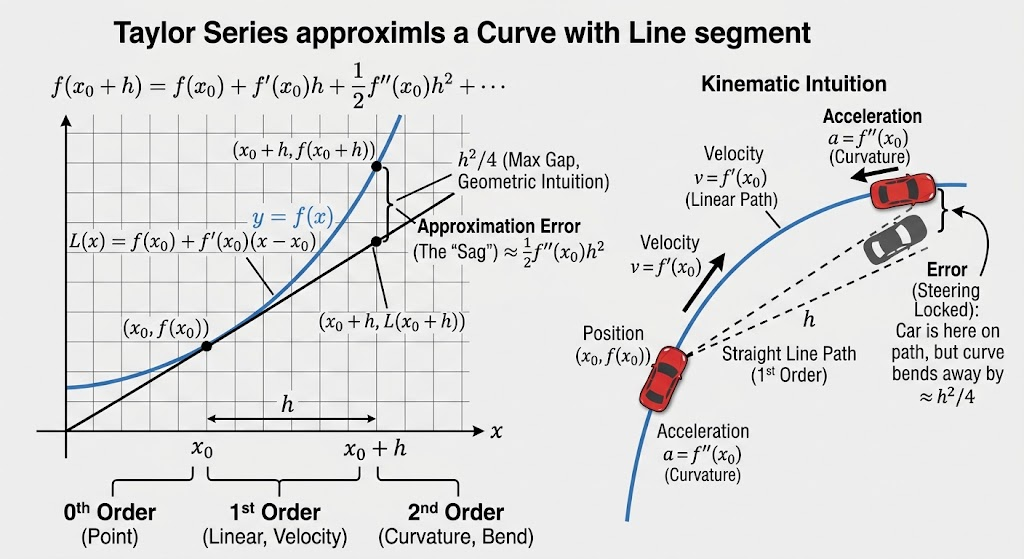
\includegraphics[width=\textwidth]{figs/taylor-tangent-sag.png}
\end{minipage}
}
\end{frame}

\begin{frame}{Aliasing of a wave that vanishes at every station}
\begin{columns}
\column{0.7\textwidth}
\begin{tikzpicture}
\begin{axis}[rep, height=6.4cm, xmin=0, xmax=1, ymin=-1.5, ymax=1.6, xlabel=$x$, ylabel=$u(x)$, legend pos=south west]
\addplot[ink, line width=1.4pt] table[x=x, y=u]{data/string.dat};
\addlegendentry{original}
\addplot[only marks, mark=*, mark size=2pt, sred] table[x=x, y=u]{data/readings17.dat};
\addlegendentry{seventeen readings}
\stepfrom{2}{\addplot[sblue, line width=1.4pt] table[x=x, y=a]{data/alias.dat};
          \addlegendentry{original $+\,0.3\sin(16\pi x)$}}
\end{axis}
\end{tikzpicture}
\column{0.3\textwidth}
\stepfrom{2}{\chip{change in the seventeen readings}{$0$}\\[4pt]
\chip{change at each crest}{$0.3$, about a quarter of the largest displacement}}
\vfill
\live{readings-at-fixed-stations}
\end{columns}
\note{
The seventeen stations are $x_i = i/16$.
Adding $0.3\sin(16\pi x)$ changes the displacement between them.
At every station the added wave is zero, so every reading remains unchanged.

The two displacements are aliases on this grid.
Their difference reaches magnitude $0.3$ between stations, although their sampled values agree.
A reconstruction needs assumptions about the displacement between measurements.
Can coefficients on known shapes describe the curve without fixing measurement locations?
}
\end{frame}

\begin{frame}{Grid dependence of sampled representations}
\begin{columns}
\column{0.7\textwidth}
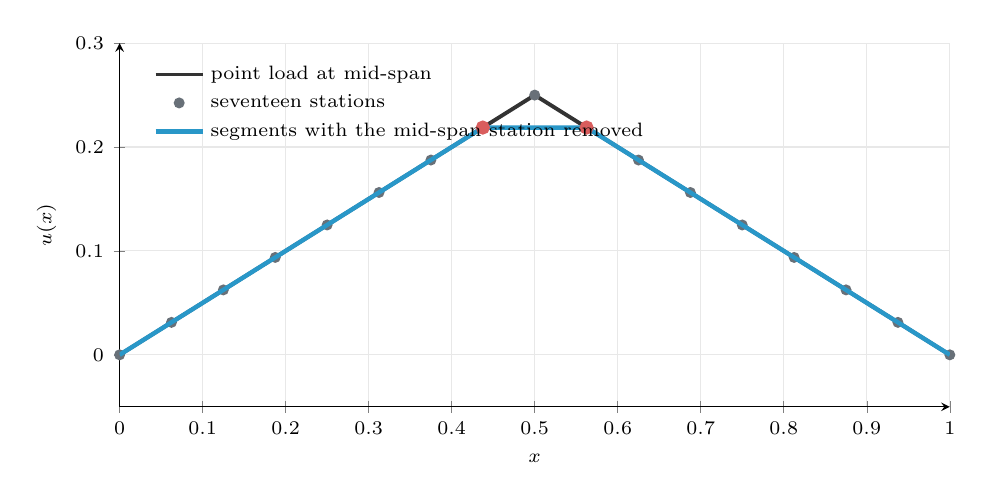
\begin{tikzpicture}
\begin{axis}[rep, height=6.2cm, xmin=0, xmax=1, ymin=-0.05, ymax=0.3, xlabel=$x$, ylabel=$u(x)$, legend pos=north west]
\addplot[ink, line width=1.4pt, domain=0:1, samples=201] {0.5*min(x, 1-x)};
\addlegendentry{point load at mid-span}
\addplot[only marks, mark=*, mark size=1.4pt, muted] coordinates {(0,0) (0.0625,0.03125) (0.125,0.0625) (0.1875,0.09375) (0.25,0.125) (0.3125,0.15625) (0.375,0.1875) (0.4375,0.21875) (0.5,0.25) (0.5625,0.21875) (0.625,0.1875) (0.6875,0.15625) (0.75,0.125) (0.8125,0.09375) (0.875,0.0625) (0.9375,0.03125) (1,0)};
\addlegendentry{seventeen stations}
\stepfrom{2}{\addplot[sblue, line width=1.6pt] coordinates {(0,0) (0.4375,0.21875) (0.5625,0.21875) (1,0)};
          \addlegendentry{segments with the mid-span station removed}
          \addplot[only marks, mark=*, sred] coordinates {(0.4375,0.21875) (0.5625,0.21875)};}
\end{axis}
\end{tikzpicture}
\column{0.3\textwidth}
\stepfrom{2}{\chip{corner, mid-span sensor removed}{worst miss $0$ to $12.5$ percent}\\[4pt]
\chip{smooth displacement, same sensor removed}{$1.6$ to $1.7$ percent}}
\end{columns}
\note{
A sampled representation needs the measurement locations as well as the values.
Lists from different grids cannot be compared entry by entry.
If a sensor fails, the interpolation rule must reconstruct a larger interval.

A point load at mid-span produces two straight segments with a corner.
Seventeen equally spaced stations reproduce this displacement without error because one station lies at the corner.
Removing that station replaces the peak by a horizontal segment at height $0.21875$.
The relative sup error increases from zero to $12.5$ percent.
Removing the same station from the smooth test displacement changes this error from $1.6$ to $1.7$ percent.
How can stored numbers describe shapes rather than values at particular locations?
}
\end{frame}

%========================================================================================
\repsection{Vectors}{Functions as vectors}

\begin{frame}{Representing a function with coefficients on sine modes}
\begin{columns}
\column{0.7\textwidth}
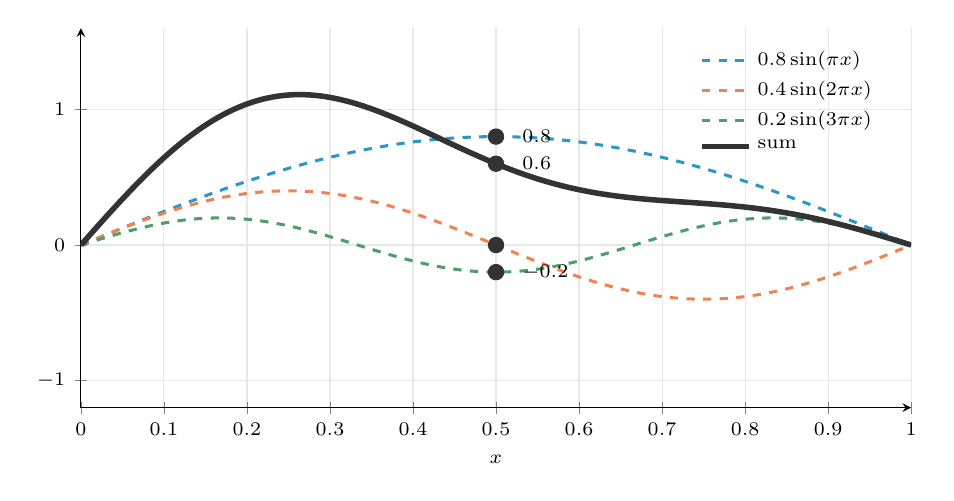
\begin{tikzpicture}
\begin{axis}[rep, height=6.4cm, xmin=0, xmax=1, ymin=-1.2, ymax=1.6, xlabel=$x$, legend pos=north east]
\addplot[sblue, dashed, domain=0:1, samples=201] {0.8*sin(deg(pi*x))};
\addlegendentry{$0.8\sin(\pi x)$}
\stepfrom{2}{\addplot[sorange, dashed, domain=0:1, samples=201] {0.4*sin(deg(2*pi*x))};
          \addlegendentry{$0.4\sin(2\pi x)$}}
\stepfrom{3}{\addplot[sgreen, dashed, domain=0:1, samples=201] {0.2*sin(deg(3*pi*x))};
          \addlegendentry{$0.2\sin(3\pi x)$}}
\stepfrom{4}{\addplot[ink, line width=2pt, domain=0:1, samples=201] {0.8*sin(deg(pi*x)) + 0.4*sin(deg(2*pi*x)) + 0.2*sin(deg(3*pi*x))};
          \addlegendentry{sum}}
\stepfrom{5}{\addplot[only marks, mark=*, mark size=2.4pt, ink] coordinates {(0.5,0.8) (0.5,0) (0.5,-0.2) (0.5,0.6)};
          \node[font=\scriptsize, anchor=west] at (axis cs:0.52,0.8) {$0.8$};
          \node[font=\scriptsize, anchor=west] at (axis cs:0.52,-0.2) {$-0.2$};
          \node[font=\scriptsize, anchor=west] at (axis cs:0.52,0.6) {$0.6$};}
\end{axis}
\end{tikzpicture}
\column{0.3\textwidth}
\stepfrom{4}{\chip{the whole curve}{three numbers, $(0.8, 0.4, 0.2)$}\\[4pt]}
\stepfrom{5}{\chip{check at mid-span}{$u(\tfrac12) = 0.8 - 0.2 = 0.6$}}
\vfill
\live{coefficients-on-shapes}
\end{columns}
\note{
The test displacement is a weighted sum of sine modes.
The first contribution is $0.8\sin(\pi x)$.
Adding $0.4\sin(2\pi x)$ and $0.2\sin(3\pi x)$ reproduces the displacement at every $x$.

The coefficients $(0.8,0.4,0.2)$ describe the curve without a sampling grid.
At mid-span the second mode vanishes, while the first and third have values $1$ and $-1$.
Thus $u(\tfrac12) = 0.8 - 0.2 = 0.6$.
Every mode vanishes at both endpoints, so every such sum satisfies the pinned boundary conditions.
}
\end{frame}

\begin{frame}{A three-parameter family of string displacements}
\begin{center}
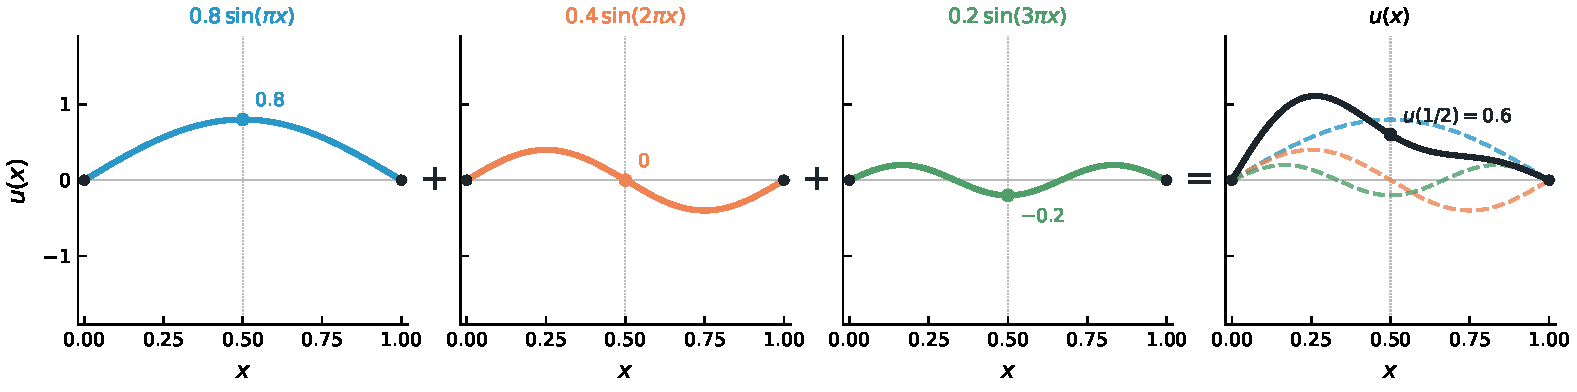
\includegraphics[width=0.64\textwidth]{figs/rep-hero-a}

\stepfrom{2}{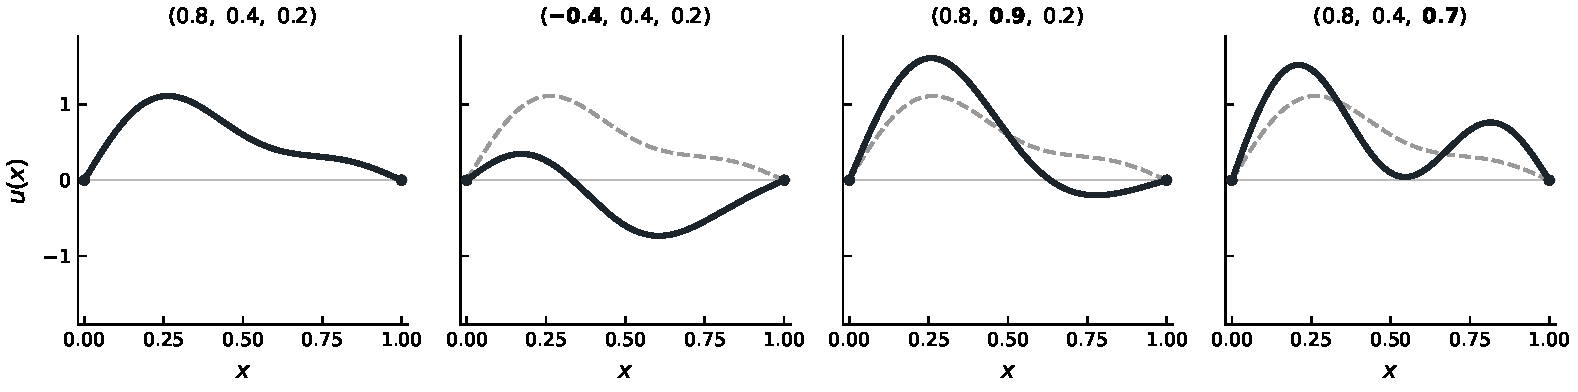
\includegraphics[width=0.64\textwidth]{figs/rep-hero-b}}
\end{center}
\centering
\chip{the family}{$u = a_1\sin(\pi x) + a_2\sin(2\pi x) + a_3\sin(3\pi x)$}\quad
\stepfrom{2}{\chip{one coefficient changes per panel}{$(-0.4, 0.4, 0.2)$, $(0.8, 0.9, 0.2)$, $(0.8, 0.4, 0.7)$}}
\note{
The top row shows each weighted mode and their pointwise sum.
At mid-span their contributions are $0.8$, $0$, and $-0.2$.
Their sum is the displacement value $0.6$.

The bottom row changes one coefficient at a time.
Each change adds a multiple of the corresponding mode to the original displacement.
Because the modes extend across the interval, a coefficient change affects the curve across the interval.
These coefficients give coordinates for the family of three-sine displacements.
}
\end{frame}

\begin{frame}{Matching the displacement with three weights}
\begin{columns}
\column{0.7\textwidth}
\begin{tikzpicture}
\begin{axis}[rep, height=6.4cm, xmin=0, xmax=1, ymin=-0.4, ymax=1.4, xlabel=$x$, ylabel=$u(x)$, legend pos=north east]
\addplot[ink, line width=2pt] table[x=x, y=u]{data/string.dat};
\addlegendentry{displacement, fixed}
\steponly{1}{3}{\addplot[muted, dashed, line width=1.8pt, domain=0:1, samples=201] {0.5*sin(deg(pi*x))};
                \addlegendentry{weights $(0.5, 0, 0)$}}
\steponly{2}{3}{\addplot[muted, dashed, line width=1.8pt, domain=0:1, samples=201] {0.8*sin(deg(pi*x)) + 0.4*sin(deg(2*pi*x))};
                \addlegendentry{weights $(0.8, 0.4, 0)$}}
\steponly{3}{3}{\addplot[muted, dashed, line width=1.8pt, domain=0:1, samples=201] {0.8*sin(deg(pi*x)) + 0.4*sin(deg(2*pi*x)) + 0.2*sin(deg(3*pi*x))};
                \addlegendentry{weights $(0.8, 0.4, 0.2)$}}
\end{axis}
\end{tikzpicture}
\column{0.3\textwidth}
\steponly{1}{3}{\chip{relative sup, $L^2$, slope errors}{$68.5$, $58.8$, $81.5$ percent}\\[4pt]\chip{$L^2$ distance}{$0.381$}}
\steponly{2}{3}{\chip{relative sup, $L^2$, slope errors}{$18.0$, $21.8$, $46.9$ percent}\\[4pt]\chip{$L^2$ distance}{$0.141$}}
\steponly{3}{3}{\chip{relative sup, $L^2$, slope errors}{$0$, $0$, $0$}\\[4pt]\chip{solve, $a_k = 2\int_0^1 u \sin(k\pi x)\,dx$}{$(0.800, 0.400, 0.200)$}}
\vfill
\live{coefficients-on-shapes}
\end{columns}
\note{
Now keep the displacement fixed and start with coefficients $(0.5,0,0)$.
This approximation has relative sup error $68.5$ percent and $L^2$ error $0.381$.
Setting the first two coefficients to $0.8$ and $0.4$ reduces the relative sup error to $18.0$ percent.
The relative slope error remains $46.9$ percent because the third mode is missing.

Setting the third coefficient to $0.2$ makes the error zero in every norm.
The coefficient can also be recovered by integration.
Products of distinct sine modes integrate to zero, while each squared mode integrates to $\tfrac12$.
Consequently $a_k = 2\int_0^1 u(x)\sin(k\pi x)\,dx$ recovers $(0.800,0.400,0.200)$.
}
\end{frame}

\begin{frame}{The coefficient list as coordinates in a vector space}
\begin{columns}
\column{0.5\textwidth}
\begin{figure}
\centering
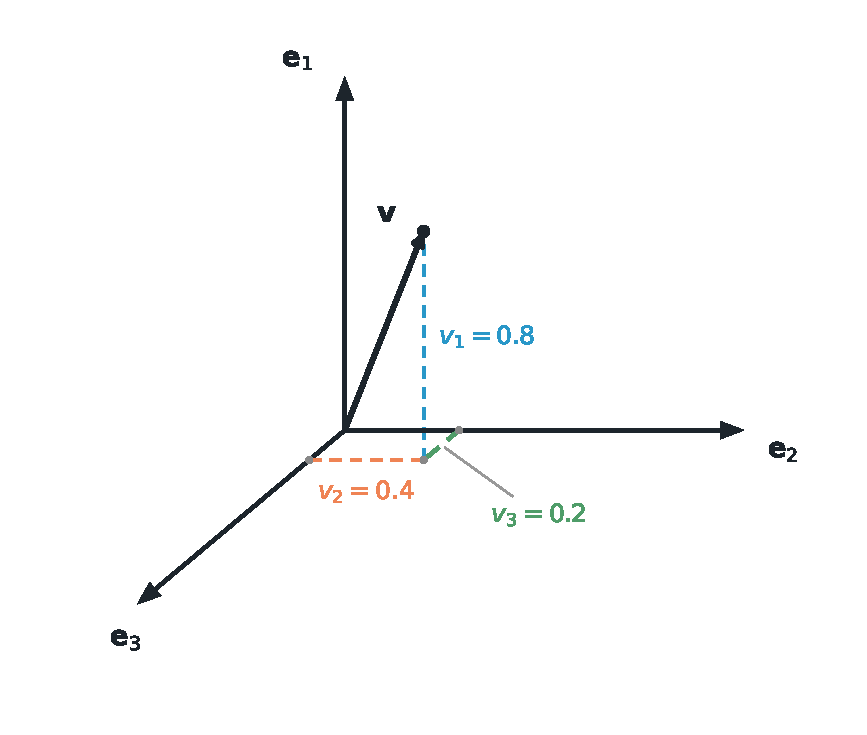
\includegraphics[width=0.7\textwidth]{figs/rep-coordinates-a}
\end{figure}
\column{0.5\textwidth}
\begin{figure}
\centering
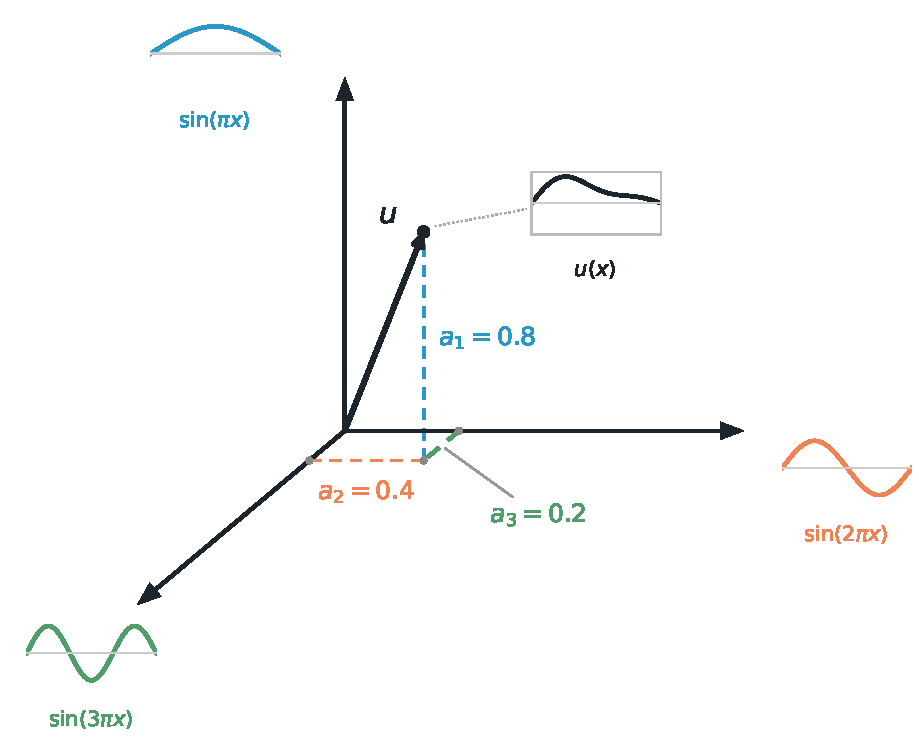
\includegraphics[width=0.7\textwidth]{figs/rep-coordinates-b}
\end{figure}
\end{columns}
\[
u + v = \sum_{i=1}^{3} (a_i + b_i)\,\phi_i, \qquad \alpha u = \sum_{i=1}^{3} (\alpha a_i)\,\phi_i
\]
\note{
The list $(0.8,0.4,0.2)$ specifies a vector in $\mathbb{R}^3$.
The same list specifies a function when its entries weight the three sine modes.
Adding two such functions adds their coefficients, and scaling a function scales its coefficients.
These operations keep the result in the same family.

This family is therefore a linear subspace of the functions on the interval.
The sine modes are linearly independent, so they form a basis of this subspace.
Each function has a unique coefficient list, and the subspace has dimension three.
}
\end{frame}

\begin{frame}{Recovering the coefficients from three readings}
\begin{columns}
\column{0.52\textwidth}
\begin{tikzpicture}
\begin{axis}[rep, height=5.6cm, xmin=0, xmax=1, ymin=-0.2, ymax=1.35, xlabel=$x$, ylabel=$u(x)$]
\addplot[ink, line width=1.6pt] table[x=x, y=u]{data/string.dat};
\addplot[only marks, mark=*, mark size=2.8pt, sred] coordinates {(0.5,0.6)};
\stepfrom{2}{\addplot[only marks, mark=*, mark size=2.8pt, sred] coordinates {(0.25,1.1071) (0.75,0.3071)};}
\end{axis}
\end{tikzpicture}
\column{0.48\textwidth}
\small
\[
\begin{pmatrix} y_1 \\ y_2 \\ y_3 \end{pmatrix}
=
\begin{pmatrix}
1/\sqrt{2} & 1 & 1/\sqrt{2} \\
1 & 0 & -1 \\
1/\sqrt{2} & -1 & 1/\sqrt{2}
\end{pmatrix}
\begin{pmatrix} a_1 \\ a_2 \\ a_3 \end{pmatrix}
\]
\chip{mid-span alone, $y_2 = u(\tfrac12)$}{$a_1 - a_3 = 0.6$, nothing about $a_2$}\\[4pt]
\stepfrom{2}{\chip{quarter spans, $y_1, y_3$}{$1.107$ and $0.307$}\\[4pt]}
\stepfrom{3}{\chip{solved}{$a_2 = \tfrac{y_1 - y_3}{2} = 0.4$, $a_1 + a_3 = \tfrac{y_1 + y_3}{\sqrt2} = 1$, so $(0.8, 0.4, 0.2)$}}
\end{columns}
\note{
Recovering coefficients from readings requires independent information about the modes.
The mid-span reading gives $a_1-a_3=0.6$.
It gives no information about $a_2$ because the second mode vanishes there.

The quarter-span readings provide the missing information.
At $x=1/4$ and $x=3/4$, the second mode has values $1$ and $-1$.
The first and third modes both have value $1/\sqrt2$ at these locations.
The measured displacements are $1.107$ and $0.307$.

Subtracting the quarter-span equations gives $a_2=(y_1-y_3)/2=0.4$.
Adding them gives $a_1+a_3=(y_1+y_3)/\sqrt2=1$.
Together with $a_1-a_3=0.6$, these equations recover $(0.8,0.4,0.2)$.
The measurement matrix has independent, orthogonal columns and condition number one.
Endpoint readings add no information because all the modes vanish there.
}
\end{frame}

\begin{frame}{Approximating a function outside the span}
\begin{columns}
\column{0.7\textwidth}
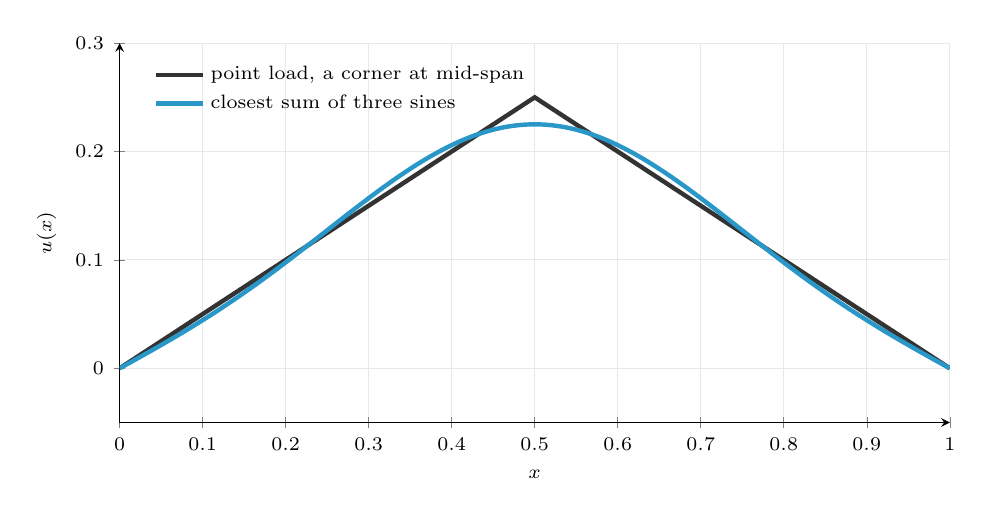
\begin{tikzpicture}
\begin{axis}[rep, height=6.4cm, xmin=0, xmax=1, ymin=-0.05, ymax=0.3, xlabel=$x$, ylabel=$u(x)$, legend pos=north west]
\addplot[ink, line width=1.6pt, domain=0:1, samples=201] {0.5*min(x, 1-x)};
\addlegendentry{point load, a corner at mid-span}
\stepfrom{2}{\addplot[sblue, line width=1.6pt, domain=0:1, samples=301] {0.2026*sin(deg(pi*x)) - 0.0225*sin(deg(3*pi*x))};
          \addlegendentry{closest sum of three sines}}
\end{axis}
\end{tikzpicture}
\column{0.3\textwidth}
\stepfrom{2}{\chip{closest three sines, relative $L^2$ error}{$4.8$ percent}}
\end{columns}
\note{
So far the displacement lies in the span of three smooth sine modes.
A point load produces a displacement with a corner at mid-span.
No finite sum of these smooth modes can reproduce that corner.

The closest three-sine approximation has relative $L^2$ error $4.8$ percent.
A finite-dimensional representation is exact for its own members, but it approximates a general displacement outside that family.
The word closest requires a measure of the error.
Which measure matches the physical question?
}
\end{frame}

%========================================================================================
\repsection{Norms}{Norms and the meaning of error}

\begin{frame}{Measuring value and slope errors}
\begin{columns}[T]
\column{0.33\textwidth}
\begin{tikzpicture}
\begin{axis}[rep, height=5cm, xmin=0, xmax=1, ymin=-0.3, ymax=0.3, xlabel=$x$, title={\scriptsize error $e = u - v$}]
\addplot[name path=E, ink, line width=1.2pt] table[x=x, y=e]{data/error5.dat};
\addplot[name path=Z, draw=none] {0};
\addplot[sgreen!45] fill between[of=E and Z, split, every segment no 1/.style={fill=sred!45}, every segment no 3/.style={fill=sred!45}, every segment no 5/.style={fill=sred!45}];
\addplot[only marks, mark=*, sred, mark size=2.4pt] coordinates {(0.125,0.223)};
\end{axis}
\end{tikzpicture}
\chip{largest gap, sup norm}{$0.22$}
\column{0.33\textwidth}
\begin{tikzpicture}
\begin{axis}[rep, height=5cm, xmin=0, xmax=1, ymin=0, ymax=0.06, xlabel=$x$, title={\scriptsize squared error $e^2$}]
\stepfrom{2}{\addplot[name path=E2, ink, line width=1.2pt] table[x=x, y=e2]{data/error5.dat};
\addplot[name path=Z2, draw=none] {0};
\addplot[syellow!70] fill between[of=E2 and Z2];}
\end{axis}
\end{tikzpicture}
\chip{root of the area, $L^2$ norm}{$0.093$}
\column{0.33\textwidth}
\begin{tikzpicture}
\begin{axis}[rep, height=5cm, xmin=0, xmax=1, ymin=-3.2, ymax=3.2, xlabel=$x$, title={\scriptsize slope error $e'$}]
\stepfrom{3}{\addplot[sorange, line width=1.2pt] table[x=x, y=de]{data/error5.dat};}
\end{axis}
\end{tikzpicture}
\chip{root-mean-square slope, $H^1$ seminorm}{$1.20$}
\end{columns}
\vfill
\hfill\live{coefficients-on-shapes}
\note{
The five-sensor interpolation error is $e=u-v$.
For a clearance calculation, the largest pointwise gap matters.
This gap is the sup norm $\|e\|_\infty=0.22$.

The $L^2$ norm measures the squared error integrated over the interval.
Squaring prevents positive and negative errors from canceling.
Taking the square root gives $\|e\|_{L^2}=0.093$, or $14$ percent of the displacement's $L^2$ norm.

The string's elastic energy depends on its slope.
The slope error has seminorm $|e|_{H^1}=\|e'\|_{L^2}=1.20$, or $42$ percent of the displacement's slope seminorm.
The elastic energy of the error is $\tfrac12|e|_{H^1}^2=0.72$.
An approximation can therefore have a small displacement error and a much larger relative slope error.
}
\end{frame}

\begin{frame}{The $L^2$ distance}
\begin{columns}
\column{0.64\textwidth}
\begin{tikzpicture}
\begin{axis}[rep, height=5.8cm, xmin=0, xmax=1, ymin=-0.4, ymax=1.35, xlabel=$x$, legend pos=north east]
\addplot[sblue, line width=1.6pt] table[x=x, y=u]{data/slid_copy.dat};
\addlegendentry{$u(x)$}
\addplot[sorange, line width=1.6pt] table[x=x, y=g]{data/slid_copy.dat};
\addlegendentry{$u(x - 0.08) + 0.15\sin(6\pi x)$}
\stepfrom{2}{\addplot[name path=U, draw=none, forget plot] table[x=x, y=u]{data/slid_copy.dat};
          \addplot[name path=G, draw=none, forget plot] table[x=x, y=g]{data/slid_copy.dat};
          \addplot[syellow!55, forget plot] fill between[of=U and G];}
\end{axis}
\end{tikzpicture}
\column{0.36\textwidth}
\small
\[
\|u - g\|_{L^2} = \Bigl(\int_0^1 (u - g)^2\,dx\Bigr)^{1/2}
\]
\stepfrom{2}{\chip{$L^2$ distance}{$0.246$}\\[4pt]
\chip{signed integral of the gap}{$0.0275$}}
\vfill
\href{https://sciml-book.github.io/sciml_notebook/representations/norms.html}{\scriptsize\textcolor{burntorange}{\underline{norms notebook}}}
\end{columns}
\note{
The second curve is the displacement shifted $0.08$ to the right, with a small sixth mode added.
The signed integral of their difference is $0.0275$.
This integral does not measure distance because positive and negative differences cancel.

The $L^2$ distance instead squares each difference, integrates, and takes the square root.
For these curves it is $0.246$.
The shaded area represents the squared differences before integration.
The norms notebook varies the shift and the quadrature resolution to approximate the same integral.
}
\end{frame}

\begin{frame}{The sup norm, $L^2$ norm, and slope seminorm can disagree}
\begin{columns}[T]
\column{0.6\textwidth}
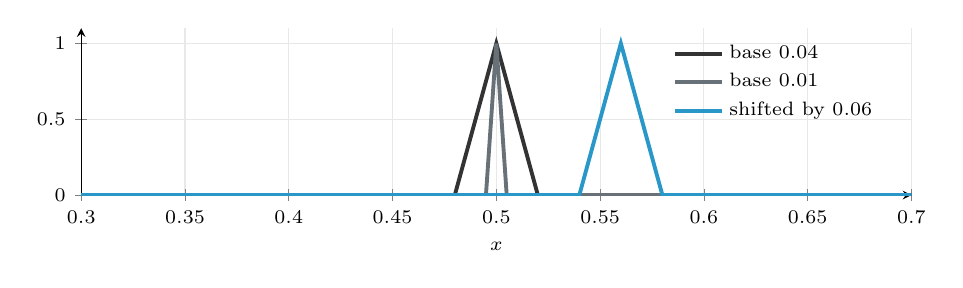
\begin{tikzpicture}
\begin{axis}[rep, height=3.7cm, xmin=0.3, xmax=0.7, ymin=0, ymax=1.1, xlabel=$x$, legend pos=north east]
\addplot[ink, line width=1.4pt, domain=0.3:0.7, samples=401] {max(0, 1 - abs(x-0.5)/0.02)};
\addlegendentry{base $0.04$}
\stepfrom{2}{\addplot[muted, line width=1.4pt, domain=0.3:0.7, samples=801] {max(0, 1 - abs(x-0.5)/0.005)};
          \addlegendentry{base $0.01$}}
\stepfrom{3}{\addplot[sblue, line width=1.4pt, domain=0.3:0.7, samples=401] {max(0, 1 - abs(x-0.56)/0.02)};
          \addlegendentry{shifted by $0.06$}}
\end{axis}
\end{tikzpicture}

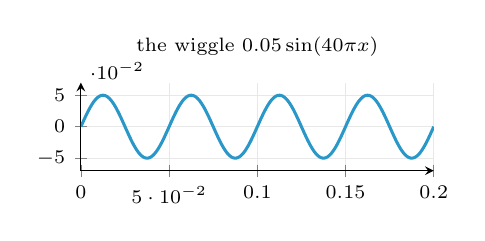
\begin{tikzpicture}
\begin{axis}[rep, width=0.5\linewidth, height=2.7cm, xmin=0, xmax=0.2, ymin=-0.07, ymax=0.07, title={\scriptsize the wiggle $0.05\sin(40\pi x)$}, ytick={-0.05,0,0.05}]
\stepfrom{3}{\addplot[sblue, line width=1.1pt, domain=0:0.2, samples=401] {0.05*sin(deg(40*pi*x))};}
\end{axis}
\end{tikzpicture}%
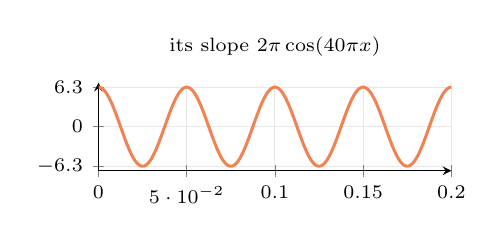
\begin{tikzpicture}
\begin{axis}[rep, width=0.5\linewidth, height=2.7cm, xmin=0, xmax=0.2, ymin=-7, ymax=7, title={\scriptsize its slope $2\pi\cos(40\pi x)$}, ytick={-6.28,0,6.28}, yticklabels={$-6.3$,$0$,$6.3$}]
\stepfrom{3}{\addplot[sorange, line width=1.1pt, domain=0:0.2, samples=401] {2*pi*cos(deg(40*pi*x))};}
\end{axis}
\end{tikzpicture}
\column{0.4\textwidth}
\chip{spike, base $0.04$}{sup $1$, $L^2$ $0.115$, energy $50$}\\[4pt]
\stepfrom{2}{\chip{spike, base $0.01$}{sup $1$, $L^2$ $0.058$, energy $200$}\\[4pt]}
\stepfrom{3}{\chip{$L^2$ distance, spike to shifted spike}{$\sqrt2 \times 0.115 = 0.163$}\\[4pt]
\chip{wiggle $0.05\sin(40\pi x)$}{sup $0.05$, $L^2$ $0.035$, slope seminorm $4.44$}}
\vfill
\live{coefficients-on-shapes}
\end{columns}
\note{
Consider a triangular spike of height one and base width $b=0.04$.
Its sup norm is one, its $L^2$ norm is $\sqrt{b/3}=0.115$, and its elastic energy is $2/b=50$.
Quartering the width leaves the sup norm unchanged, halves the $L^2$ norm to $0.058$, and increases the energy to $200$.
Thus no uniform constant bounds the sup norm by the $L^2$ norm over this family.

Moving the spike until its support is disjoint from the original gives $L^2$ distance $\sqrt2\times0.115=0.163$.
The squared distance is the sum of the two squared norms because the product of the spikes is zero.
As the width tends to zero, the spike's energy diverges even though its $L^2$ norm tends to zero.

High frequency also increases the slope error.
The wave $0.05\sin(40\pi x)$ has sup norm $0.05$ and $L^2$ norm $0.035$.
Its slope has amplitude $6.3$ and $H^1$ seminorm $4.44$.
These measures distinguish displacement amplitude from variation in space.
}
\end{frame}

\begin{frame}{Definition of a norm and a seminorm}
\begin{block}{Norm}
For functions $u,v$ in a real vector space and a scalar $\alpha$, a norm satisfies
\[
\begin{aligned}
&\|u\|\ge0,\qquad \|u\|=0 \iff u=0,\\
&\|\alpha u\|=|\alpha|\,\|u\|,\qquad \|u+v\|\le\|u\|+\|v\|.
\end{aligned}
\]
\end{block}
\medskip
\begin{block}{Seminorm}
The slope seminorm vanishes on every constant function.
\[
|c|_{H^1}=\|c'\|_{L^2}=0.
\]
Pinning excludes nonzero constants, so this seminorm is a norm on pinned finite-energy displacements.
\end{block}
\note{
Adding a constant to a displacement leaves its slope unchanged.
The slope quantity $\|u'\|_{L^2}$ therefore assigns zero to every constant function.
On a space containing nonzero constants, this quantity is a seminorm.

A norm assigns a nonnegative number to each function.
Only the zero function has norm zero.
Scaling a function by $\alpha$ multiplies its norm by $|\alpha|$, and the norm of a sum is at most the sum of the norms.
The sup and $L^2$ measures satisfy these properties on their respective function spaces.

For pinned displacements, zero slope implies a constant displacement, and the endpoint conditions force that constant to be zero.
The slope seminorm is therefore a norm on the pinned finite-energy space.
Each norm defines a distance by measuring the difference, $\|u-v\|$.
The closest approximation depends on which of these distances is minimized.
}
\end{frame}

\begin{frame}{Closest three-sine sums to the corner in the $L^2$ and sup norms}
\begin{columns}[T]
\column{0.5\textwidth}
\begin{tikzpicture}
\begin{axis}[rep, height=4.6cm, xmin=0, xmax=1, ymin=-0.02, ymax=0.29, xlabel=$x$, title={\scriptsize the corner (black), closest in $L^2$ (blue) and in sup (orange)}]
\addplot[ink, line width=1.6pt] table[x=x, y=u]{data/corner_sums.dat};
\addplot[sblue, dashed, line width=1.4pt] table[x=x, y=vl2]{data/corner_sums.dat};
\stepfrom{2}{\addplot[sorange, dashed, line width=1.4pt] table[x=x, y=vsup]{data/corner_sums.dat};}
\end{axis}
\end{tikzpicture}
\column{0.5\textwidth}
\begin{tikzpicture}
\begin{axis}[rep, height=4.6cm, xmin=0, xmax=1, ymin=-0.03, ymax=0.03, xlabel=$x$, title={\scriptsize the gap $u - v$}, scaled y ticks=false, yticklabel style={/pgf/number format/fixed}]
\addplot[sblue, line width=1.3pt] table[x=x, y=el2]{data/corner_sums.dat};
\stepfrom{2}{\addplot[sorange, line width=1.3pt] table[x=x, y=esup]{data/corner_sums.dat};}
\end{axis}
\end{tikzpicture}
\end{columns}
\smallskip
\centering
\chip{$L^2$-closest, $(0.2026, 0, -0.0225)$}{sup $9.9$, $L^2$ $4.8$, slope $31.5$ percent}\quad
\stepfrom{2}{\chip{sup-closest, $(0.2045, 0, -0.0318)$}{sup $5.5$, $L^2$ $6.7$, slope $33.9$ percent}}
\note{
The corner has different closest three-sine approximations in the $L^2$ and sup norms.
Its $L^2$ projection has coefficients $c_k=2\sin(k\pi/2)/(k\pi)^2$, giving $(0.2026,0,-0.0225)$.
Its relative errors are $9.9$ percent in sup, $4.8$ percent in $L^2$, and $31.5$ percent in the slope seminorm.

Minimizing the largest gap gives coefficients $(0.2045,0,-0.0318)$.
The relative errors become $5.5$ percent in sup, $6.7$ percent in $L^2$, and $33.9$ percent in the slope seminorm.
Reducing the largest gap increases the errors measured by the other norms.

The $L^2$ and energy projections coincide for these Dirichlet sine modes.
Integration by parts multiplies both the projection numerator and denominator by $(k\pi)^2$, leaving each coefficient unchanged.
Orthogonality in both inner products alone would not establish this equality.
How does orthogonality determine the projection coefficients?
}
\end{frame}

%========================================================================================
\repsection{Spaces}{Function spaces, $L^2$, $H^1$, and Hilbert spaces}

\begin{frame}{The space $L^2$ of square-integrable functions}
\begin{columns}
\column{0.58\textwidth}
\begin{tikzpicture}
\begin{axis}[rep, height=5.6cm, xmin=0, xmax=1, ymin=0, ymax=6.2, xlabel=$x$, legend pos=north east]
\addplot[sblue, line width=1.6pt] table[x=x, y=step]{data/l2_members.dat};
\addlegendentry{step, in $L^2$}
\stepfrom{2}{\addplot[sgreen, line width=1.6pt] table[x=x, y=cube]{data/l2_members.dat};
          \addlegendentry{$x^{-1/3}$, in $L^2$}}
\stepfrom{3}{\addplot[sred, dashed, line width=1.6pt] table[x=x, y=half]{data/l2_members.dat};
          \addlegendentry{$x^{-1/2}$, not in $L^2$}}
\end{axis}
\end{tikzpicture}
\column{0.42\textwidth}
\small
\[
\|f\|_{L^2}^2 = \int_0^1 f(x)^2\,dx < \infty
\]
\[
\langle f, g\rangle = \int_0^1 f g\,dx
\]
\stepfrom{2}{\chip{$\int_0^1 (x^{-1/3})^2\,dx$}{$3$, finite although $x^{-1/3}$ is unbounded}\\[4pt]}
\stepfrom{3}{\chip{$\int_0^1 (x^{-1/2})^2\,dx = \int_0^1 x^{-1}\,dx$}{diverges}\\[4pt]}
\chip{two functions equal except at one point}{$L^2$ distance $0$}
\end{columns}
\note{
The step has a finite integral of its square despite its jump.
The function $x^{-1/3}$ also has a finite squared integral, $\int_0^1 x^{-2/3}\,dx=3$, despite being unbounded near zero.
The function $x^{-1/2}$ fails this test because $\int_0^1 1/x\,dx$ diverges.
These examples distinguish square integrability from continuity and boundedness.

The measurable functions with finite squared integral define $L^2(0,1)$.
Functions equal almost everywhere represent the same element of this space.
Changing a value at one point leaves the $L^2$ distance zero, so point evaluation is not well defined on an arbitrary $L^2$ element.
The inner product $\int_0^1 fg\,dx$ is well defined.
What additional condition controls slopes?
}
\end{frame}

\begin{frame}{The space $H^1$ of finite-energy functions}
\begin{columns}[T]
\column{0.5\textwidth}
\begin{tikzpicture}
\begin{axis}[rep, height=3.9cm, xmin=0, xmax=1, ymin=-0.7, ymax=0.7, xlabel=$x$, title={\scriptsize the corner $\min(x, 1-x)/2$ and its slope, in $H^1_0$}]
\addplot[ink, line width=1.6pt] table[x=x, y=u]{data/corner_slope.dat};
\addplot[sorange, line width=1.4pt] table[x=x, y=du]{data/corner_slope.dat};
\end{axis}
\end{tikzpicture}
\column{0.5\textwidth}
\begin{tikzpicture}
\begin{axis}[rep, height=3.9cm, xmin=0, xmax=1, ymin=-0.2, ymax=21, xlabel=$x$, title={\scriptsize ramps toward a step, and their slopes $1/w$}]
\stepfrom{2}{\addplot[sblue!50, line width=1.4pt] table[x=x, y=dr]{data/ramp_w20.dat};
\addplot[sblue, line width=1.4pt] table[x=x, y=dr]{data/ramp_w5.dat};}
\end{axis}
\end{tikzpicture}
\end{columns}
\small
\[
\|u\|_{H^1}^2 = \int_0^1 u^2\,dx + \int_0^1 (u')^2\,dx, \qquad \langle u, v\rangle_{H^1} = \int_0^1 (u v + u' v')\,dx
\]
\centering
\stepfrom{2}{\chip{ramp of width $w$, $\int (u')^2\,dx$}{$1/w$, so $5$ at $w = 0.2$ and $20$ at $w = 0.05$}\quad}
\stepfrom{3}{\chip{in one dimension}{$|u(y) - u(x)| \le \sqrt{|y - x|}\,\|u'\|_{L^2}$}}
\note{
The point-load displacement is continuous and has slopes $\tfrac12$ and $-\tfrac12$ on the two halves of the interval.
Its classical derivative fails at the corner, but the piecewise-constant slope is square integrable.
Integration by parts still gives $\int u\psi'\,dx=-\int u'\psi\,dx$ for every smooth test function $\psi$ supported inside the interval.
A derivative defined by this identity is a weak derivative.

The functions in $L^2$ with a weak derivative in $L^2$ form the Sobolev space $H^1(0,1)$.
Its squared norm is $\|u\|_{H^1}^2=\|u\|_{L^2}^2+\|u'\|_{L^2}^2$.
The point-load displacement belongs to this space, whereas a step does not.
A ramp of width $w$ has squared slope integral $1/w$, which grows without bound as it approaches a step.

On an interval, the slope bound gives $|u(y)-u(x)|\le\sqrt{|y-x|}\,\|u'\|_{L^2}$.
Every $H^1$ element therefore has a unique continuous representative.
This conclusion does not extend to $H^1$ in higher dimensions.
Imposing zero endpoint values gives the pinned space $H^1_0(0,1)$.
}
\end{frame}

\begin{frame}{Equal $L^2$ norm, increasing slope seminorm}
\begin{columns}
\column{0.62\textwidth}
\begin{tikzpicture}
\begin{axis}[rep, height=5.6cm, xmin=0, xmax=1, ymin=-1.6, ymax=1.6, xlabel=$x$, legend style={at={(0.5,1.02)}, anchor=south, legend columns=3}]
\addplot[sblue, line width=1.5pt] table[x=x, y=v]{data/mode1.dat};
\addlegendentry{$k = 1$}
\stepfrom{2}{\addplot[sorange, line width=1.3pt] table[x=x, y=v]{data/mode4.dat};
          \addlegendentry{$k = 4$}}
\stepfrom{3}{\addplot[sgreen, line width=1pt] table[x=x, y=v]{data/mode16.dat};
          \addlegendentry{$k = 16$}}
\end{axis}
\end{tikzpicture}
\column{0.38\textwidth}
\small
\[
\phi_k(x) = \sqrt2\,\sin(k\pi x)
\]
\[
\|\phi_k\|_{L^2} = 1, \qquad |\phi_k|_{H^1} = k\pi
\]
\chip{$|\phi_k|_{H^1}$ at $k = 1$}{$3.14$}\\[4pt]
\stepfrom{2}{\chip{$k = 4$}{$12.57$}\\[4pt]}
\stepfrom{3}{\chip{$k = 16$}{$50.27$}\\[4pt]
\chip{distance between two different modes}{$\sqrt2 = 1.414$}}
\end{columns}
\note{
The normalized modes $\phi_k=\sqrt2\sin(k\pi x)$ all have $L^2$ norm one.
Their slope seminorms are $k\pi$.
For $k=1$, $4$, and $16$, these are $3.14$, $12.57$, and $50.27$.
Increasing frequency leaves the displacement norm unchanged while increasing the slope seminorm.

Distinct modes are orthogonal, so their $L^2$ distance is $\sqrt2$.
The sequence of modes therefore has no $L^2$-convergent subsequence.
A bound on displacement alone does not limit spatial oscillation.
}
\end{frame}

\begin{frame}{Hilbert spaces and the nesting $H^1_0 \subset H^1 \subset L^2$}
\begin{columns}
\column{0.55\textwidth}
\begin{center}
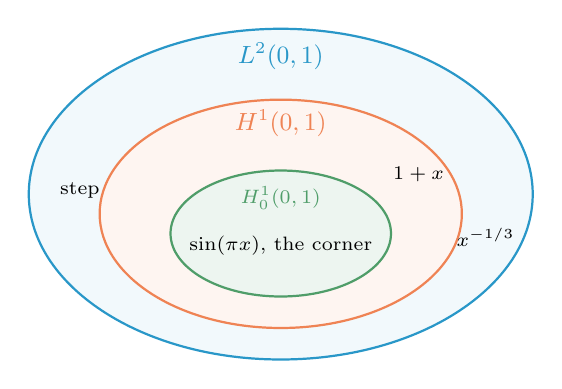
\begin{tikzpicture}[font=\small]
\draw[sblue, thick, fill=sblue!6] (0,0) ellipse (3.2cm and 2.1cm);
\node[sblue] at (0,1.75) {$L^2(0,1)$};
\draw[sorange, thick, fill=sorange!8] (0,-0.25) ellipse (2.3cm and 1.45cm);
\node[sorange] at (0,0.9) {$H^1(0,1)$};
\draw[sgreen, thick, fill=sgreen!10] (0,-0.5) ellipse (1.4cm and 0.8cm);
\node[sgreen, font=\scriptsize] at (0,-0.05) {$H^1_0(0,1)$};
\node[font=\scriptsize, align=center] at (0,-0.65) {$\sin(\pi x)$, the corner};
\node[font=\scriptsize, align=center] at (1.75,0.25) {$1 + x$};
\node[font=\scriptsize, align=center] at (-2.55,0.05) {step};
\node[font=\scriptsize, align=center] at (2.6,-0.55) {$x^{-1/3}$};
\end{tikzpicture}
\end{center}
\column{0.45\textwidth}
\small
\begin{block}{Hilbert space}
A vector space with an inner product in which every Cauchy sequence converges to a member of the space.
\end{block}
\chip{Hilbert spaces}{$\mathbb{R}^n$, $L^2(0,1)$, $H^1(0,1)$, $H^1_0(0,1)$}\\[4pt]
\stepfrom{2}{\chip{not complete}{continuous functions with the $L^2$ distance}}
\end{columns}
\note{
The pinned sine and point-load displacement belong to $H^1_0$.
The line $1+x$ belongs to $H^1$ but fails the zero endpoint conditions.
The step belongs to $L^2$ but lacks a square-integrable weak derivative.
Thus $H^1_0\subset H^1\subset L^2$.

Continuous ramps approaching a step form a Cauchy sequence in the $L^2$ norm.
Their limit lies outside the continuous functions but inside $L^2$.
A space is complete when every Cauchy sequence converges to an element of the space.
A complete inner-product space is a Hilbert space.

The spaces $L^2$, $H^1$, and $H^1_0$ are Hilbert spaces with the indicated inner products.
Projection onto an infinite-dimensional trial space requires that linear subspace to be closed as well.
These conditions guarantee a unique closest element.
Completeness alone does not guarantee a minimizer over an arbitrary family.
}
\end{frame}

\begin{frame}{The space $H^1_0$ and the Poincar\'e inequality}
\begin{columns}
\column{0.48\textwidth}
\begin{tikzpicture}
\begin{axis}[rep, height=4.3cm, xmin=0, xmax=1, ymin=-0.1, ymax=1.2, xlabel=$x$, legend style={at={(0.5,1.02)}, anchor=south, legend columns=3, font=\scriptsize}]
\stepfrom{2}{\addplot[sblue, line width=1.6pt] table[x=x, y=sine]{data/poincare.dat};
\addlegendentry{$\sin(\pi x)$}
\addplot[ink, line width=1.6pt] table[x=x, y=corner]{data/poincare.dat};
\addlegendentry{corner}}
\stepfrom{3}{\addplot[sred, dashed, line width=1.6pt] table[x=x, y=one]{data/poincare.dat};
\addlegendentry{$u = 1$}}
\end{axis}
\end{tikzpicture}
\column{0.52\textwidth}
\small
\[
H^1_0(0,1) = \{\, u \in H^1(0,1) : u(0) = u(1) = 0 \,\}
\]
\[
\|u\|_{L^2} \le \frac{1}{\pi}\,|u|_{H^1} \quad \text{for } u \in H^1_0(0,1)
\]
\stepfrom{3}{\[
|u|_{H^1}^2 \le \|u\|_{H^1}^2 \le \Bigl(1 + \frac{1}{\pi^2}\Bigr)|u|_{H^1}^2 \quad \text{on } H^1_0
\]}
\end{columns}
\vspace{4pt}
\centering
\stepfrom{2}{\chip{$\|u\|_{L^2}/|u|_{H^1}$ for $\sin(\pi x)$}{$0.3183 = 1/\pi$, equality}\quad
\chip{for the corner}{$0.1443/0.5 = 0.2887$}\quad}
\stepfrom{3}{\chip{$u = 1$, in $H^1$ only}{$|u|_{H^1} = 0$, the bound fails}}
\note{
For a pinned displacement, the endpoint values are zero.
On the interval, an $H^1$ element has a unique continuous representative, so these values are well defined.
The endpoint map $\gamma u=(u(0),u(1))$ is called the trace.
Its kernel is $H^1_0(0,1)$.

Pinning controls the displacement norm by the slope seminorm.
Expanding in normalized sine modes gives $\|u\|_{L^2}^2=\sum c_k^2$ and $|u|_{H^1}^2=\sum(k\pi)^2c_k^2$.
Since $k\ge1$, the second sum is at least $\pi^2$ times the first.
This gives the Poincar\'e inequality $\|u\|_{L^2}\le |u|_{H^1}/\pi$.

The lowest mode attains the ratio $1/\pi=0.3183$.
The corner gives $0.2887$ and the three-sine displacement gives $0.2278$.
Without pinning, the constant $u=1$ has zero slope and $L^2$ norm one, so the bound fails.

On $H^1_0$, the inequality gives $|u|_{H^1}^2\le\|u\|_{H^1}^2\le(1+1/\pi^2)|u|_{H^1}^2$.
The slope norm and full $H^1$ norm therefore define the same convergence.
For a bounded Lipschitz domain, the trace and its zero kernel extend to higher dimensions.
The Poincar\'e constant is then $1/\sqrt{\lambda_1}$, where $\lambda_1$ is the lowest Dirichlet eigenvalue.
}
\end{frame}

\begin{frame}{The spaces $L^2$, $H^1$, and $H^1_0$ compared}
\footnotesize
\renewcommand{\arraystretch}{1.6}
\begin{center}
\begin{tabular}{l c c P{3.3cm} P{2.6cm} P{3.4cm}}
\hline
space & $u \in L^2$ & $\nabla u \in L^2$ & inner product & boundary values & role in $-\Delta u = f$ \\
\hline
$L^2(\Omega)$ & \stepfrom{2}{yes} & \stepfrom{2}{not required} & \stepfrom{2}{$\int_\Omega u v\,dx$} & \stepfrom{2}{no general trace or point evaluation} & \stepfrom{2}{square-integrable loads and value misfits} \\
$H^1(\Omega)$ & \stepfrom{2}{yes} & \stepfrom{2}{yes} & \stepfrom{2}{$\int_\Omega (u v + \nabla u\cdot\nabla v)\,dx$} & \stepfrom{2}{trace exists, none imposed} & \stepfrom{2}{free (Neumann) boundaries, imposed through the weak form} \\
$H^1_0(\Omega)$ & \stepfrom{2}{yes} & \stepfrom{2}{yes} & \stepfrom{2}{$\int_\Omega \nabla u\cdot\nabla v\,dx$} & \stepfrom{2}{$u = 0$ on $\partial\Omega$} & \stepfrom{2}{trial and test space for fixed (Dirichlet) boundaries} \\
\hline
\end{tabular}
\end{center}
\note{
The table compares these spaces on a bounded Lipschitz domain $\Omega$.
The square-integrable loads and integrated value errors use $L^2$.
An arbitrary $L^2$ element has no well-defined point evaluation or boundary trace.
The space $H^1$ adds square-integrable weak gradients and a boundary trace.

The space $H^1_0$ imposes zero trace.
It is the trial and test space for the pinned string and a membrane fixed at its boundary.
With flux boundary conditions, the weak formulation instead uses functions whose boundary values are not prescribed.
A purely Neumann Poisson problem also needs a compatibility condition and determines the solution only up to a constant.

The $L^2$ inner product integrates $uv$.
The $H^1$ inner product adds the product of the gradients.
On $H^1_0$, Poincar\'e's inequality makes the gradient term alone an inner product.
On all of $H^1$, nonzero constants prevent that conclusion.
}
\end{frame}

\begin{frame}{Compactness from bounded energy}
\begin{columns}
\column{0.5\textwidth}
\small
\[
u = \sum_{k \ge 1} c_k\,\sqrt2\sin(k\pi x), \qquad |u|_{H^1}^2 = \sum_{k \ge 1} (k\pi)^2 c_k^2
\]
\stepfrom{2}{\[
|u|_{H^1} \le M \;\Longrightarrow\; \Bigl(\sum_{k > K} c_k^2\Bigr)^{1/2} \le \frac{M}{(K+1)\pi}
\]}
\column{0.5\textwidth}
\chip{unit ball of $L^2$}{the modes stay $\sqrt2$ apart, no subsequence converges}\\[4pt]
\stepfrom{2}{\chip{$M = 10$, tail beyond $K = 4$}{at most $0.637$}\\[4pt]
\chip{$M = 10$, tail beyond $K = 16$}{at most $0.187$}\\[4pt]}
\stepfrom{3}{\chip{Rellich, on a bounded interval}{a bounded sequence in $H^1_0$ has an $L^2$-convergent subsequence}}
\end{columns}
\note{
In $\mathbb{R}^n$, every bounded sequence has a convergent subsequence.
The normalized sine modes show why this fails in $L^2$.
They all have norm one, yet distinct modes remain $\sqrt2$ apart.

A bound on the slope seminorm also bounds the high-frequency coefficients.
If $|u|_{H^1}\le M$, then $\sum_{k>K}c_k^2\le M^2/((K+1)\pi)^2$.
Truncation after mode $K$ therefore gives $L^2$ error at most $M/((K+1)\pi)$.
For $M=10$, this bound is $0.637$ after mode $4$ and $0.187$ after mode $16$.

The bound makes the high-frequency remainder uniformly small.
The finitely many remaining coefficients have convergent subsequences.
Together these facts give an $L^2$-convergent subsequence for every bounded sequence in $H^1_0(0,1)$.
This is the compact embedding expressed by Rellich's theorem on the interval.
}
\end{frame}

\begin{frame}{Regularity from the load to the displacement}
\begin{columns}[T]
\column{0.33\textwidth}
\begin{tikzpicture}
\begin{axis}[rep, height=4.6cm, xmin=0, xmax=1, ymin=-0.6, ymax=0.6, xlabel=$x$, title={\scriptsize point load, $u \in H^1_0$}]
\addplot[ink, line width=1.5pt] table[x=x, y=up]{data/reg_loads.dat};
\addplot[sorange, line width=1.2pt] table[x=x, y=dup]{data/reg_loads.dat};
\end{axis}
\end{tikzpicture}
\column{0.33\textwidth}
\begin{tikzpicture}
\begin{axis}[rep, height=4.6cm, xmin=0, xmax=1, ymin=-2.2, ymax=1.2, xlabel=$x$, title={\scriptsize step load, $u \in H^2$}]
\stepfrom{2}{\addplot[ink, line width=1.5pt] table[x=x, y=us]{data/reg_loads.dat};
\addplot[sorange, line width=1.2pt] table[x=x, y=dus]{data/reg_loads.dat};
\addplot[sgreen, line width=1.2pt] table[x=x, y=ddus]{data/reg_loads.dat};}
\end{axis}
\end{tikzpicture}
\column{0.33\textwidth}
\begin{tikzpicture}
\begin{axis}[rep, height=4.6cm, xmin=0, xmax=1, ymin=-2.2, ymax=1.2, xlabel=$x$, title={\scriptsize uniform load, $u = x(1-x)$}]
\stepfrom{3}{\addplot[ink, line width=1.5pt] table[x=x, y=uu]{data/reg_loads.dat};
\addplot[sorange, line width=1.2pt] table[x=x, y=duu]{data/reg_loads.dat};
\addplot[sgreen, line width=1.2pt] table[x=x, y=dduu]{data/reg_loads.dat};}
\end{axis}
\end{tikzpicture}
\end{columns}
\centering
{\scriptsize $u$ black, $u'$ orange, $u''$ green}\\[3pt]
\chip{point load}{slope jumps, $c_k \sim 1/k^2$}\quad
\stepfrom{2}{\chip{step load in $L^2$}{curvature jumps, $u'' \in L^2$}\quad}
\stepfrom{3}{\chip{uniform load}{smooth inside, $c_k \sim 1/k^3$}}
\note{
The load determines the displacement's regularity through $-u''=f$.
A point load is a distribution, and it gives a displacement with a corner.
A square-integrable load gives $u''\in L^2$ and hence $u\in H^2$ on this interval.

The step load gives a continuous slope and a curvature that jumps at mid-span.
The uniform load $f=2$ gives the smooth parabola $x(1-x)$.
The point-load corner belongs to $H^1_0$ but not to $H^2$.

The equation also relates the sine coefficients.
For each mode, it divides the load coefficient by $(k\pi)^2$ to obtain the displacement coefficient.
This produces $1/k^2$ decay for the corner and $1/k^3$ decay for the parabola.
The weak formulation requires only one weak derivative of the displacement, so continuous piecewise-linear hats are admissible.
}
\end{frame}

\repsection{Projection}{Inner products, projection, and orthogonality}

\begin{frame}{The inner product as signed overlap}
\centering\scriptsize $f = \sin(\pi x)$ blue, $g$ orange, and below them $fg$, green where positive and red where negative
\begin{columns}[T]
\column{0.33\textwidth}
\centering
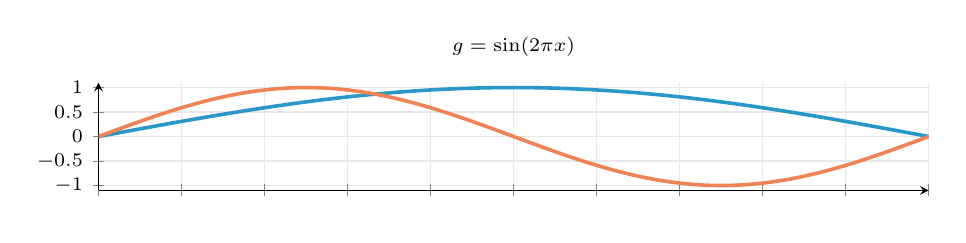
\begin{tikzpicture}
\begin{axis}[rep, width=\linewidth, height=2.95cm, xmin=0, xmax=1, ymin=-1.1, ymax=1.1, title={\scriptsize $g = \sin(2\pi x)$}, xticklabels={}]
\addplot[sblue, line width=1.3pt, domain=0:1, samples=161] {sin(deg(pi*x))};
\addplot[sorange, line width=1.3pt, domain=0:1, samples=161] {sin(deg(2*pi*x))};
\end{axis}
\end{tikzpicture}

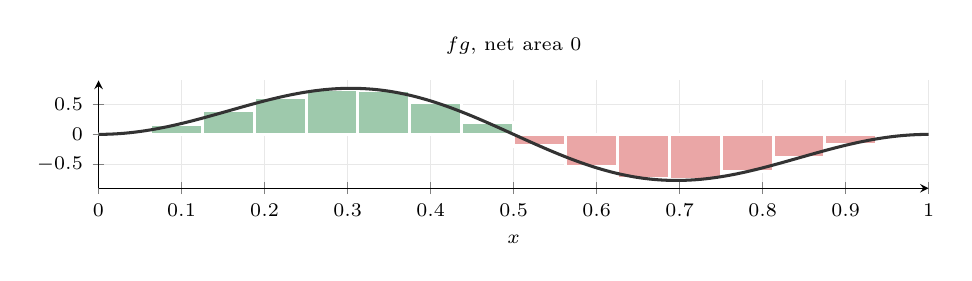
\begin{tikzpicture}
\begin{axis}[rep, width=\linewidth, height=2.95cm, xmin=0, xmax=1, ymin=-0.9, ymax=0.9, xlabel=$x$, title={\scriptsize $fg$, net area $0$}]
\stepfrom{2}{\addplot[ybar, bar width=0.0625, fill=sgreen!55, draw=white, samples at={0.03125,0.09375,0.15625,0.21875,0.28125,0.34375,0.40625,0.46875,0.53125,0.59375,0.65625,0.71875,0.78125,0.84375,0.90625,0.96875}] {max(sin(deg(pi*x))*sin(deg(2*pi*x)),0)};
\addplot[ybar, bar width=0.0625, fill=sred!55, draw=white, samples at={0.03125,0.09375,0.15625,0.21875,0.28125,0.34375,0.40625,0.46875,0.53125,0.59375,0.65625,0.71875,0.78125,0.84375,0.90625,0.96875}] {min(sin(deg(pi*x))*sin(deg(2*pi*x)),0)};
\addplot[ink, line width=1.1pt, domain=0:1, samples=161] {sin(deg(pi*x))*sin(deg(2*pi*x))};}
\end{axis}
\end{tikzpicture}
\column{0.33\textwidth}
\centering
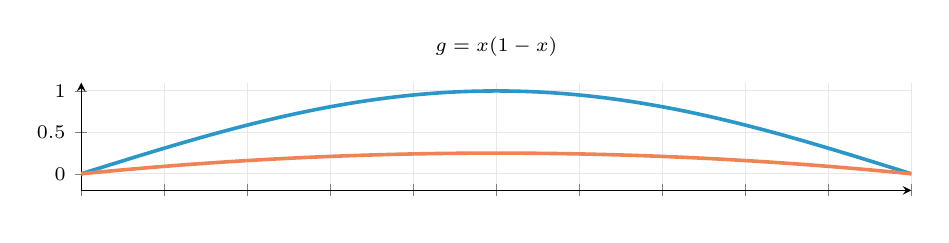
\begin{tikzpicture}
\begin{axis}[rep, width=\linewidth, height=2.95cm, xmin=0, xmax=1, ymin=-0.2, ymax=1.1, title={\scriptsize $g = x(1-x)$}, xticklabels={}]
\addplot[sblue, line width=1.3pt, domain=0:1, samples=161] {sin(deg(pi*x))};
\addplot[sorange, line width=1.3pt, domain=0:1, samples=161] {x*(1-x)};
\end{axis}
\end{tikzpicture}

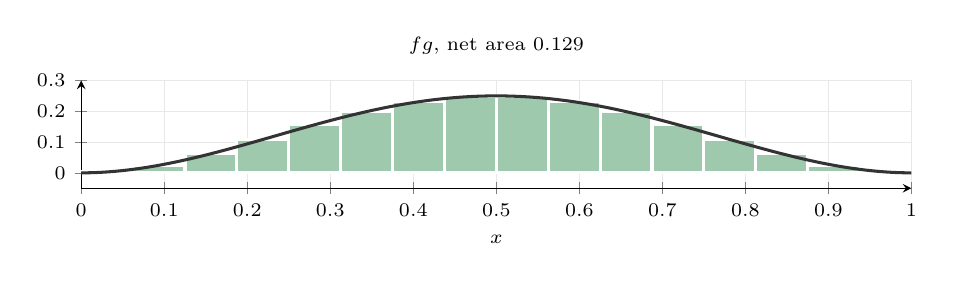
\begin{tikzpicture}
\begin{axis}[rep, width=\linewidth, height=2.95cm, xmin=0, xmax=1, ymin=-0.05, ymax=0.3, xlabel=$x$, title={\scriptsize $fg$, net area $0.129$}]
\stepfrom{2}{\addplot[ybar, bar width=0.0625, fill=sgreen!55, draw=white, samples at={0.03125,0.09375,0.15625,0.21875,0.28125,0.34375,0.40625,0.46875,0.53125,0.59375,0.65625,0.71875,0.78125,0.84375,0.90625,0.96875}] {max(sin(deg(pi*x))*x*(1-x),0)};
\addplot[ybar, bar width=0.0625, fill=sred!55, draw=white, samples at={0.03125,0.09375,0.15625,0.21875,0.28125,0.34375,0.40625,0.46875,0.53125,0.59375,0.65625,0.71875,0.78125,0.84375,0.90625,0.96875}] {min(sin(deg(pi*x))*x*(1-x),0)};
\addplot[ink, line width=1.1pt, domain=0:1, samples=161] {sin(deg(pi*x))*x*(1-x)};}
\end{axis}
\end{tikzpicture}
\column{0.33\textwidth}
\centering
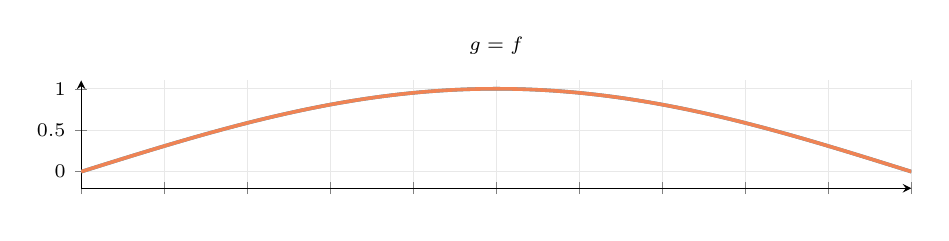
\begin{tikzpicture}
\begin{axis}[rep, width=\linewidth, height=2.95cm, xmin=0, xmax=1, ymin=-0.2, ymax=1.1, title={\scriptsize $g = f$}, xticklabels={}]
\addplot[sblue, line width=1.3pt, domain=0:1, samples=161] {sin(deg(pi*x))};
\addplot[sorange, line width=1.3pt, domain=0:1, samples=161] {sin(deg(pi*x))};
\end{axis}
\end{tikzpicture}

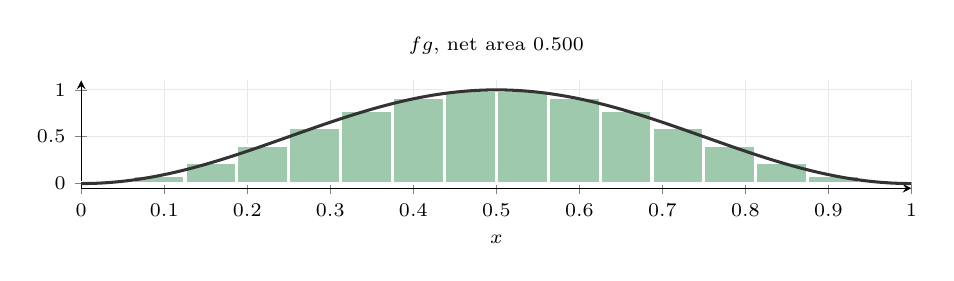
\begin{tikzpicture}
\begin{axis}[rep, width=\linewidth, height=2.95cm, xmin=0, xmax=1, ymin=-0.05, ymax=1.1, xlabel=$x$, title={\scriptsize $fg$, net area $0.500$}]
\stepfrom{2}{\addplot[ybar, bar width=0.0625, fill=sgreen!55, draw=white, samples at={0.03125,0.09375,0.15625,0.21875,0.28125,0.34375,0.40625,0.46875,0.53125,0.59375,0.65625,0.71875,0.78125,0.84375,0.90625,0.96875}] {max(sin(deg(pi*x))*sin(deg(pi*x)),0)};
\addplot[ybar, bar width=0.0625, fill=sred!55, draw=white, samples at={0.03125,0.09375,0.15625,0.21875,0.28125,0.34375,0.40625,0.46875,0.53125,0.59375,0.65625,0.71875,0.78125,0.84375,0.90625,0.96875}] {min(sin(deg(pi*x))*sin(deg(pi*x)),0)};
\addplot[ink, line width=1.1pt, domain=0:1, samples=161] {sin(deg(pi*x))*sin(deg(pi*x))};}
\end{axis}
\end{tikzpicture}
\end{columns}
\vspace{-2pt}
\[
\langle f, g\rangle = \int_0^1 f(x)\,g(x)\,dx \;\approx\; \frac{1}{16}\sum_{i=1}^{16} f(x_i)\,g(x_i)
\]
\note{
The uniform load $f=2$ produces the parabola $u=x(1-x)$.
Finding its closest three-sine sum requires an inner product.
For sampled functions, multiply matching values and weight them by the spacing.
As the spacing tends to zero, this Riemann sum becomes $\langle f,g\rangle=\int_0^1 fg\,dx$.

The product is positive where the functions have the same sign and negative where their signs differ.
The integral adds these signed contributions.
For $\sin(\pi x)$ and $\sin(2\pi x)$, reflection about mid-span changes the product's sign.
The contributions cancel, so the modes are orthogonal.

The first sine and the parabola are positive inside the interval.
Their product integrates to $4/\pi^3=0.129$.
The squared first sine integrates to $\tfrac12$, its squared $L^2$ norm.
The weighted sixteen-sample sums approximate these integrals as $0.000$, $0.129$, and $0.500$ to three digits.
}
\end{frame}

\begin{frame}{Minimizing squared error via orthogonal projection}
\begin{columns}[T]
\column{0.5\textwidth}
\begin{tikzpicture}
\begin{axis}[rep, height=5.2cm, xmin=0, xmax=1, ymin=0, ymax=0.32, xlabel=$x$, legend pos=south east]
\addplot[ink, dashed, line width=1.4pt] table[x=x, y=u]{data/parab.dat};
\addlegendentry{parabola}
\steponly{1}{3}{\addplot[sblue, line width=1.6pt, domain=0:1, samples=201] {0.20*sin(deg(pi*x)) + 0.00956*sin(deg(3*pi*x))}; \addlegendentry{$c_1 = 0.20$}}
\steponly{3}{3}{\addplot[sblue, line width=1.6pt, domain=0:1, samples=201] {0.258*sin(deg(pi*x)) + 0.00956*sin(deg(3*pi*x))}; \addlegendentry{$c_1 = 0.258$, the projection}
               \addplot[sorange, line width=1.6pt, domain=0:1, samples=201] {0.31*sin(deg(pi*x)) + 0.00956*sin(deg(3*pi*x))}; \addlegendentry{$c_1 = 0.31$}}
\end{axis}
\end{tikzpicture}
\column{0.5\textwidth}
\begin{tikzpicture}
\begin{axis}[rep, height=5.2cm, xmin=0.195, xmax=0.325, ymin=0, ymax=0.0024, xlabel=$c_1$, ylabel={\scriptsize $\|u - v\|_{L^2}^2$}, scaled y ticks=false, yticklabel style={/pgf/number format/fixed, /pgf/number format/precision=4}]
\addplot[ink, line width=1.3pt] table[x=c1, y=err2]{data/proj_err2.dat};
\steponly{1}{3}{\addplot[only marks, mark=*, mark size=3pt, sblue] coordinates {(0.20, 0.001685)};}
\steponly{3}{3}{\addplot[only marks, mark=*, mark size=3pt, sblue] coordinates {(0.258, 0.0000025)};
               \addplot[only marks, mark=*, mark size=3pt, sorange] coordinates {(0.31, 0.001354)};}
\end{axis}
\end{tikzpicture}
\end{columns}
\smallskip
\centering
\stepfrom{3}{\chip{$c_1 = 8/\pi^3 = 0.258$}{error $0.87$ percent}\quad\chip{$c_1 = 0.31$, twenty percent high}{error norm $23$ times larger}}
\hfill\live{coefficients-on-shapes}
\note{
Keep $c_2=0$ and $c_3=8/(27\pi^3)$ while varying $c_1$.
The squared $L^2$ error is a quadratic function of $c_1$.
Its derivative is $-2\langle u-v,\sin(\pi x)\rangle$.

At the minimum, the error is orthogonal to the first mode.
The coefficient is therefore $c_1=2\langle u,\sin(\pi x)\rangle=8/\pi^3=0.258$.
The resulting three-mode approximation has relative $L^2$ error $0.87$ percent.

Increasing $c_1$ by twenty percent changes it to approximately $0.31$.
The squared $L^2$ error increases from $2.5\times10^{-6}$ to $1.35\times10^{-3}$.
Its square root increases by a factor of $23$, although the curves appear similar at this plot scale.
}
\end{frame}

\begin{frame}{Uniqueness of the projection and the Pythagorean identity}
\begin{columns}
\column{0.5\textwidth}
\begin{center}
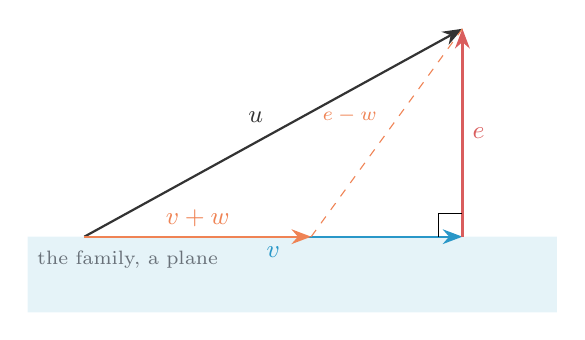
\begin{tikzpicture}[scale=1.2, >={Stealth[length=2.5mm]}, font=\small]
\coordinate (O) at (0,0);
\coordinate (V) at (4,0);
\coordinate (U) at (4,2.2);
\coordinate (W) at (2.4,0);
\fill[sblue!12] (O) -- (5,0) -- (5,-0.8) -- (-0.6,-0.8) -- (-0.6,0) -- cycle;
\node[muted, anchor=north west, font=\scriptsize] at (-0.6,-0.05) {the family, a plane};
\draw[->, ink, thick] (O) -- (U) node[midway, above left] {$u$};
\draw[->, sblue, thick] (O) -- (V) node[midway, below] {$v$};
\draw[->, sred, thick] (V) -- (U) node[midway, right] {$e$};
\stepfrom{2}{\draw[->, sorange, thick] (O) -- (W) node[midway, above] {$v + w$};
\draw[sorange, dashed] (W) -- (U) node[midway, above left, font=\scriptsize] {$e - w$};}
\draw (3.75,0) -- (3.75,0.25) -- (4,0.25);
\end{tikzpicture}
\end{center}
\column{0.5\textwidth}
\stepfrom{2}{\[
\|e - w\|^2 = \|e\|^2 + \|w\|^2
\]}
\stepfrom{3}{\[
\|u\|^2 = \|v\|^2 + \|e\|^2, \qquad 0.033333 = 0.033331 + 2.5 \times 10^{-6}
\]}
\end{columns}
\note{
Write the target as $u=v+e$, where $v$ belongs to the trial space and $e$ is orthogonal to it.
Any other trial function is $v+w$ for some $w$ in that space.
Its error is $e-w$.
Orthogonality gives $\|e-w\|^2=\|e\|^2+\|w\|^2$.

The additional term is nonnegative and vanishes only when $w=0$.
Thus $v$ is the unique closest trial function.
Taking $w=-v$ gives the Pythagorean identity $\|u\|^2=\|v\|^2+\|e\|^2$.
For the parabola, the squared $L^2$ norms are $0.033333$ and $0.033331$, leaving squared error $2.5\times10^{-6}$ and relative error $0.87$ percent.
}
\end{frame}

\begin{frame}{The projection theorem}
\begin{block}{Projection theorem}
For each target in an inner-product space, a finite-dimensional linear subspace has a unique closest member.
Its error is orthogonal to that subspace.
\end{block}
\bigskip
\[
\langle u - v, \phi_j\rangle = 0 \quad \text{for every shape } \phi_j, \qquad c_k = \frac{\langle u, \phi_k\rangle}{\langle \phi_k, \phi_k\rangle} \text{ when the shapes are orthogonal.}
\]
\note{
Orthogonality gives a linear system for the projection coefficients.
An orthogonal basis reduces this system to one division per coefficient.
Fourier coefficients are obtained this way in the $L^2$ inner product.

The projection theorem guarantees a unique closest element in a closed linear subspace of a Hilbert space.
Every finite-dimensional linear subspace is closed.
A nonlinear family need not have a unique closest element, as the unit circle and the origin demonstrate.
How does changing the inner product change the projection?
}
\end{frame}

\begin{frame}{Projection in the $L^2$ and energy inner products}
\begin{columns}
\column{0.7\textwidth}
\begin{tikzpicture}
\begin{axis}[rep, height=6.2cm, xmin=0, xmax=1, ymin=0, ymax=0.3, xlabel=$x$, legend pos=south east]
\addplot[ink, dashed, line width=1.4pt] table[x=x, y=u]{data/parab.dat};
\addlegendentry{parabola}
\addplot[sblue, line width=1.6pt, mark=*, mark size=2pt] table[x=x, y=v]{data/seg_energy.dat};
\addlegendentry{closest in energy}
\stepfrom{2}{\addplot[sorange, line width=1.6pt, mark=*, mark size=2pt] table[x=x, y=v]{data/seg_l2.dat};
          \addlegendentry{closest in $L^2$}}
\end{axis}
\end{tikzpicture}
\column{0.3\textwidth}
\chip{closest in energy, heights}{$0.1875$, $0.25$, $0.1875$}\\[4pt]
\stepfrom{2}{\chip{closest in $L^2$, heights}{$0.2009$, $0.2589$, $0.2009$}\\[4pt]
\chip{$L^2$ error, $L^2$ against energy}{$3.3$ against $6.3$ percent}\\[4pt]
\chip{relative slope error, $L^2$ against energy}{$26.0$ against $25.0$ percent}}
\end{columns}
\note{
Keep the parabola and use pinned piecewise-linear functions with breaks at $0.25$, $0.5$, and $0.75$.
The energy inner product is $\int_0^1 f'g'\,dx$ on the pinned space.
Its projection takes the nodal values $0.1875$, $0.25$, and $0.1875$.
The slope error integrates to zero on each segment.

The $L^2$ projection instead takes the nodal values $0.2009$, $0.2589$, and $0.2009$.
It reduces integrated value error by allowing nonzero error at the nodes.
Each projection minimizes its own norm over the same trial space.

For the Dirichlet sine basis, the two projections coincide.
Integration by parts gives $\langle u',\phi_k'\rangle=(k\pi)^2\langle u,\phi_k\rangle$.
The basis norm has the same factor, which cancels in the coefficient formula.
Being orthogonal in both inner products would not by itself make the projections equal.
}
\end{frame}

%========================================================================================
\repsection{Bases}{Changing the basis}

\begin{frame}{Five fixed families of shapes}
\begin{center}
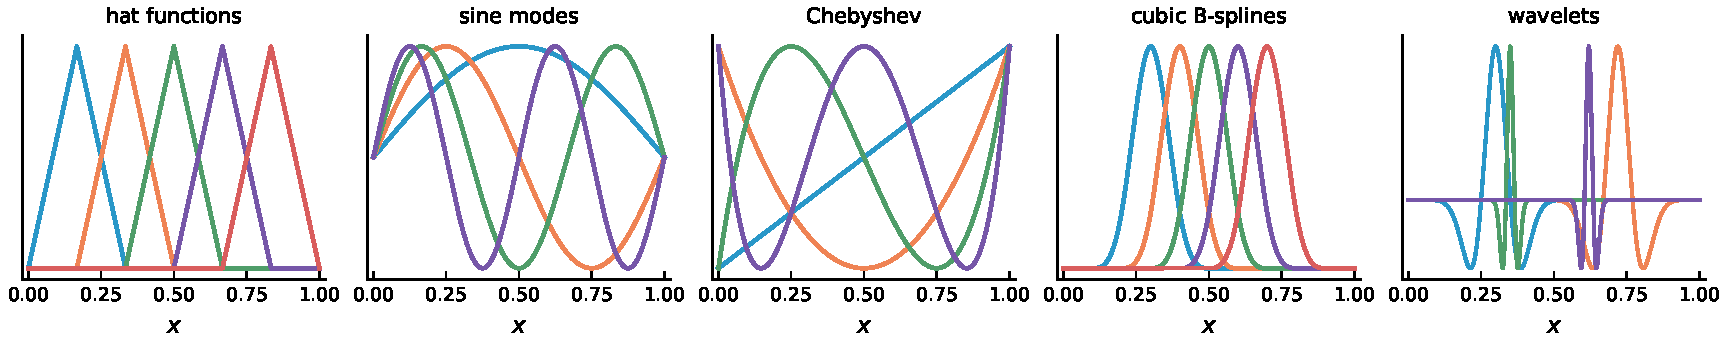
\includegraphics[width=\textwidth]{figs/rep-basis-gallery}
\end{center}
\centering
\chip{local}{hats, one per node}\quad\chip{global}{sine modes, Chebyshev polynomials}\quad\chip{smooth and local}{cubic B-splines}\quad\chip{local in position and scale}{wavelets}
\note{
The sine modes are one possible basis.
Hat functions are supported on the segments adjacent to their nodes.
Sine modes and Chebyshev polynomials extend across the interval.
Cubic B-splines combine local support with greater smoothness.

A coefficient changes the function only where its basis function is nonzero.
Local bases therefore permit local changes, while global bases couple distant locations.
Wavelets also distinguish scales of variation.
The point-load displacement shows how matching the basis to a corner reduces the number of coefficients.
}
\end{frame}

\begin{frame}{Piecewise-linear interpolation as a hat-function expansion}
\begin{columns}
\column{0.7\textwidth}
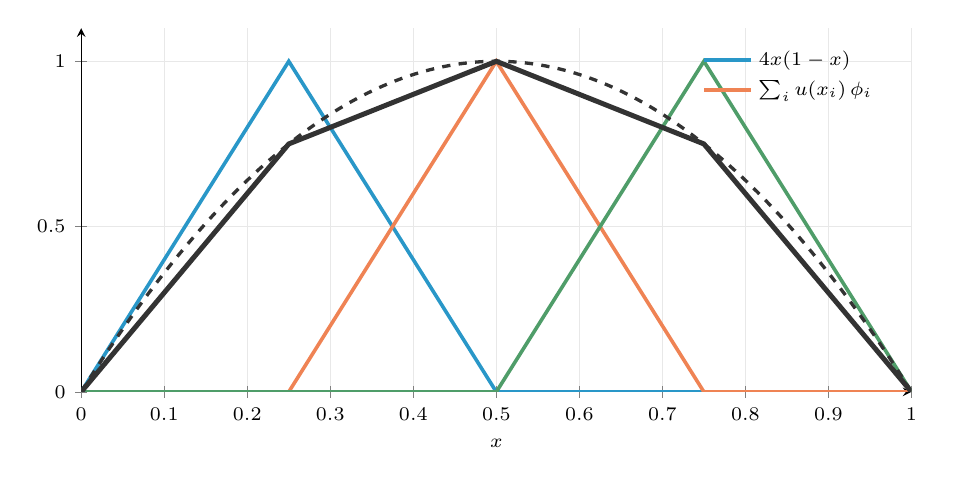
\begin{tikzpicture}
\begin{axis}[rep, height=6.2cm, xmin=0, xmax=1, ymin=0, ymax=1.1, xlabel=$x$, legend pos=north east]
\addplot[sblue, line width=1.3pt, domain=0:1, samples=201] {max(0, 1 - abs(x-0.25)/0.25)};
\stepfrom{2}{\addplot[sorange, line width=1.3pt, domain=0:1, samples=201] {max(0, 1 - abs(x-0.5)/0.25)};}
\stepfrom{3}{\addplot[sgreen, line width=1.3pt, domain=0:1, samples=201] {max(0, 1 - abs(x-0.75)/0.25)};}
\stepfrom{4}{\addplot[ink, dashed, line width=1.2pt, domain=0:1, samples=201] {4*x*(1-x)};
          \addlegendentry{$4x(1-x)$}
          \addplot[ink, line width=1.8pt, domain=0:1, samples=201] {0.75*max(0, 1 - abs(x-0.25)/0.25) + 1.0*max(0, 1 - abs(x-0.5)/0.25) + 0.75*max(0, 1 - abs(x-0.75)/0.25)};
          \addlegendentry{$\sum_i u(x_i)\,\phi_i$}}
\end{axis}
\end{tikzpicture}
\column{0.3\textwidth}
\stepfrom{4}{\[
u_h(x) = \sum_i u(x_i)\,\phi_i(x)
\]}
\end{columns}
\note{
The piecewise-linear interpolant can be written in a basis.
At each interior node, define a hat that equals one there, zero at the other nodes, and is linear between nodes.
The hats are linearly independent and span the pinned piecewise-linear functions on this grid.

Weighting each hat by its nodal reading gives $u_h(x)=\sum_i u(x_i)\phi_i(x)$.
At a node, every term except that node's hat is zero.
The sum therefore reproduces the readings and connects them by straight segments.
On this one-dimensional pinned string, it is also the energy projection.
}
\end{frame}

\begin{frame}{Representing a kink in the hat basis and the sine basis}
\begin{columns}
\column{0.7\textwidth}
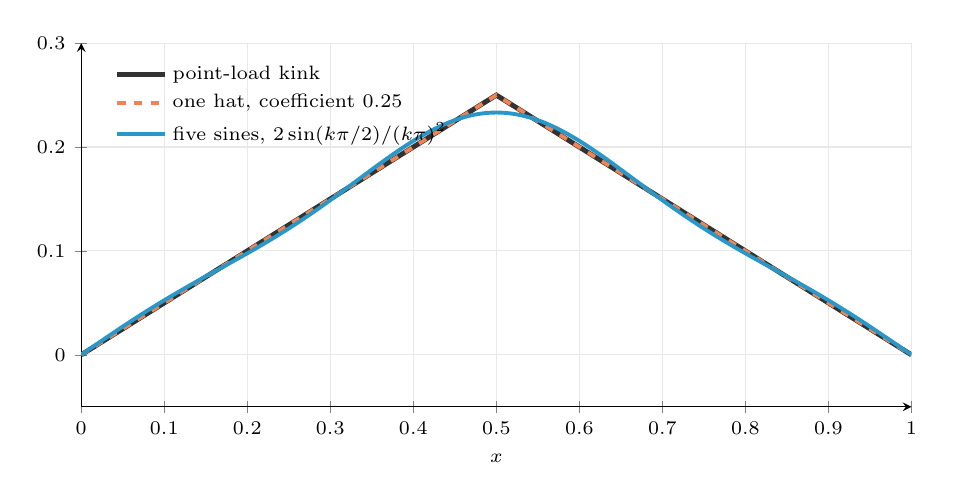
\begin{tikzpicture}
\begin{axis}[rep, height=6.2cm, xmin=0, xmax=1, ymin=-0.05, ymax=0.3, xlabel=$x$, legend pos=north west]
\addplot[ink, line width=1.8pt, domain=0:1, samples=201] {0.5*min(x, 1-x)};
\addlegendentry{point-load kink}
\stepfrom{2}{\addplot[sorange, line width=1.4pt, dashed, domain=0:1, samples=201] {0.25*max(0, 1 - abs(x-0.5)/0.5)};
          \addlegendentry{one hat, coefficient $0.25$}}
\stepfrom{3}{\addplot[sblue, line width=1.4pt, domain=0:1, samples=301] {0.2026*sin(deg(pi*x)) - 0.0225*sin(deg(3*pi*x)) + 0.0081*sin(deg(5*pi*x))};
          \addlegendentry{five sines, $2\sin(k\pi/2)/(k\pi)^2$}}
\end{axis}
\end{tikzpicture}
\column{0.3\textwidth}
\stepfrom{2}{\chip{one hat on the corner}{one number, $0.25$, no error}\\[4pt]
\chip{three hats, five stations}{$0.125$, $0.25$, $0.125$, no error}\\[4pt]}
\stepfrom{3}{\chip{relative $L^2$ error, three and thirty-three sines}{$4.8$ and $0.20$ percent}}
\vfill
\live{coefficients-on-shapes}
\end{columns}
\note{
The point-load corner matches a hat with its node at mid-span.
Multiplying that hat by $0.25$ reproduces the displacement without error.
On the five-station grid, the same displacement has hat coefficients $0.125$, $0.25$, and $0.125$.

Its sine representation instead needs the infinite sequence $c_k=2\sin(k\pi/2)/(k\pi)^2$.
Three modes leave relative $L^2$ error $4.8$ percent, and thirty-three leave $0.20$ percent.
A basis with the correct corner can therefore represent this displacement with fewer coefficients than smooth sine modes.
This advantage depends on placing the hat node at the corner.
}
\end{frame}

\begin{frame}{Galerkin's method with hat functions}
\begin{columns}
\column{0.52\textwidth}
\begin{tikzpicture}
\begin{axis}[rep, height=5.2cm, xmin=0, xmax=1, ymin=-0.2, ymax=1.35, xlabel=$x$, ylabel=$u(x)$, legend pos=north east]
\addplot[ink, dashed, line width=1.4pt] table[x=x, y=u]{data/string.dat};
\addlegendentry{exact $u$}
\stepfrom{2}{\addplot[sblue, line width=1.6pt, mark=*, mark size=2pt] table[x=x, y=uh]{data/galerkin4.dat};
          \addlegendentry{Galerkin $u_h$, four elements}}
\end{axis}
\end{tikzpicture}
\column{0.48\textwidth}
\small
\[
\int_0^1 u_h'\,\phi_i'\,dx = \int_0^1 f\,\phi_i\,dx \quad\text{for every hat } \phi_i
\]
\[
\mathbf{K}\mathbf{u} = \mathbf{F}, \qquad K_{ii} = \frac{2}{h}, \quad K_{i,i\pm1} = -\frac{1}{h}
\]
\stepfrom{2}{\chip{largest nodal deviation, $4$ to $16$ elements}{$4.4 \times 10^{-16}$}\\[4pt]}
\stepfrom{3}{\chip{error slopes on log axes, $L^2$ and energy}{$2.00$ and $1.00$}}
\end{columns}
\note{
Galerkin's method determines the hat coefficients from the equation rather than from displacement readings.
Hats lack classical second derivatives at their nodes, so they cannot satisfy $-u_h''=f$ pointwise there.
Integration by parts gives the weak equation $\int u_h'v'\,dx=\int fv\,dx$.
This equation requires only square-integrable first derivatives.

Testing against each hat gives $\mathbf{K}\mathbf{u}=\mathbf{F}$.
On the uniform grid, the hat slopes give $K_{ii}=2/h$ and $K_{i,i\pm1}=-1/h$.
The error is orthogonal to the hat space in the energy inner product, so this solution is its energy projection.

For this one-dimensional constant-coefficient equation with exact load integration, the Galerkin solution reproduces the exact nodal values.
The Green's function centered at each grid node is a tent in the hat space, which proves the nodal equality.
The measured largest nodal deviation is $4.4\times10^{-16}$ over four, eight, and sixteen elements.
For the smooth test displacement, the $L^2$ and energy errors decrease as $h^2$ and $h$, respectively.
The measured log-log slopes are $2.00$ and $1.00$.
}
\end{frame}

\begin{frame}{Convergence of hat interpolation for continuous and discontinuous functions}
\begin{columns}[T]
\column{0.33\textwidth}
\begin{tikzpicture}
\begin{axis}[rep, height=3.7cm, xmin=0, xmax=1, ymin=-0.3, ymax=1.35, xlabel=$x$, title={\scriptsize the string, five stations}]
\stepfrom{2}{\foreach \i in {1,...,3} {\addplot[muted, dashed, line width=0.8pt, forget plot] table[x=x, y=h\i]{data/hats_string5.dat};}}
\addplot[ink, line width=1.6pt] table[x=x, y=f]{data/hats_string5.dat};
\stepfrom{2}{\addplot[sblue, line width=1.6pt] table[x=x, y=v]{data/hats_string5.dat};}
\addplot[only marks, mark=*, mark size=2pt, sred] table[x=x, y=y]{data/hats_string5_nodes.dat};
\end{axis}
\end{tikzpicture}
\column{0.33\textwidth}
\begin{tikzpicture}
\begin{axis}[rep, height=3.7cm, xmin=0, xmax=1, ymin=-0.6, ymax=1.3, xlabel=$x$, title={\scriptsize a bump, seventeen stations}]
\stepfrom{3}{\foreach \i in {1,...,15} {\addplot[muted, dashed, line width=0.6pt, forget plot] table[x=x, y=h\i]{data/hats_bump17.dat};}
\addplot[ink, line width=1.6pt] table[x=x, y=f]{data/hats_bump17.dat};
\addplot[sblue, line width=1.6pt] table[x=x, y=v]{data/hats_bump17.dat};
\addplot[only marks, mark=*, mark size=1.4pt, sred] table[x=x, y=y]{data/hats_bump17_nodes.dat};}
\end{axis}
\end{tikzpicture}
\column{0.33\textwidth}
\begin{tikzpicture}
\begin{axis}[rep, height=3.7cm, xmin=0, xmax=1, ymin=-0.15, ymax=1.25, xlabel=$x$, title={\scriptsize a square pulse, seventeen stations}]
\stepfrom{4}{\foreach \i in {5,...,11} {\addplot[muted, dashed, line width=0.7pt, forget plot] table[x=x, y=h\i]{data/hats_pulse17.dat};}
\addplot[ink, line width=1.6pt] table[x=x, y=f]{data/hats_pulse17.dat};
\addplot[sblue, line width=1.6pt] table[x=x, y=v]{data/hats_pulse17.dat};
\addplot[only marks, mark=*, mark size=1.6pt, sred] table[x=x, y=y]{data/hats_pulse17_nodes.dat};}
\end{axis}
\end{tikzpicture}
\end{columns}
\[
u_h(x) = \sum_i u(x_i)\,\phi_i(x), \qquad \phi_i(x_j) = \begin{cases} 1 & i = j \\ 0 & i \ne j \end{cases}
\]
\centering
\stepfrom{2}{\chip{string, largest gap at $5$, $17$, $33$ stations}{$20.1$, $1.6$, $0.4$ percent}}\quad
\stepfrom{3}{\chip{bump, largest gap at $9$, $33$, $65$ stations}{$13.4$, $2.1$, $0.5$ percent}}\quad
\stepfrom{4}{\chip{pulse, largest gap and RMS gap at $17$}{$80$ and $23.3$ percent}}
\hfill\live{hat-functions-as-a-basis}
\note{
Refining the hat grid approximates every continuous function on the interval uniformly.
On each segment, the interpolant lies between its endpoint readings.
Uniform continuity bounds the error by the function's variation over distances at most $h$.
For a twice continuously differentiable function with $|u''|\le M$, the sharper bound is $Mh^2/8$.

The smooth string displacement has relative sup errors $20.1$, $1.6$, and $0.4$ percent at five, seventeen, and thirty-three stations.
The narrower bump requires smaller spacing.
Its relative sup errors are $13.4$, $2.1$, and $0.5$ percent at nine, thirty-three, and sixty-five stations.

The square pulse has jumps, so continuous hat sums cannot converge to it in the sup norm.
Every continuous approximation has sup error at least half the jump magnitude.
For the sampled interpolants shown, the relative sup error stays between $60$ and $80$ percent.
Their relative $L^2$ error still decreases from $23.3$ percent at seventeen stations to $11.6$ percent at sixty-five.
Thus convergence depends on both the target's regularity and the chosen norm.
}
\end{frame}

\begin{frame}{Decay rates of sine coefficients}
\begin{columns}
\column{0.7\textwidth}
\begin{figure}
\centering
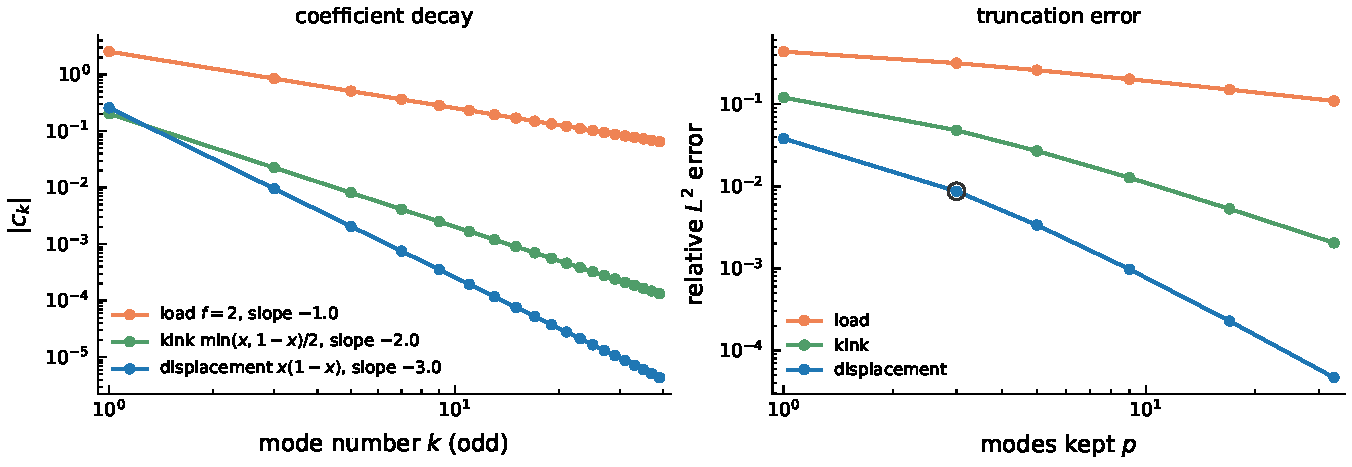
\includegraphics[width=\textwidth]{figs/rep-coefficients}
\end{figure}
\column{0.3\textwidth}
\chip{load $f = 2$, odd $k$}{$|c_k| = 8/(k\pi)$, slope $-1.0$}\\[4pt]
\chip{kink, odd $k$}{$|c_k| = 2/(k\pi)^2$, slope $-2.0$}\\[4pt]
\chip{parabola, odd $k$}{$|c_k| = 8/(k\pi)^3$, slope $-3.0$}
\end{columns}
\note{
The uniform load $f=2$ has sine coefficients $8/(k\pi)$ for odd $k$ and zero for even $k$.
The point-load displacement has coefficients $2\sin(k\pi/2)/(k\pi)^2$.
The parabola has coefficients $8/(k\pi)^3$ for odd $k$.
The equation $-u''=f$ divides each load coefficient by $(k\pi)^2$.

The nonzero magnitudes therefore decay as $1/k$, $1/k^2$, and $1/k^3$ in these examples.
The load's odd periodic continuation jumps at the endpoints.
The corner is continuous but has a slope jump, while the parabola's odd continuation has a continuous first derivative.
Coefficient decay depends on the regularity of this continuation, including the boundary behavior.

One mode leaves relative $L^2$ error $44$ percent for the uniform load.
Thirty-three modes still leave $11$ percent.
The slow decay reflects the jumps in the continuation, rather than a pointwise endpoint error alone.
What does a truncated series do near a jump?
}
\end{frame}

\begin{frame}{The Gibbs phenomenon at a jump}
\begin{columns}
\column{0.7\textwidth}
\begin{tikzpicture}
\begin{axis}[rep, height=6.2cm, xmin=0.3, xmax=0.7, ymin=-0.2, ymax=1.2, xlabel=$x$, legend pos=south east]
\addplot[ink, dashed, line width=1.2pt] coordinates {(0.3,0) (0.5,0) (0.5,1) (0.7,1)};
\addlegendentry{step}
\addplot[sblue!50, line width=1.2pt] table[x=x, y=s]{data/gibbs9.dat};
\addlegendentry{$N = 9$}
\stepfrom{2}{\addplot[sblue!80, line width=1.2pt] table[x=x, y=s]{data/gibbs33.dat};
          \addlegendentry{$N = 33$}}
\stepfrom{3}{\addplot[sblue, line width=1.2pt] table[x=x, y=s]{data/gibbs129.dat};
          \addlegendentry{$N = 129$}}
\addplot[sred, dashed, line width=0.8pt] coordinates {(0.3,1.0895) (0.7,1.0895)};
\end{axis}
\end{tikzpicture}
\column{0.3\textwidth}
\chip{overshoot, $N = 9$}{$0.091$}\\[4pt]
\stepfrom{2}{\chip{overshoot, $N = 33$}{$0.090$}\\[4pt]}
\stepfrom{3}{\chip{overshoot, $N = 129$}{$0.089$, toward $0.0895$}}
\end{columns}
\note{
The truncated sine series overshoots the step near its jump.
Increasing the number of modes narrows the oscillating region.
The overshoot tends to about $0.0895$ times the jump magnitude.

This nonvanishing overshoot is the Gibbs phenomenon.
The series does not converge in the sup norm.
It does converge in $L^2$ because the region of large error shrinks.
Convergence in one norm therefore does not imply convergence in another.
}
\end{frame}

\begin{frame}{Conditioning of the Gram matrix for nearly parallel shapes}
\begin{columns}
\column{0.5\textwidth}
\begin{center}
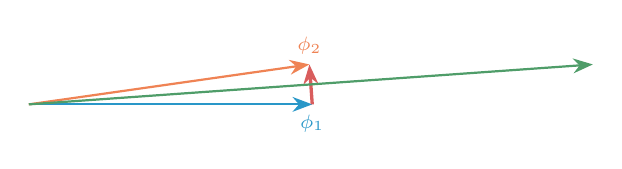
\begin{tikzpicture}[scale=0.9, >={Stealth[length=2.5mm]}, font=\small]
\coordinate (O) at (0,0);
\draw[->, sblue, thick] (O) -- (4,0) node[below, font=\scriptsize] {$\phi_1$};
\draw[->, sorange, thick] (O) -- ({4*cos(8.1)},{4*sin(8.1)}) node[above, font=\scriptsize] {$\phi_2$};
\stepfrom{2}{\draw[->, sred, very thick] (4,0) -- ({4*cos(8.1)},{4*sin(8.1)});}
\stepfrom{3}{\draw[->, sgreen, thick] (O) -- ({4+4*cos(8.1)},{4*sin(8.1)});}
\end{tikzpicture}

\scriptsize
\stepfrom{2}{\textcolor{sred}{$\phi_2 - \phi_1$, length $0.14$}}\quad\stepfrom{3}{\textcolor{sgreen}{$\phi_1 + \phi_2$, length $1.995$}}
\end{center}
\[
\mathbf{G} = \begin{pmatrix} 1 & \rho \\ \rho & 1\end{pmatrix}, \qquad \rho = 0.99, \qquad \cond \mathbf{G} = \frac{1+\rho}{1-\rho} = 199
\]
\column{0.5\textwidth}
\stepfrom{2}{\chip{add $0.1(\phi_1 - \phi_2)$}{target moves $0.014$, coefficients $0.1$ and $-0.1$}\\[4pt]}
\stepfrom{3}{\chip{add $0.1(\phi_1 + \phi_2)$}{target moves $0.2$, fourteen times more}\\[4pt]
\chip{$\sqrt{199}$}{$14.1$}\\[4pt]
\chip{neighboring hats}{$\rho = 1/4$}\\[4pt]
\chip{five Gaussian bumps a third of a width apart}{$\cond \mathbf{G} = 2.4$ million}}
\end{columns}
\note{
Consider two functions of norm one with inner product $\rho=0.99$.
Their Gram matrix has eigenvalues $1+\rho$ and $1-\rho$.
Its condition number is $(1+\rho)/(1-\rho)=199$.

The difference of the functions has norm $\sqrt{2-2\rho}=0.14$.
Adding $0.1(\phi_1-\phi_2)$ changes the target by norm $0.014$ while changing the coefficients by $0.1$ and $-0.1$.
The same coefficient magnitudes with equal signs change the target by norm $0.2$.
The ratio is $\sqrt{199}=14.1$, so coefficient recovery is sensitive along the difference direction.

Overlap alone does not imply severe ill-conditioning.
Neighboring normalized hats have inner product $1/4$.
The five Gaussian bumps shown, separated by one third of their width, instead give Gram condition number $2.4$ million.
}
\end{frame}

%========================================================================================
\repsection{Convergence}{Convergence, density, and completeness}

\begin{frame}{Bernstein basis polynomials of degree $0$ to $5$}
\begin{center}
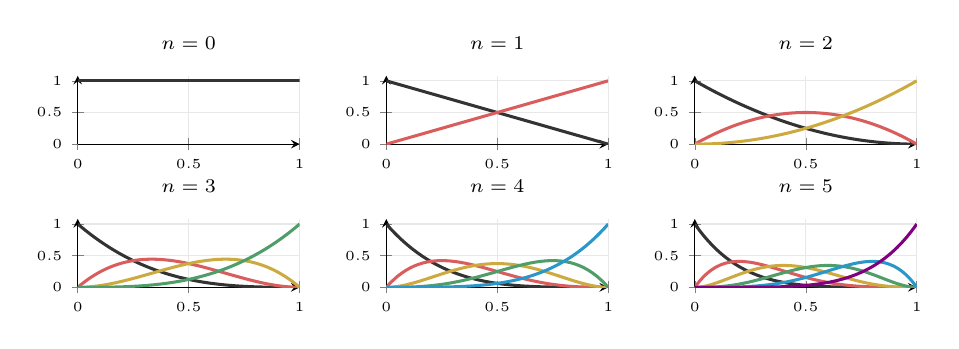
\begin{tikzpicture}
\begin{groupplot}[group style={group size=3 by 2, horizontal sep=1.1cm, vertical sep=0.95cm}, width=4.4cm, height=2.45cm, xmin=0, xmax=1, ymin=0, ymax=1.08, axis lines=left, grid=major, grid style={gray!18}, tick label style={font=\tiny}, xtick={0,0.5,1}, ytick={0,0.5,1}, clip mode=individual]
\nextgroupplot[title={\scriptsize $n = 0$}]
\addplot[ink, line width=1.1pt, domain=0:1, samples=81] {factorial(0)/(factorial(0)*factorial(0-0))*x^0*(1-x)^(0-0)};
\nextgroupplot[title={\scriptsize $n = 1$}]
\addplot[ink, line width=1.1pt, domain=0:1, samples=81] {factorial(1)/(factorial(0)*factorial(1-0))*x^0*(1-x)^(1-0)};
\addplot[sred, line width=1.1pt, domain=0:1, samples=81] {factorial(1)/(factorial(1)*factorial(1-1))*x^1*(1-x)^(1-1)};
\nextgroupplot[title={\scriptsize $n = 2$}]
\addplot[ink, line width=1.1pt, domain=0:1, samples=81] {factorial(2)/(factorial(0)*factorial(2-0))*x^0*(1-x)^(2-0)};
\addplot[sred, line width=1.1pt, domain=0:1, samples=81] {factorial(2)/(factorial(1)*factorial(2-1))*x^1*(1-x)^(2-1)};
\addplot[syellow!85!black, line width=1.1pt, domain=0:1, samples=81] {factorial(2)/(factorial(2)*factorial(2-2))*x^2*(1-x)^(2-2)};
\nextgroupplot[title={\scriptsize $n = 3$}]
\addplot[ink, line width=1.1pt, domain=0:1, samples=81] {factorial(3)/(factorial(0)*factorial(3-0))*x^0*(1-x)^(3-0)};
\addplot[sred, line width=1.1pt, domain=0:1, samples=81] {factorial(3)/(factorial(1)*factorial(3-1))*x^1*(1-x)^(3-1)};
\addplot[syellow!85!black, line width=1.1pt, domain=0:1, samples=81] {factorial(3)/(factorial(2)*factorial(3-2))*x^2*(1-x)^(3-2)};
\addplot[sgreen, line width=1.1pt, domain=0:1, samples=81] {factorial(3)/(factorial(3)*factorial(3-3))*x^3*(1-x)^(3-3)};
\nextgroupplot[title={\scriptsize $n = 4$}]
\addplot[ink, line width=1.1pt, domain=0:1, samples=81] {factorial(4)/(factorial(0)*factorial(4-0))*x^0*(1-x)^(4-0)};
\addplot[sred, line width=1.1pt, domain=0:1, samples=81] {factorial(4)/(factorial(1)*factorial(4-1))*x^1*(1-x)^(4-1)};
\addplot[syellow!85!black, line width=1.1pt, domain=0:1, samples=81] {factorial(4)/(factorial(2)*factorial(4-2))*x^2*(1-x)^(4-2)};
\addplot[sgreen, line width=1.1pt, domain=0:1, samples=81] {factorial(4)/(factorial(3)*factorial(4-3))*x^3*(1-x)^(4-3)};
\addplot[sblue, line width=1.1pt, domain=0:1, samples=81] {factorial(4)/(factorial(4)*factorial(4-4))*x^4*(1-x)^(4-4)};
\nextgroupplot[title={\scriptsize $n = 5$}]
\addplot[ink, line width=1.1pt, domain=0:1, samples=81] {factorial(5)/(factorial(0)*factorial(5-0))*x^0*(1-x)^(5-0)};
\addplot[sred, line width=1.1pt, domain=0:1, samples=81] {factorial(5)/(factorial(1)*factorial(5-1))*x^1*(1-x)^(5-1)};
\addplot[syellow!85!black, line width=1.1pt, domain=0:1, samples=81] {factorial(5)/(factorial(2)*factorial(5-2))*x^2*(1-x)^(5-2)};
\addplot[sgreen, line width=1.1pt, domain=0:1, samples=81] {factorial(5)/(factorial(3)*factorial(5-3))*x^3*(1-x)^(5-3)};
\addplot[sblue, line width=1.1pt, domain=0:1, samples=81] {factorial(5)/(factorial(4)*factorial(5-4))*x^4*(1-x)^(5-4)};
\addplot[violet, line width=1.1pt, domain=0:1, samples=81] {factorial(5)/(factorial(5)*factorial(5-5))*x^5*(1-x)^(5-5)};
\end{groupplot}
\end{tikzpicture}
\end{center}
\vspace{-6pt}
\[
B_{i,n}(t) = \binom{n}{i} t^i (1-t)^{n-i}, \qquad \sum_{i=0}^{n} B_{i,n}(t) = 1, \qquad B_{i,n}(t) \ge 0
\]
{\centering\scriptsize $B_{i,n}(t)$ is the probability of exactly $i$ heads in $n$ flips of a coin that lands heads with probability $t$\par}
\note{
For $n$ independent coin flips with head probability $t$, the probability of $i$ heads is $\binom ni t^i(1-t)^{n-i}$.
The factor $\binom ni$ counts the possible orders of heads and tails.
As a function of $t$, this probability is the Bernstein basis polynomial $B_{i,n}(t)$.
The degree-zero basis is the constant one.

The basis polynomials are nonnegative and sum to one at every $t$.
For $n>0$, the interior members peak at $t=i/n$, while the endpoint members peak at zero and one.
The identity $B_{i,n}(t)=B_{n-i,n}(1-t)$ pairs the basis functions by reflection.

A sum $\sum_i\beta_iB_{i,n}(t)$ is therefore a weighted average of the coefficients.
It stays between their minimum and maximum and takes the endpoint values $\beta_0$ and $\beta_n$.
Using vector coefficients gives the B\'ezier curves used in vector graphics.
Choosing the coefficients as function samples gives Bernstein's approximation construction.
}
\end{frame}

\begin{frame}{Bernstein polynomials for the string displacement}
\begin{columns}
\column{0.66\textwidth}
\begin{tikzpicture}
\begin{axis}[rep, height=4.6cm, xmin=0, xmax=1, ymin=-0.1, ymax=1.35, xlabel=$x$, ylabel=$u(x)$, legend pos=north east]
\addplot[ink, dashed, line width=1.4pt] table[x=x, y=u]{data/bern_disp8.dat};
\addlegendentry{displacement}
\addplot[only marks, mark=*, mark size=1.8pt, sred] table[x=t, y=r]{data/bern_disp8_probe.dat};
\addlegendentry{readings $u(k/8)$}
\stepfrom{3}{\foreach \k in {0,...,8} {\addplot[muted, dashed, line width=0.7pt, forget plot] table[x=x, y=w\k]{data/bern_disp8.dat};}
          \addplot[sblue, line width=1.8pt] table[x=x, y=B]{data/bern_disp8.dat};
          \addlegendentry{$B_8 u$, the sum of the gray curves}}
\stepfrom{2}{\addplot[sred, dashed, line width=0.8pt, forget plot] coordinates {(0.25,-0.1) (0.25,1.35)};}
\end{axis}
\end{tikzpicture}
\begin{tikzpicture}
\begin{axis}[rep, height=2.8cm, xmin=0, xmax=1, ymin=0, ymax=0.35, xlabel={$k/8$}, ylabel={\scriptsize $P(k)$}, title={\scriptsize probability of $k$ heads in $8$ coins, $x = 0.25$}]
\stepfrom{2}{\addplot[ybar, bar width=6pt, fill=sblue!60, draw=none] table[x=t, y=p]{data/bern_disp8_probe.dat};}
\end{axis}
\end{tikzpicture}
\column{0.34\textwidth}
\small
\[
B_n u(x) = \sum_{k=0}^{n} u\!\left(\tfrac{k}{n}\right) b_{k,n}(x)
\]
\[
b_{k,n}(x) = \tbinom{n}{k} x^k (1-x)^{n-k}
\]
\stepfrom{2}{\chip{$B_8 u(0.25)$, the weighted average}{$0.810$ against $u(0.25) = 1.107$}\\[4pt]}
\stepfrom{3}{\chip{largest gap, $n = 8$, $32$, $128$}{$0.30$, $0.091$, $0.024$}\\[4pt]
\chip{Voronovskaya, large $n$}{$3.18/n$}}
\end{columns}
\note{
Take the displacement readings at $k/8$ for $k=0,\ldots,8$.
At $x=0.25$, weight each reading by the probability of $k$ heads in eight flips with head probability $0.25$.
The weights are nonnegative and sum to one.
Their weighted average is $0.810$, compared with the displacement value $1.107$.

At general $x$, this average is $B_nu(x)=\mathbb{E}[u(X/n)]$, where $X$ is binomial with parameters $n$ and $x$.
The sampled position $X/n$ has mean $x$ and variance $x(1-x)/n$.
Increasing $n$ concentrates the sampled positions near the evaluation point.

For a smooth displacement, a Taylor expansion explains the error.
The linear term averages to zero because $\mathbb{E}[X/n-x]=0$, even though the distribution is generally asymmetric.
The leading quadratic term is $x(1-x)u''(x)/(2n)$.
For this displacement, the sup error is $0.30$, $0.091$, and $0.024$ at $n=8$, $32$, and $128$, approaching the predicted $3.18/n$.

No finite-degree polynomial equals this nonpolynomial displacement.
Its three-sine representation is exact, whereas its Bernstein representation converges as the degree increases.
At a corner, the Taylor argument changes.
How does that change the rate?
}
\end{frame}

\begin{frame}{Approximating a corner with Bernstein polynomials}
\begin{columns}
\column{0.7\textwidth}
\begin{tikzpicture}
\begin{axis}[rep, height=6.2cm, xmin=0, xmax=1, ymin=0, ymax=1.05, xlabel=$x$, legend pos=north east]
\addplot[sblue, line width=1.3pt] table[x=x, y=h0]{data/hills2.dat};
\addlegendentry{$(1-x)^2$}
\addplot[sorange, line width=1.3pt] table[x=x, y=h1]{data/hills2.dat};
\addlegendentry{$2x(1-x)$}
\addplot[sgreen, line width=1.3pt] table[x=x, y=h2]{data/hills2.dat};
\addlegendentry{$x^2$}
\stepfrom{2}{\addplot[ink, dashed, line width=1.2pt] table[x=x, y=f]{data/bern2.dat};
          \addlegendentry{$|x - \tfrac12|$}
          \addplot[ink, line width=1.8pt] table[x=x, y=B]{data/bern2.dat};
          \addlegendentry{$B_2 f$}
          \addplot[only marks, mark=*, sred, mark size=2.4pt] coordinates {(0.5, 0.25)};}
\end{axis}
\end{tikzpicture}
\column{0.3\textwidth}
\chip{Bernstein basis weights at mid-span}{$\tfrac14$, $\tfrac12$, $\tfrac14$}\\[4pt]
\stepfrom{2}{\chip{readings of $|x - \tfrac12|$ at $0$, $\tfrac12$, $1$}{$\tfrac12$, $0$, $\tfrac12$}\\[4pt]
\chip{$B_2 f$ at the corner}{$\tfrac14$ where $f = 0$}}
\end{columns}
\note{
Consider the corner function $f(x)=|x-\tfrac12|$.
Its readings at $0$, $\tfrac12$, and $1$ are $\tfrac12$, $0$, and $\tfrac12$.
These are the coefficients of its degree-two Bernstein approximation.

At mid-span, the basis weights are $\tfrac14$, $\tfrac12$, and $\tfrac14$.
The weighted sum is therefore $\tfrac14$, although the corner value is zero.
Every sample away from the corner is larger than its value at the corner.
A positive average of these samples gives a positive approximation error there.
}
\end{frame}

\begin{frame}{Convergence rate of Bernstein polynomials}
\begin{columns}
\column{0.7\textwidth}
\begin{tikzpicture}
\begin{axis}[rep, height=5.6cm, xmin=0, xmax=1, ymin=0, ymax=0.6, xlabel=$x$, legend pos=north east]
\addplot[ink, dashed, line width=1.2pt] table[x=x, y=f]{data/bern2.dat};
\addlegendentry{$|x - \tfrac12|$}
\steponly{1}{3}{\addplot[sblue!50, line width=1.8pt] table[x=x, y=B]{data/bern2.dat};
         \addlegendentry{$B_2 f$}}
\steponly{3}{3}{\foreach \k in {0,...,8} {\addplot[muted!60, line width=0.6pt] table[x=x, y expr={\thisrow{h\k}*abs(\k/8-0.5)}]{data/hills8.dat};}
         \addplot[sblue!60, line width=1.6pt] table[x=x, y=B]{data/bern8.dat};
         \addlegendentry{$B_8 f$, its nine weighted hills in gray}
         \addplot[sblue, line width=1.8pt] table[x=x, y=B]{data/bern32.dat};
         \addlegendentry{$B_{32} f$}}
\end{axis}
\end{tikzpicture}
\[
B_n f(x) = \sum_{k=0}^{n} f\!\left(\tfrac{k}{n}\right)\binom{n}{k} x^k (1-x)^{n-k}
\]
\column{0.3\textwidth}
\chip{gap at the corner, $n = 2$}{$0.250$}\\[4pt]
\stepfrom{2}{\chip{gap at the corner, $n = 8$}{$0.137$, predicted $0.141$}\\[4pt]}
\stepfrom{3}{\chip{gap at the corner, $n = 32$}{$0.070$, predicted $0.071$}\\[4pt]
\chip{prediction}{$0.4/\sqrt{n}$}}
\vfill
\live{can-a-smooth-family-reach-a-corner}
\end{columns}
\note{
At the corner, the Bernstein error is $\mathbb{E}|X/n-\tfrac12|$ for head probability $\tfrac12$.
The binomial standard deviation is proportional to $1/\sqrt n$.
The mean absolute deviation gives the asymptotic estimate $0.4/\sqrt n$.

For $n=8$, this predicts $0.141$, compared with the measured sup error $0.137$.
For $n=32$, it predicts $0.071$, compared with $0.070$.
The largest error occurs at the corner.

Both sides of the corner increase away from its minimum.
Their contributions to the average therefore add rather than cancel.
The error decreases as $1/\sqrt n$, so halving it asymptotically requires four times the degree.
A smooth function can have a faster Bernstein rate because its linear Taylor term averages to zero.
}
\end{frame}

\begin{frame}{The Weierstrass approximation theorem}
\begin{block}{Theorem (Weierstrass, 1885)}
For every continuous $f$ on $[a,b]$ and every $\epsilon > 0$ there is a polynomial $p$ with $|f(x) - p(x)| < \epsilon$ for every $x$ in $[a,b]$.
\end{block}
\begin{center}
\stepfrom{2}{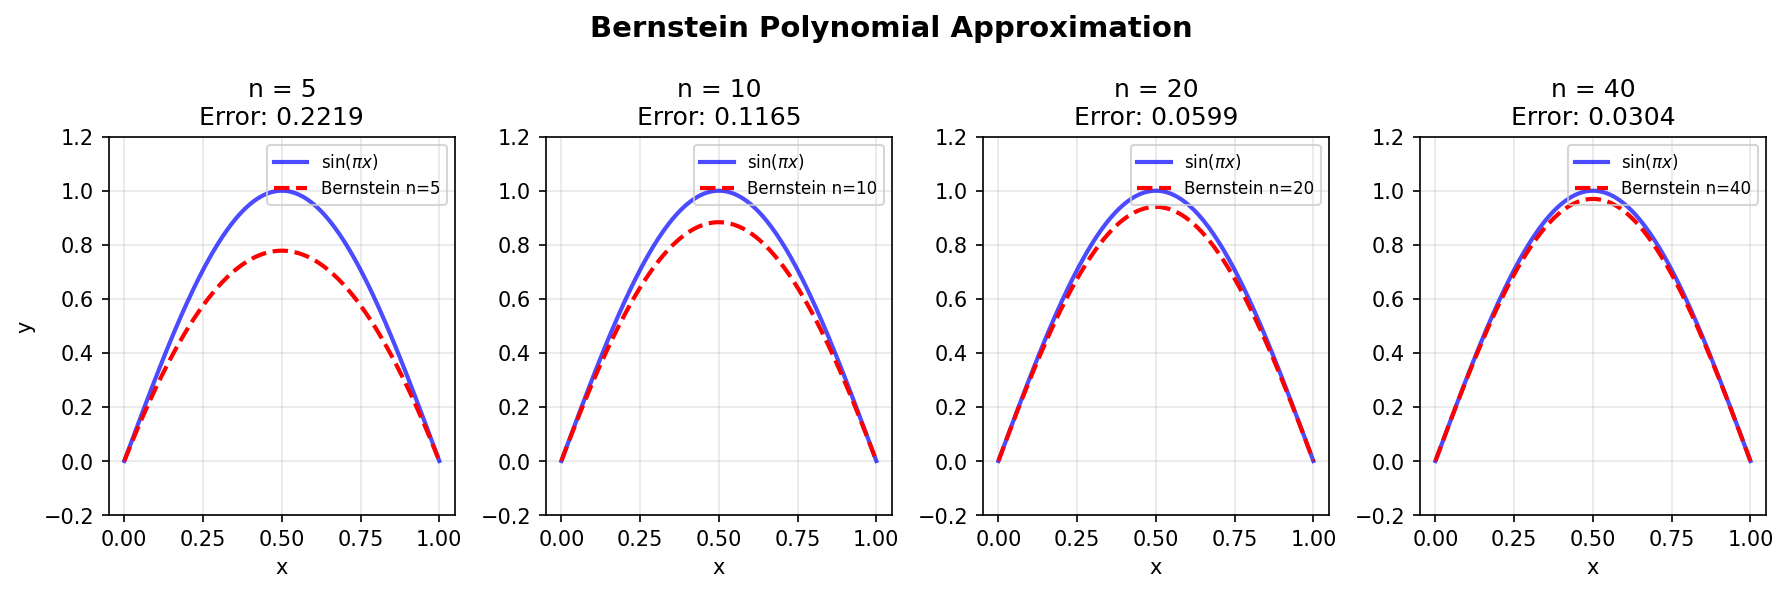
\includegraphics[width=0.62\textwidth]{figs/mlp-bernstein-approximation}}
\end{center}
\centering
\stepfrom{2}{\chip{Bernstein $B_n f$ for $\sin(\pi x)$, largest gap}{$0.222$, $0.117$, $0.060$, $0.030$ at $n = 5, 10, 20, 40$}}\quad
\chip{what the theorem does not say}{the degree, the weights, or the slopes}
\note{
The Weierstrass theorem guarantees a polynomial within any prescribed sup-norm tolerance of a continuous function on a closed interval.
It does not specify that polynomial or its degree.
Bernstein's formula provides one explicit sequence of such approximations.

The rate depends on the function's variation.
Its modulus of continuity is $\omega_f(\delta)=\sup_{|x-y|\le\delta}|f(x)-f(y)|$.
Continuity on the closed interval gives $\omega_f(\delta)\to0$ as $\delta\to0$, which is enough for convergence.
Continuity alone does not guarantee a $1/\sqrt n$ rate.

If $f$ is Lipschitz with constant $L$, then $|B_nf(x)-f(x)|\le L\,\mathbb{E}|X/n-x|\le L/(2\sqrt n)$.
The corner has this regularity and attains the $n^{-1/2}$ order.
If $f\in C^2[0,1]$, the zero mean of $X/n-x$ cancels the linear term.
The remaining error is bounded by $\|f''\|_\infty/(8n)$.

The sine example follows the faster $1/n$ rate.
Its sup errors are $0.222$, $0.117$, $0.060$, and $0.030$ at degrees $5$, $10$, $20$, and $40$.
Qualitative universal approximation theorems for networks similarly guarantee existence under their stated assumptions.
Their existence statement alone does not determine a useful network size or a training procedure.
}
\end{frame}

\begin{frame}{Convergence of Bernstein polynomials for a smooth function}
\begin{columns}
\column{0.7\textwidth}
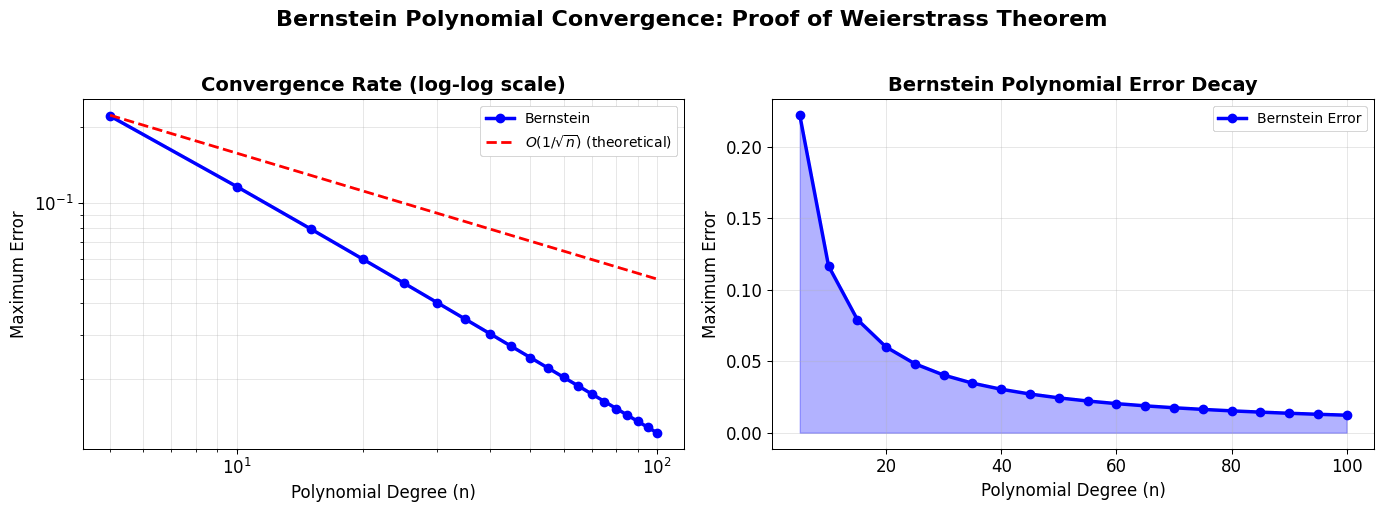
\includegraphics[width=\textwidth]{figs/mlp-polynomial-convergence}
\column{0.3\textwidth}
\chip{target}{$\sin(\pi x)$}\\[4pt]
\chip{largest gap, $n = 5$ and $n = 100$}{$0.22$ and $0.013$}\\[4pt]
\chip{Voronovskaya at mid-span, $\pi^2/(8n)$}{$0.25$ and $0.012$}
\end{columns}
\note{
For the corner, the Bernstein sup error decreases as $n^{-1/2}$.
For the smooth target $\sin(\pi x)$, it decreases as $n^{-1}$.
The measured error falls from $0.22$ at degree $5$ to $0.013$ at degree $100$.

Voronovskaya's formula gives $f-B_nf\approx-x(1-x)f''(x)/(2n)$.
At mid-span, its magnitude is $\pi^2/(8n)$, predicting $0.25$ and $0.012$ at these degrees.
The nonzero second derivative explains the leading $1/n$ error.
The dashed $n^{-1/2}$ comparison is a bound for Lipschitz targets, not for every merely continuous target.
Smoothness improves this example's rate, but Bernstein's construction remains much slower than the following least-squares fit.
}
\end{frame}

\begin{frame}{Least-squares polynomial approximation of $\sin(\pi x)$}
\begin{columns}
\column{0.62\textwidth}
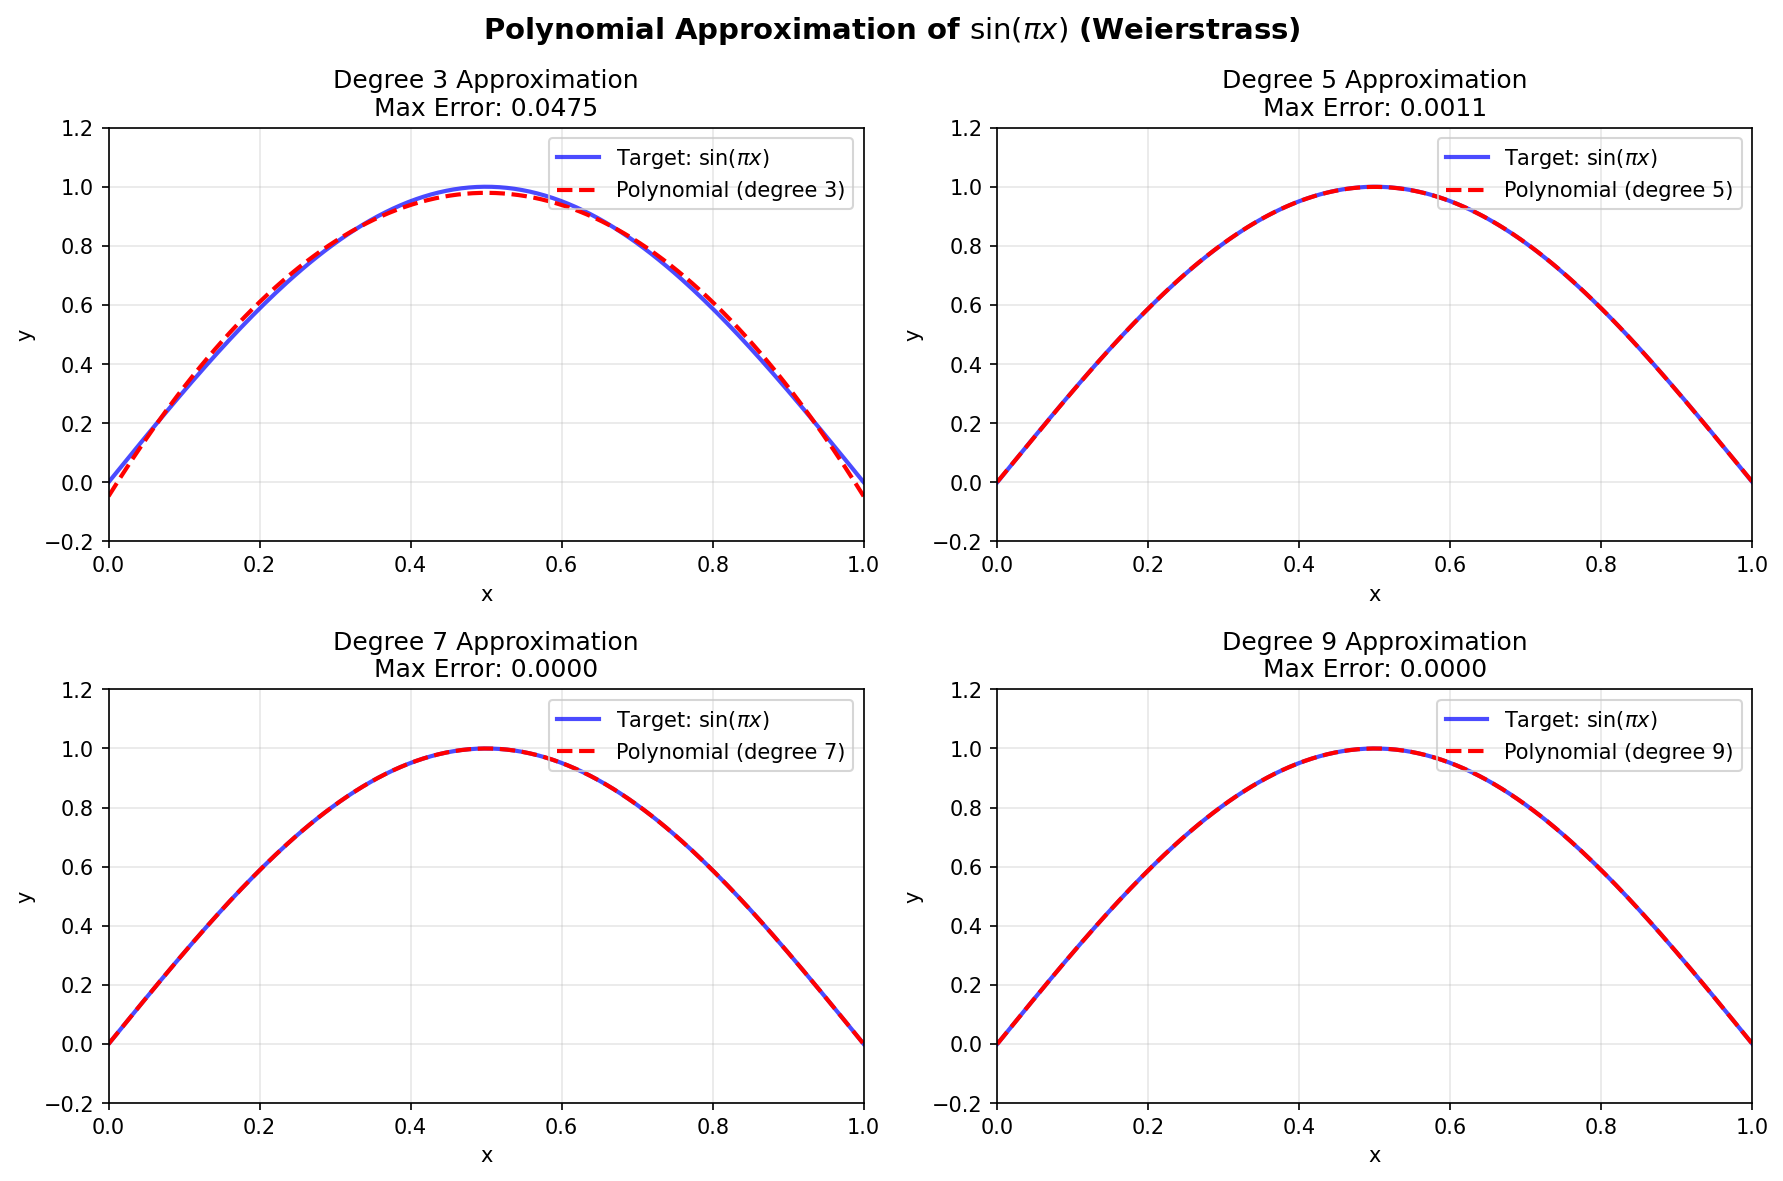
\includegraphics[width=\textwidth]{figs/mlp-polynomial-approximation-sinpi}
\column{0.38\textwidth}
\chip{degree $3$, largest gap}{$0.0475$}\\[4pt]
\chip{degree $5$, largest gap}{$0.0011$}\\[4pt]
\chip{degrees $7$ and $9$, largest gap}{below $0.00005$}
\end{columns}
\note{
The Bernstein construction does not minimize polynomial approximation error.
A least-squares fit to $\sin(\pi x)$ at one hundred points gives much smaller errors at low degree.
The measured sup errors are $0.0475$ at degree $3$, $0.0011$ at degree $5$, and below $0.00005$ at degrees $7$ and $9$.

The sine extends analytically beyond the interval, so its best polynomial errors decrease at least geometrically with degree.
Its Bernstein errors instead have a leading $1/n$ term.
The approximation family, the rule for selecting coefficients, and the convergence rate are separate choices.
}
\end{frame}

\begin{frame}{High-degree interpolation of noisy data}
\begin{columns}
\column{0.72\textwidth}
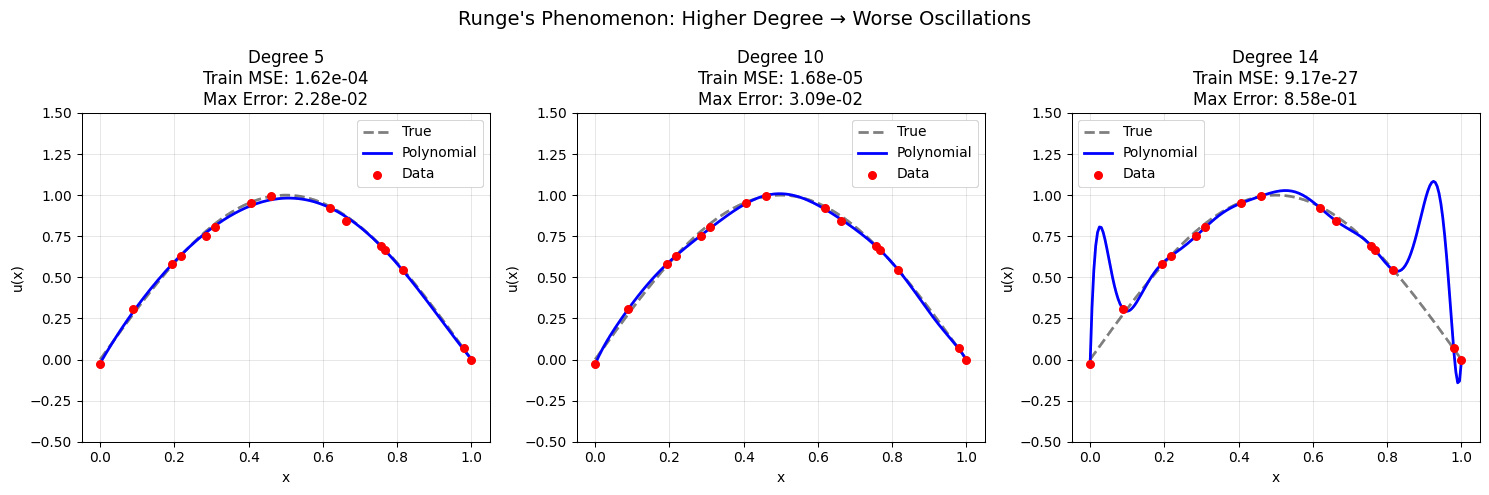
\includegraphics[width=\textwidth]{figs/mlp-polynomial-approx-sparse}
\column{0.28\textwidth}
\chip{degree $5$, least squares}{largest gap $0.023$}\\[4pt]
\chip{degree $10$, least squares}{largest gap $0.031$}\\[4pt]
\chip{degree $14$, through all fifteen noisy readings}{training mean squared error $9 \times 10^{-27}$, largest gap $0.86$}
\end{columns}
\note{
Now use fifteen scattered sine readings with Gaussian noise of standard deviation $0.02$.
Least-squares fits of degrees $5$ and $10$ have sup errors against the sine of $0.023$ and $0.031$.
The degree-$14$ interpolant reproduces every noisy reading with a root-mean-square residual near $10^{-13}$.
Its sup error against the sine is nevertheless $0.86$.

The interpolant oscillates strongly between readings near the ends.
Exact agreement with noisy measurements can therefore give poor recovery of the underlying function.
This experiment concerns noisy scattered data.
Runge's example instead concerns divergence of equispaced interpolation even for noiseless data.
}
\end{frame}

\begin{frame}{What the Weierstrass theorem does not say}

\medskip
\begin{columns}[T]
\column{0.5\textwidth}
\begin{tikzpicture}
\begin{axis}[rep, height=4.4cm, xmin=0.35, xmax=0.65, ymin=0, ymax=0.2, xlabel=$x$, legend pos=north east, title={\scriptsize $B_{32} f$ beside the corner}]
\addplot[ink, dashed, line width=1.2pt] table[x=x, y=f]{data/bern32.dat};
\addlegendentry{$|x - \tfrac12|$}
\addplot[sblue, line width=1.6pt] table[x=x, y=B]{data/bern32.dat};
\addlegendentry{$B_{32} f$, slope $0$ at $\tfrac12$}
\end{axis}
\end{tikzpicture}
\column{0.5\textwidth}
\chip{Bernstein sup error for this corner}{falls like $1/\sqrt{n}$}\\[4pt]
\chip{best degree-$n$ sup error for this corner}{falls like $1/n$}\\[4pt]
\chip{the theorem names}{no polynomial, no degree, no slope}
\end{columns}
\note{
The Weierstrass theorem concerns uniform error in function values.
It makes no claim about approximation of derivatives.
For the corner, the derivative is undefined at mid-span, although every Bernstein polynomial has a derivative there.

For this target, Bernstein's sup error decreases as $1/\sqrt n$ while the best degree-$n$ polynomial error decreases as $1/n$.
The existence theorem does not distinguish these rates.
It also does not guarantee a closest member among polynomials of all degrees.
Their error infimum is zero, but no polynomial equals the corner.

A fixed-degree polynomial space does have a unique $L^2$ projection.
Density over increasing degrees and optimality within one fixed space answer different questions.
Qualitative neural-network approximation theorems likewise require separate analysis of size, fitting, and stability.
}
\end{frame}

\begin{frame}{Polynomial density through vanishing moments}
\begin{columns}
\column{0.5\textwidth}
\small
\begin{tabular}{@{}rl@{}}
\toprule
moments forced to zero & response to $\sin(3\pi x)$ \\
\midrule
$0$ & $0.635$ \\
$2$ & $0.565$ \\
$4$ & $0.298$ \\
$8$ & $1.2 \times 10^{-3}$ \\
$16$ & $3.0 \times 10^{-9}$ \\
$32$ & $6.9 \times 10^{-16}$ \\
\bottomrule
\end{tabular}
\column{0.5\textwidth}
\small
\[
\int_0^1 x^k\,d\mu(x) = 0 \quad\text{for every } k
\]
\[
\Longrightarrow\quad \int_0^1 f\,d\mu = 0 \quad\text{for every continuous } f
\]
\chip{density criterion}{all polynomial moments zero implies the finite signed measure is zero}
\end{columns}
\note{
On a finite grid, a weighted sum of samples assigns a scalar to each function.
Adding or scaling functions adds or scales this scalar, so the weighted sum is a linear functional.
The table chooses weights whose sums against successive monomials are zero.
Their response to $\sin(3\pi x)$ decreases from $0.635$ to $1.2\times10^{-3}$ and then to numerical zero.

The continuum version is $L(f)=\int f\,d\mu$, where $\mu$ is a finite signed measure.
Its responses to monomials are the moments $\int x^k\,d\mu$.
It is bounded in the sup norm, meaning $|L(f)|\le C\|f\|_\infty$ for a fixed constant $C$.

If the polynomial span were not dense in $C[0,1]$, a separation theorem would give a bounded linear functional that vanishes on every polynomial but not on some continuous function.
The Riesz representation theorem writes it as an integral against such a measure.
Thus an independent proof that zero polynomial moments force $\mu=0$ proves density.
The displayed implication states this criterion.
The finite-grid table illustrates it but does not prove the infinite-dimensional result.
}
\end{frame}

\begin{frame}{Cauchy sequences, completeness, and Hilbert spaces}
\begin{columns}
\column{0.7\textwidth}
\begin{tikzpicture}
\begin{axis}[rep, height=6.2cm, xmin=0, xmax=1, ymin=-0.1, ymax=1.1, xlabel=$x$, legend pos=north west]
\addplot[ink, dashed, line width=1.2pt] coordinates {(0,0) (0.5,0) (0.5,1) (1,1)};
\addlegendentry{step}
\addplot[sblue!45, line width=1.4pt] table[x=x, y=r]{data/ramp2.dat};
\addlegendentry{$w = 1/2$}
\stepfrom{2}{\addplot[sblue!75, line width=1.4pt] table[x=x, y=r]{data/ramp8.dat};
          \addlegendentry{$w = 1/8$}}
\stepfrom{3}{\addplot[sblue, line width=1.4pt] table[x=x, y=r]{data/ramp32.dat};
          \addlegendentry{$w = 1/32$}}
\end{axis}
\end{tikzpicture}
\column{0.3\textwidth}
\chip{$L^2$ distance to the step, $\sqrt{w/12}$}{$0.204$ at $w = 1/2$}\\[4pt]
\stepfrom{2}{\chip{$w = 1/8$}{$0.102$}\\[4pt]}
\stepfrom{3}{\chip{$w = 1/32$}{$0.051$}\\[4pt]
\chip{$\|f_8 - f_{32}\|_{L^2}$}{$0.077$}}
\end{columns}
\note{
A continuous ramp of width $w$ has $L^2$ distance $\sqrt{w/12}$ from the step.
As $w$ tends to zero, this distance tends to zero.
The triangle inequality also bounds the distance between two ramps by the sum of their distances to the step.

The narrowing ramps therefore form a Cauchy sequence in $L^2$.
Every ramp is continuous, but the limit is discontinuous.
The continuous functions are incomplete under this norm.
Their completion is $L^2$, where every Cauchy sequence has a limit.
With its inner product, this complete space is a Hilbert space.
}
\end{frame}

\begin{frame}{Point evaluation in $L^2$ and $H^1$}
\begin{columns}
\column{0.6\textwidth}
\begin{tikzpicture}
\begin{axis}[rep, height=6cm, xmin=0, xmax=1, ymin=-1.5, ymax=1.6, xlabel=$x$, ylabel=$u(x)$, legend pos=south west]
\addplot[ink, line width=1.4pt] table[x=x, y=u]{data/string.dat};
\addlegendentry{the displacement}
\addplot[only marks, mark=o, mark size=2.6pt, sred, line width=1pt] coordinates {(0.6, 0.408)};
\addplot[only marks, mark=*, mark size=2.6pt, sred] coordinates {(0.6, 0.908)};
\addlegendentry{the same function with $u(0.6)$ moved by $0.5$}
\stepfrom{2}{\addplot[sblue, line width=1.2pt] coordinates {(0.6, 0.408) (0.8, 0.408)};
          \addplot[sblue, line width=1.2pt, dashed] coordinates {(0.8, 0.408) (0.8, 0.28)};
          \node[font=\tiny, sblue, anchor=south west] at (axis cs:0.81, 0.30) {$\le \sqrt{0.2}\,|u|_{H^1}$};}
\end{axis}
\end{tikzpicture}
\column{0.4\textwidth}
\chip{$L^2$ distance between the two}{$0$}\\[6pt]
\stepfrom{2}{\[
|u(y) - u(x)| = \Bigl|\int_x^y u'(s)\,ds\Bigr| \le \sqrt{y - x}\; |u|_{H^1}
\]}
\end{columns}
\note{
The plotted functions differ only at $x=0.6$, where one value is $0.5$ higher.
Their $L^2$ distance is zero.
They represent the same $L^2$ element, so that element does not determine a unique point value.

For $u\in H^1(0,1)$, the weak derivative controls differences between values of its continuous representative.
The integral identity and Cauchy-Schwarz inequality give $|u(y)-u(x)|\le\sqrt{|y-x|}\,\|u'\|_{L^2}$.
This representative is unique, so point readings are well defined on the interval.
The finite-energy string belongs to this space.

The cooling fin gives a different reconstruction problem.
Its temperature is unknown, and only noisy readings are available.
Which assumptions permit a temperature estimate between the sensors?
}
\end{frame}

%========================================================================================
\repsection{Kernels}{Kernels and point evaluation}

\begin{frame}{Linear regression by least squares}
\begin{columns}
\column{0.6\textwidth}
\begin{tikzpicture}
\begin{axis}[rep, height=5.8cm, xmin=-3.5, xmax=3.5, ymin=-1.6, ymax=1.6, xlabel=$x$, ylabel=$y$, legend pos=north west]
\addplot[muted, dashed, line width=1pt] table[x=x, y=s]{data/reg_fits.dat};
\addlegendentry{$\sin x$, unknown to the fit}
\addplot[only marks, mark=*, mark size=2.2pt, sred] table[x=x, y=y]{data/reg_data.dat};
\addlegendentry{twelve noisy readings}
\stepfrom{2}{\addplot[sblue, line width=1.6pt] table[x=x, y=line]{data/reg_fits.dat};
          \addlegendentry{line, features $1, x$}}
\stepfrom{3}{\addplot[sgreen, line width=1.6pt] table[x=x, y=cubic]{data/reg_fits.dat};
          \addlegendentry{cubic, features $1, x, x^2, x^3$}}
\end{axis}
\end{tikzpicture}
\column{0.4\textwidth}
\small
\[
\hat y(x) = \sum_{j} w_j\,\phi_j(x), \qquad \min_{\mathbf{w}} \|\boldsymbol{\Phi}\mathbf{w} - \mathbf{y}\|^2
\]
\[
\boldsymbol{\Phi}^\top\boldsymbol{\Phi}\,\mathbf{w} = \boldsymbol{\Phi}^\top\mathbf{y}
\]
\stepfrom{2}{\chip{line, RMSE at the data and against $\sin x$}{$0.484$ and $0.439$}\\[4pt]}
\stepfrom{3}{\chip{cubic, the same two errors}{$0.119$ and $0.085$}}
\end{columns}
\note{
The regression example uses twelve readings $y_i=\sin x_i+\varepsilon_i$ on $[-3,3]$.
The noise has standard deviation $0.15$.
A fit $\hat f=\sum_j w_j\phi_j$ chooses coefficients to minimize squared disagreement at these readings.

Writing $\Phi_{ij}=\phi_j(x_i)$ gives the normal equations $\boldsymbol{\Phi}^{\top}\boldsymbol{\Phi}\mathbf{w}=\boldsymbol{\Phi}^{\top}\mathbf{y}$.
The sampled residual is orthogonal to the columns of $\boldsymbol{\Phi}$ in the Euclidean data inner product.
This is a projection of the measurement vector, rather than an $L^2$ projection of the unknown function.

The line has RMSE $0.484$ at the readings and $0.439$ against the reference sine.
The cubic reduces these errors to $0.119$ and $0.085$.
Adding features can reduce training error, but it need not improve recovery between readings.
What happens when the number of coefficients equals the number of measurements?
}
\end{frame}

\begin{frame}{Ridge regression on many features}
\begin{columns}
\column{0.6\textwidth}
\begin{tikzpicture}
\begin{axis}[rep, height=5.8cm, xmin=-3.5, xmax=3.5, ymin=-2.5, ymax=2.5, xlabel=$x$, ylabel=$y$, legend pos=north west]
\addplot[muted, dashed, line width=1pt] table[x=x, y=s]{data/reg_fits.dat};
\addlegendentry{$\sin x$}
\addplot[only marks, mark=*, mark size=2.2pt, sred] table[x=x, y=y]{data/reg_data.dat};
\addlegendentry{readings}
\steponly{1}{2}{\addplot[sorange, line width=1.6pt] table[x=x, y=deg11]{data/reg_fits.dat};
          \addlegendentry{degree $11$, least squares}}
\steponly{2}{2}{\addplot[sorange!45, line width=1.2pt, forget plot] table[x=x, y=deg11]{data/reg_fits.dat};
          \addplot[sblue, line width=1.6pt] table[x=x, y=deg11ridge]{data/reg_fits.dat};
          \addlegendentry{degree $11$, ridge $\lambda = 10^{-3}$}}
\end{axis}
\end{tikzpicture}
\column{0.4\textwidth}
\small
\[
\min_{\mathbf{w}} \|\boldsymbol{\Phi}\mathbf{w} - \mathbf{y}\|^2 + \lambda\|\mathbf{w}\|^2
\]
\[
(\boldsymbol{\Phi}^\top\boldsymbol{\Phi} + \lambda\mathbf{I})\,\mathbf{w} = \boldsymbol{\Phi}^\top\mathbf{y}
\]
\chip{degree $11$, least squares}{error at the data $0$, largest weight $284$, swings to $29.5$}\\[4pt]
\stepfrom{2}{\chip{degree $11$, ridge}{error against $\sin x$ $0.073$, largest weight $4.3$}}
\end{columns}
\note{
Use the twelve features $1,x/3,\ldots,(x/3)^{11}$.
Their least-squares fit interpolates all twelve readings.
The largest coefficient is $284$, and the curve reaches $29.5$ outside the last sensor locations.
Agreement with the noisy readings gives no guarantee of an accurate profile.

Ridge regression adds the coefficient penalty $\lambda\|\mathbf{w}\|^2$.
Its normal equations are $(\boldsymbol{\Phi}^{\top}\boldsymbol{\Phi}+\lambda\mathbf{I})\mathbf{w}=\boldsymbol{\Phi}^{\top}\mathbf{y}$.
The positive diagonal term reduces amplification associated with small eigenvalues.

At $\lambda=10^{-3}$, the largest coefficient falls to $4.3$.
The RMSE against the sine falls to $0.073$.
This penalty depends on the chosen feature scaling.
Can an inner product specify the features and their penalty without listing every feature?
}
\end{frame}

\begin{frame}{A kernel is an inner product of features}
\begin{columns}
\column{0.58\textwidth}
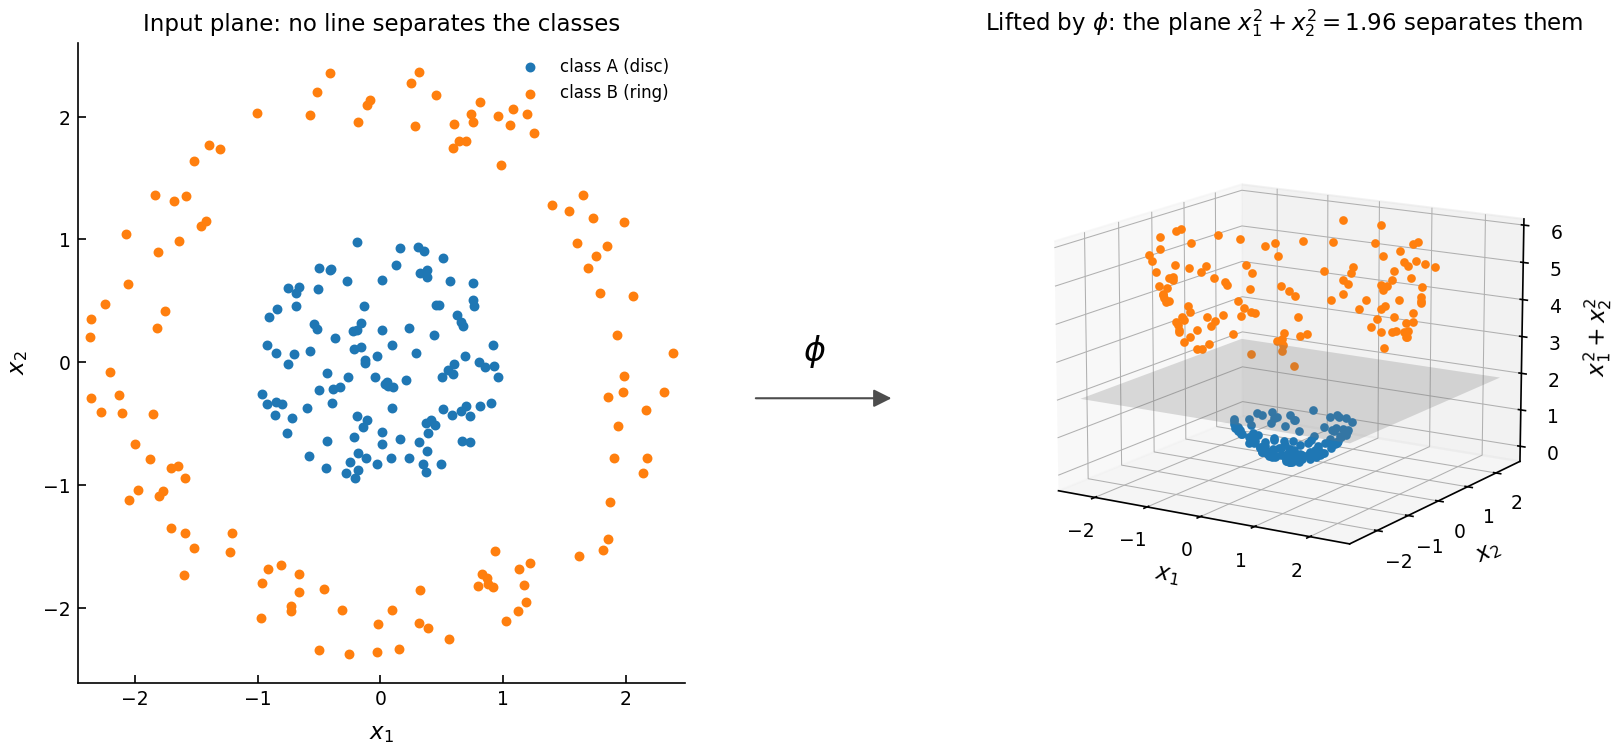
\includegraphics[width=\textwidth]{figs/ka-feature-map}
\column{0.42\textwidth}
\small
\[
\phi(x_1, x_2) = (x_1,\ x_2,\ x_1^2 + x_2^2)
\]
\[
k(\mathbf{x}, \mathbf{x}') = \phi(\mathbf{x})\cdot\phi(\mathbf{x}') = \mathbf{x}\cdot\mathbf{x}' + |\mathbf{x}|^2|\mathbf{x}'|^2
\]
\chip{a plane in feature space}{$x_3 = 1.96$ separates disc from ring, no errors}\\[4pt]
\chip{$\mathbf{x} = (1, 0)$, $\mathbf{x}' = (0.5, 0.5)$}{both routes give $1.000$}
\end{columns}
\note{
A disc and a surrounding ring cannot be separated by a line in the original plane.
The feature map $\phi(x_1,x_2)=(x_1,x_2,x_1^2+x_2^2)$ adds squared radius as a coordinate.
The plane $x_3=1.96$ separates the plotted feature vectors without classification errors.

For these features, $\phi(\mathbf{x})\cdot\phi(\mathbf{x}')=\mathbf{x}\cdot\mathbf{x}'+|\mathbf{x}|^2|\mathbf{x}'|^2$.
The inner product can therefore be computed directly from the original coordinates.
Both calculations give $1.000$ for the displayed pair.
A kernel is a function $k(\mathbf{x},\mathbf{x}')$ that supplies such feature inner products.

The Gram matrix $K_{ij}=k(\mathbf{x}_i,\mathbf{x}_j)$ is positive semidefinite because it is a matrix of inner products.
Methods written in terms of these inner products can use $k$ without constructing the feature vectors.
The Gaussian kernel corresponds to an infinite-dimensional feature map.
A general linear computation need not depend only on feature inner products.
}
\end{frame}

\begin{frame}{Regression on Gaussian bump features}
\begin{columns}
\column{0.62\textwidth}
\begin{tikzpicture}
\begin{axis}[rep, height=5.8cm, xmin=-3.1, xmax=3.1, ymin=-2, ymax=2, xlabel=$x$, legend pos=north west]
\addplot[muted, line width=1.6pt] table[x=x, y=f]{data/bumps_m5.dat};
\addlegendentry{target $\sin(1.5x) + 0.5\sin(4x)$}
\steponly{1}{2}{\addplot[sblue, dashed, line width=1pt, forget plot] table[x=x, y=b0]{data/bumps_m5.dat};
\addplot[sorange, dashed, line width=1pt, forget plot] table[x=x, y=b1]{data/bumps_m5.dat};
\addplot[sgreen, dashed, line width=1pt, forget plot] table[x=x, y=b2]{data/bumps_m5.dat};
\addplot[sred, dashed, line width=1pt, forget plot] table[x=x, y=b3]{data/bumps_m5.dat};
\addplot[violet, dashed, line width=1pt, forget plot] table[x=x, y=b4]{data/bumps_m5.dat};
          \addplot[sblue, line width=2pt] table[x=x, y=sum]{data/bumps_m5.dat};
          \addlegendentry{sum of $5$ bumps, $\ell = 0.5$}
          \addplot[only marks, mark=*, mark size=2pt, ink, forget plot] table[x=x, y=y]{data/bumps_m5_centers.dat};}
\steponly{2}{2}{\foreach \j in {0,...,19} {\addplot[muted, dashed, line width=0.6pt, forget plot] table[x=x, y=b\j]{data/bumps_m20.dat};}
          \addplot[sblue, line width=2pt] table[x=x, y=sum]{data/bumps_m20.dat};
          \addlegendentry{sum of $20$ bumps, $\ell = 0.5$}
          \addplot[only marks, mark=*, mark size=1.5pt, ink, forget plot] table[x=x, y=y]{data/bumps_m20_centers.dat};}
\end{axis}
\end{tikzpicture}
\column{0.38\textwidth}
\small
\[
\hat f(x) = \sum_{j=1}^{m} w_j\, e^{-(x - c_j)^2/2\ell^2}
\]
\chip{$5$ bumps, $\ell = 0.5$}{RMSE $0.442$}\\[4pt]
\stepfrom{2}{\chip{$20$ bumps, $\ell = 0.5$}{RMSE $0.002$}\\[4pt]
\chip{$20$ bumps, narrow $\ell = 0.1$ and wide $\ell = 2$}{$0.191$ with gaps, $0.316$ blurred}}
\end{columns}
\note{
Place Gaussian bump features at $m$ equally spaced centers on $[-3,3]$.
Fit their amplitudes to $\sin(1.5x)+0.5\sin(4x)$.
The least-squares objective includes a fixed small ridge penalty to stabilize the solve.

Five bumps of width $0.5$ give RMSE $0.442$.
Twenty bumps of the same width reduce it to $0.002$.
At twenty bumps, width $0.1$ gives RMSE $0.191$, while width $2$ gives $0.316$.

The narrow bumps leave poorly represented intervals between centers.
The wide bumps are strongly correlated, and the fixed penalty suppresses the coefficients needed for the rapid variation.
These errors depend on the spacing, width, target, and penalty together.
The companion kernel-approximation notebook varies these choices.
}
\end{frame}

\begin{frame}{Kernel ridge regression with copies at the data}
\begin{columns}
\column{0.6\textwidth}
\begin{tikzpicture}
\begin{axis}[rep, height=5.8cm, xmin=-4, xmax=4, ymin=-1.6, ymax=1.6, xlabel=$x$, legend pos=north west]
\addplot[muted, dashed, line width=1pt] table[x=x, y=s]{data/krr_copies.dat};
\addlegendentry{$\sin x$}
\stepfrom{2}{\foreach \i in {0,...,11} {\addplot[gray, dashed, line width=0.7pt, forget plot] table[x=x, y=c\i]{data/krr_copies.dat};}}
\stepfrom{3}{\addplot[ink, line width=2pt] table[x=x, y=sum]{data/krr_copies.dat};
          \addlegendentry{$\sum_i \alpha_i k(x, x_i)$}}
\addplot[only marks, mark=*, mark size=2.2pt, sred] table[x=x, y=y]{data/reg_data.dat};
\addlegendentry{twelve readings}
\end{axis}
\end{tikzpicture}
\column{0.4\textwidth}
\small
\[
\hat f(x) = \sum_{i=1}^{12} \alpha_i\, k(x, x_i), \qquad (\mathbf{K} + \lambda\mathbf{I})\,\boldsymbol{\alpha} = \mathbf{y}
\]
\stepfrom{2}{\chip{weights, $\ell = 1/\sqrt3$, $\lambda = 0.01$}{from $-0.632$ to $1.129$}\\[4pt]}
\stepfrom{3}{\chip{RMSE at the readings and against $\sin x$}{$0.0051$ and $0.113$}}
\end{columns}
\note{
Place a kernel copy at each reading and write $\hat f(x)=\sum_i\alpha_i k(x,x_i)$.
Kernel ridge regression minimizes $\sum_i(f(x_i)-y_i)^2+\lambda\|f\|_k^2$ over the kernel's Hilbert space.
The representer theorem gives a minimizer in the span of these copies.

For this expansion, the data term is $\|\mathbf{K}\boldsymbol{\alpha}-\mathbf{y}\|^2$ and the squared RKHS norm is $\boldsymbol{\alpha}^{\top}\mathbf{K}\boldsymbol{\alpha}$.
The coefficients satisfy $(\mathbf{K}+\lambda\mathbf{I})\boldsymbol{\alpha}=\mathbf{y}$.
This is not ordinary ridge regression with a penalty $\|\boldsymbol{\alpha}\|^2$.

At $\ell=1/\sqrt3$ and $\lambda=0.01$, the weights range from $-0.632$ to $1.129$.
The sum has RMSE $0.0051$ against the readings and $0.113$ against the reference sine at those locations.
The much smaller training residual indicates that the fitted function reproduces part of the measurement noise.
For the cooling fin, the same reconstruction must be assessed without knowing the reference profile.
}
\end{frame}


\begin{frame}{Kernels as similarity rules for scattered readings}
\begin{columns}
\column{0.7\textwidth}
\begin{tikzpicture}
\begin{axis}[rep, height=6.2cm, xmin=0, xmax=1, ymin=-0.3, ymax=1.3, xlabel=$x$, ylabel=$T(x)$, legend pos=north east]
\addplot[only marks, mark=*, mark size=2.4pt, sred] table[x=x, y=y]{data/fin_readings.dat};
\addlegendentry{eight readings}
\stepfrom{2}{\addplot[ink, dashed, line width=1.2pt] table[x=x, y=T]{data/fin_true.dat};
          \addlegendentry{true profile, unknown in practice}}
\stepfrom{3}{\addplot[sblue, line width=1.4pt] table[x=x, y=k1]{data/kernel_pair.dat};
          \addlegendentry{copy at $0.30$, $\ell = 0.15$}
          \addplot[sorange, line width=1.4pt] table[x=x, y=k2]{data/kernel_pair.dat};
          \addlegendentry{copy at $0.45$}}
\end{axis}
\end{tikzpicture}
\column{0.3\textwidth}
\stepfrom{3}{\[
k(x, x') = e^{-(x - x')^2/2\ell^2}
\]
\chip{$k(0.30, 0.45)$, one $\ell$ apart}{$0.61$}\\[4pt]
\chip{$k$ at $3\ell$ apart}{$0.011$}}
\end{columns}
\note{
For the cooling fin, the temperature profile is unknown.
The readings $y_i$ constrain it at locations $x_i\in[0,1]$, where $x$ is normalized distance along the fin.
Infinitely many curves agree with these readings.
How should a measurement affect the estimate at a neighboring location?

Heat conduction motivates a smooth profile.
The squared-exponential kernel $k(x,x')=\exp(-(x-x')^2/(2\ell^2))$ assigns greater similarity to nearby locations.
The length scale $\ell$ sets the spatial decay of that similarity.
Its suitability must be checked against the measurements.

Copies centered at $0.30$ and $0.45$ are one length scale apart and have kernel value $0.61$.
At separation $3\ell$, the value falls to $0.011$.
A weighted sum of the copies defines the estimate $\hat f(x)=\sum_i\alpha_i k(x,x_i)$.
Because the copies overlap, their coefficients must be chosen together.
}
\end{frame}

\begin{frame}{Reconstructing a profile with weighted kernel copies}
\begin{columns}
\column{0.7\textwidth}
\begin{tikzpicture}
\begin{axis}[rep, height=6.2cm, xmin=0, xmax=1, ymin=-4, ymax=4.5, xlabel=$x$, legend pos=north east]
\addplot[only marks, mark=*, mark size=2.4pt, sred] table[x=x, y=y]{data/fin_readings.dat};
\foreach \i in {0,...,7} {\addplot[muted, dashed, line width=0.8pt] table[x=x, y=b\i]{data/bumps15.dat};}
\addplot[sblue, line width=1.8pt] table[x=x, y=sum]{data/bumps15.dat};
\addlegendentry{sum of the weighted copies, $\ell = 0.15$}
\stepfrom{2}{\addplot[sorange, line width=1.8pt] table[x=x, y=sum]{data/bumps04.dat};
         \addlegendentry{sum, $\ell = 0.04$}
         \addplot[ink, dashed, line width=1pt] table[x=x, y=T]{data/fin_true.dat};
         \addlegendentry{true profile}}
\end{axis}
\end{tikzpicture}
\column{0.3\textwidth}
\[
\mathbf{K}\boldsymbol{\alpha} = \mathbf{y}, \qquad K_{ij} = k(x_i, x_j)
\]
\chip{weights at $\ell = 0.15$}{alternate in sign, up to $4.30$ and $-3.75$}\\[4pt]
\chip{two equal readings one $\ell$ apart}{$1/(1+\rho) = 0.62$ each}\\[4pt]
\chip{at $x = 0.7$, $\ell = 0.15$}{$0.216$ against the reference $0.393$}\\[4pt]
\stepfrom{2}{\chip{sum at $x = 0.7$, $\ell = 0.04$}{$0.000$ against the true $0.393$}}
\end{columns}
\note{
Requiring $\hat f(x_i)=y_i$ gives the interpolation system $\mathbf{K}\boldsymbol{\alpha}=\mathbf{y}$.
For distinct sites, the squared-exponential kernel gives a symmetric positive-definite matrix.
The coefficients are unique, but this guarantees only agreement at the sensors.

For two sensors separated by $\ell$ with readings one, symmetry gives equal coefficients.
At either site, $\alpha+\rho\alpha=1$, where $\rho=e^{-1/2}$.
Thus each coefficient is $1/(1+\rho)=0.62$.
A coefficient differs from its reading because the neighboring copy also contributes.

The synthetic fin has a reference profile for checking the reconstruction.
At $\ell=0.15$, the coefficients include $4.30$ and $-3.75$.
The reconstructed value at $x=0.7$ is $0.216$, compared with the reference $0.393$.
At $\ell=0.04$, it is below $0.001$, although every reading is still interpolated.
Sensor agreement alone does not validate a length scale.
}
\end{frame}

\begin{frame}{Positive definiteness of a kernel}
\begin{columns}
\column{0.5\textwidth}
\begin{center}
\begin{tikzpicture}[font=\small]
\draw[ink, thick] (0,0) -- (6,0);
\foreach \x/\l in {0.5/$0$, 2.9/$0.6\ell$, 5.3/$1.2\ell$} {\fill[sblue] (\x,0) circle (3pt); \node[below] at (\x,-0.1) {\l};}
\draw[sgreen, thick] (0.5,0.35) to[bend left=35] node[above, font=\scriptsize] {similar, $1$} (2.9,0.35);
\draw[sgreen, thick] (2.9,0.35) to[bend left=35] node[above, font=\scriptsize] {similar, $1$} (5.3,0.35);
\draw[sred, thick, dashed] (0.5,-0.7) to[bend right=25] node[below, font=\scriptsize] {unrelated, $0$} (5.3,-0.7);
\end{tikzpicture}
\end{center}
\[
\mathbf{K} = \begin{pmatrix} 1 & 1 & 0 \\ 1 & 1 & 1 \\ 0 & 1 & 1 \end{pmatrix}, \qquad \lambda = 1 - \sqrt2,\ 1,\ 1 + \sqrt2
\]
\column{0.5\textwidth}
\[
\mathbf{w} = (1, -\sqrt2, 1), \qquad \mathbf{w}^\top\mathbf{K}\mathbf{w} = -1.66
\]
\medskip
\[
k(x, x') = \phi(x)^\top\phi(x') \;\Rightarrow\; \mathbf{w}^\top\mathbf{K}\mathbf{w} = \Bigl\|\sum_i w_i\,\phi(x_i)\Bigr\|^2 \ge 0
\]
\end{columns}
\note{
Consider a proposed kernel equal to one at separations below $\ell$ and zero otherwise.
At sites $0$, $0.6\ell$, and $1.2\ell$, it gives the displayed matrix.
The vector $(1,-\sqrt2,1)$ gives quadratic form $4-4\sqrt2=-1.66$.
Such a matrix cannot represent inner products because a squared norm cannot be negative.

A symmetric positive-definite kernel requires nonnegative quadratic forms for every finite collection of sites and weights.
This terminology permits positive-semidefinite Gram matrices.
Strict positive definiteness requires a positive value for nonzero weights at distinct sites.
The squared-exponential kernel has this stronger property.

Feature inner products give $\mathbf{w}^{\top}\mathbf{K}\mathbf{w}=\|\sum_i w_i\Phi(x_i)\|^2\ge0$.
Conversely, every positive-definite kernel admits a feature representation in a Hilbert space.
The features may be infinite-dimensional.
What geometry does this kernel give the reconstructed functions?
}
\end{frame}

\begin{frame}{The reproducing kernel Hilbert space}
\begin{columns}
\column{0.6\textwidth}
\begin{tikzpicture}
\begin{axis}[rep, height=6.2cm, xmin=0, xmax=1, ymin=-0.6, ymax=1.2, xlabel=$x$, legend pos=north west]
\addplot[sblue, dashed, line width=1.1pt] table[x=x, y=c0]{data/rkhs.dat};
\addlegendentry{$0.8\,k(0.2, \cdot)$}
\addplot[sorange, dashed, line width=1.1pt] table[x=x, y=c1]{data/rkhs.dat};
\addlegendentry{$-0.45\,k(0.5, \cdot)$}
\addplot[sgreen, dashed, line width=1.1pt] table[x=x, y=c2]{data/rkhs.dat};
\addlegendentry{$0.65\,k(0.8, \cdot)$}
\stepfrom{2}{\addplot[ink, line width=1.8pt] table[x=x, y=f]{data/rkhs.dat};
          \addlegendentry{$f$, their sum}}
\stepfrom{3}{\addplot[sred, dotted, line width=1.1pt] table[x=x, y=kp]{data/rkhs.dat};
          \addplot[sred, dashed, line width=0.8pt] coordinates {(0.72, -0.6) (0.72, 1.2)};
          \addplot[only marks, mark=*, mark size=2.6pt, sred] coordinates {(0.72, 0.403)};
          \node[font=\scriptsize, sred, anchor=south east] at (axis cs:0.99, -0.58) {$f(x^*) = 0.403$};}
\end{axis}
\end{tikzpicture}
\column{0.4\textwidth}
\[
\langle k(x_1, \cdot), k(x_2, \cdot)\rangle_k = k(x_1, x_2)
\]
\stepfrom{2}{\chip{$\|f\|_k^2 = \boldsymbol{\alpha}^\top\mathbf{K}\boldsymbol{\alpha}$, $\ell = 0.16$}{$1.041$}\\[4pt]}
\stepfrom{3}{\[
f(x) = \langle f, k(x, \cdot)\rangle_k
\]
\chip{$f(0.72)$, read as an inner product}{$0.403$, bound $1.02$}\\[4pt]
\chip{slope bound}{$|f'(x)| \le \|f\|_k/\ell$}}
\end{columns}
\note{
A squared-exponential copy has squared kernel norm $k(x_i,x_i)=1$.
Two copies have kernel inner product $\rho=k(x_1,x_2)$.
Their sum has squared norm $2+2\rho$, and their difference has squared norm $2-2\rho$.
Nearby copies are therefore close in this norm.

Linearity defines the inner product of finite weighted sums.
Completing these sums gives the reproducing kernel Hilbert space $\mathcal{H}_k$.
Its defining identity is $\langle k(x_1,\cdot),k(x_2,\cdot)\rangle_k=k(x_1,x_2)$.
This inner product is generally different from integrating the product of the two copies.

Taking the inner product of a weighted sum with $k(x,\cdot)$ evaluates that sum at $x$.
The identity extends to every member as $f(x)=\langle f,k(x,\cdot)\rangle_k$.
For the illustrated function, $\|f\|_k^2=1.041$ and $f(0.72)=0.403$.
Cauchy-Schwarz gives $|f(x)|\le\|f\|_k\sqrt{k(x,x)}$, with bound $1.02$ here.

For this kernel, derivative evaluation also gives $|f'(x)|\le\|f\|_k/\ell$.
Increasing by one across distance $\ell/10$ requires a slope of at least $10/\ell$ somewhere.
Such a function must have RKHS norm at least ten.
The norm therefore controls both amplitude and variation.
}
\end{frame}

%========================================================================================
\repsection{Noise}{Noisy observations, ridge regression, and Gaussian conditioning}

\begin{frame}{Noise amplification in kernel interpolation}
\begin{columns}
\column{0.6\textwidth}
\begin{tikzpicture}
\begin{axis}[rep, height=5.6cm, xmin=0, xmax=1, ymin=-0.2, ymax=1.3, xlabel=$x$, legend pos=north east]
\addplot[sblue, line width=1.3pt, domain=0:1, samples=201] {exp(-(x-0.4894)^2/(2*0.15^2))};
\addplot[sorange, line width=1.3pt, domain=0:1, samples=201] {exp(-(x-0.5106)^2/(2*0.15^2))};
\addlegendentry{two copies, overlap $0.99$}
\stepfrom{2}{\addplot[sred, line width=1.6pt, domain=0:1, samples=201] {7*(exp(-(x-0.4894)^2/(2*0.15^2)) - exp(-(x-0.5106)^2/(2*0.15^2)))};
          \addlegendentry{$7(\phi_1 - \phi_2)$}}
\end{axis}
\end{tikzpicture}
\column{0.4\textwidth}
\chip{eigenvalues of $\mathbf{K}$, overlap $0.99$}{$1.99$ along $(1,1)$, $0.01$ along $(1,-1)$}\\[4pt]
\chip{readings $(1, 1)$}{weights near $\tfrac12$ each}\\[4pt]
\stepfrom{2}{\chip{noise $(\varepsilon, -\varepsilon)$}{weights $\pm\varepsilon/0.01$, a hundred times the noise}\\[4pt]
\chip{RKHS norm of the perturbation}{$14.1|\varepsilon|$, distinct from pointwise error}}
\end{columns}
\note{
For two nearby sensors with similarity $\rho=0.99$, the kernel matrix has eigenvalues $1.99$ and $0.01$.
Equal changes in the readings use the first eigenvalue.
Opposite changes use the small eigenvalue and are strongly amplified.

Measurement errors $(\varepsilon,-\varepsilon)$ change the interpolation coefficients by $(100\varepsilon,-100\varepsilon)$.
The reconstructed perturbation is $100\varepsilon(\phi_1-\phi_2)$.
Its RKHS norm is about $14.1|\varepsilon|$ because $\|\phi_1-\phi_2\|_k=\sqrt{2-2\rho}$.
This is a function-norm change, not a pointwise error of fourteen times the noise.
}
\end{frame}

\begin{frame}{Kernel ridge regression and the choice of $\lambda$}
\begin{columns}
\column{0.5\textwidth}
\[
\min_{f \in \mathcal{H}_k} \sum_{i=1}^{n} \bigl(f(x_i) - y_i\bigr)^2 + \lambda \|f\|_k^2
\]
\[
(\mathbf{K} + \lambda\mathbf{I})\boldsymbol{\alpha} = \mathbf{y}
\]
\medskip
\centering
\chip{$\lambda = 0.1$, small divisor}{$0.01 \to 0.11$}\quad\chip{amplification}{$100$ to $9.1$}
\column{0.5\textwidth}
\begin{figure}
\centering
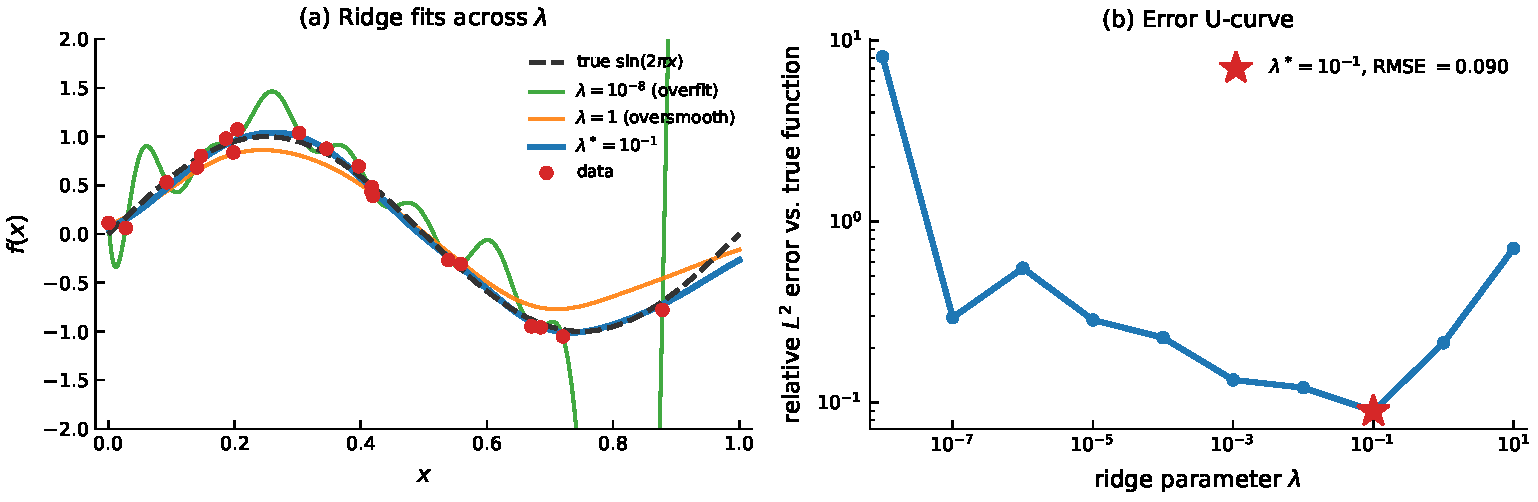
\includegraphics[width=0.8\textwidth]{figs/ridge-ucurve}
\end{figure}
\end{columns}
\note{
Kernel ridge regression permits disagreement with noisy readings and penalizes the RKHS norm.
Its objective is $\sum_i(f(x_i)-y_i)^2+\lambda\|f\|_k^2$ for $\lambda>0$.
The parameter $\lambda$ balances sensor fit against the amplitude and variation measured by the kernel norm.

A component orthogonal to the sensor copies has zero value at every sensor.
Removing that component leaves the data term unchanged and reduces the squared norm.
The minimizer therefore lies in the span of the copies and satisfies $(\mathbf{K}+\lambda\mathbf{I})\boldsymbol{\alpha}=\mathbf{y}$.

In the two-sensor example, $\lambda=0.1$ increases the small divisor from $0.01$ to $0.11$.
The corresponding coefficient amplification decreases from $100$ to about $9.1$.
The regularization sweep measures error against the known sine, with its minimum near $\lambda=10^{-1}$.
In practice, prediction of held-out readings provides a criterion when the reference function is unknown.
Can the model also quantify uncertainty between sensors?
}
\end{frame}

\begin{frame}{Conditioning a Gaussian on an observation}
\begin{columns}
\column{0.55\textwidth}
\begin{figure}
\centering
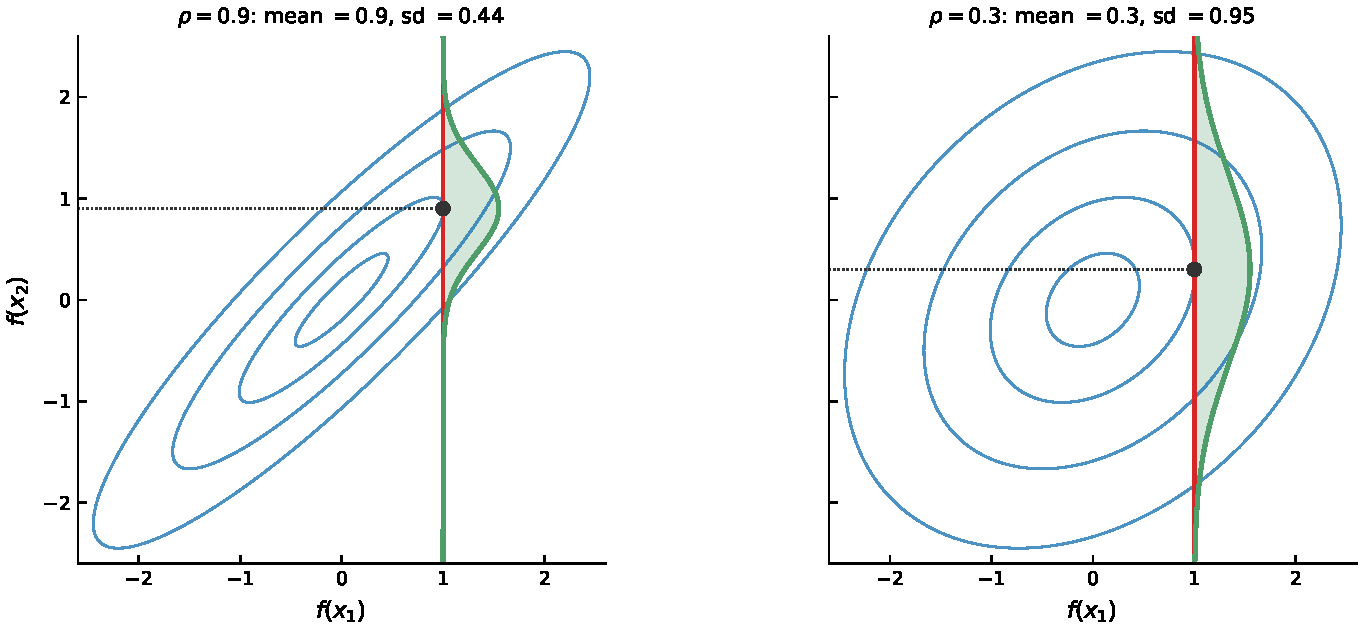
\includegraphics[width=0.95\textwidth]{figs/rep-conditioning}
\end{figure}
\column{0.45\textwidth}
\[
f(x_1) = Z_1, \qquad f(x_2) = \rho Z_1 + \sqrt{1 - \rho^2}\, Z_2
\]
\[
f(x_2) \mid f(x_1) = y \;\sim\; \mathcal{N}\bigl(\rho y,\ 1 - \rho^2\bigr)
\]
\medskip
\chip{$\rho = 0.9$}{mean $0.9y$, standard deviation $0.44$}\\[4pt]
\chip{$\rho = 0.3$}{mean $0.3y$, standard deviation $0.95$}
\end{columns}
\note{
Consider centered function values at two locations.
Let $Z_1$ and $Z_2$ be independent standard Gaussian variables, and set $f(x_1)=Z_1$ and $f(x_2)=\rho Z_1+\sqrt{1-\rho^2}Z_2$.
The values have mean zero, variance one, and covariance $\rho$.

A noiseless observation $f(x_1)=y$ fixes $Z_1=y$.
The conditional value at $x_2$ has mean $\rho y$ and standard deviation $\sqrt{1-\rho^2}$.
This deviation is $0.44$ at $\rho=0.9$ and $0.95$ at $\rho=0.3$.
Stronger correlation gives less remaining uncertainty.
A Gaussian process specifies such joint Gaussian distributions at every finite collection of locations.
}
\end{frame}

\begin{frame}{Prior draws from three kernels}
\begin{center}
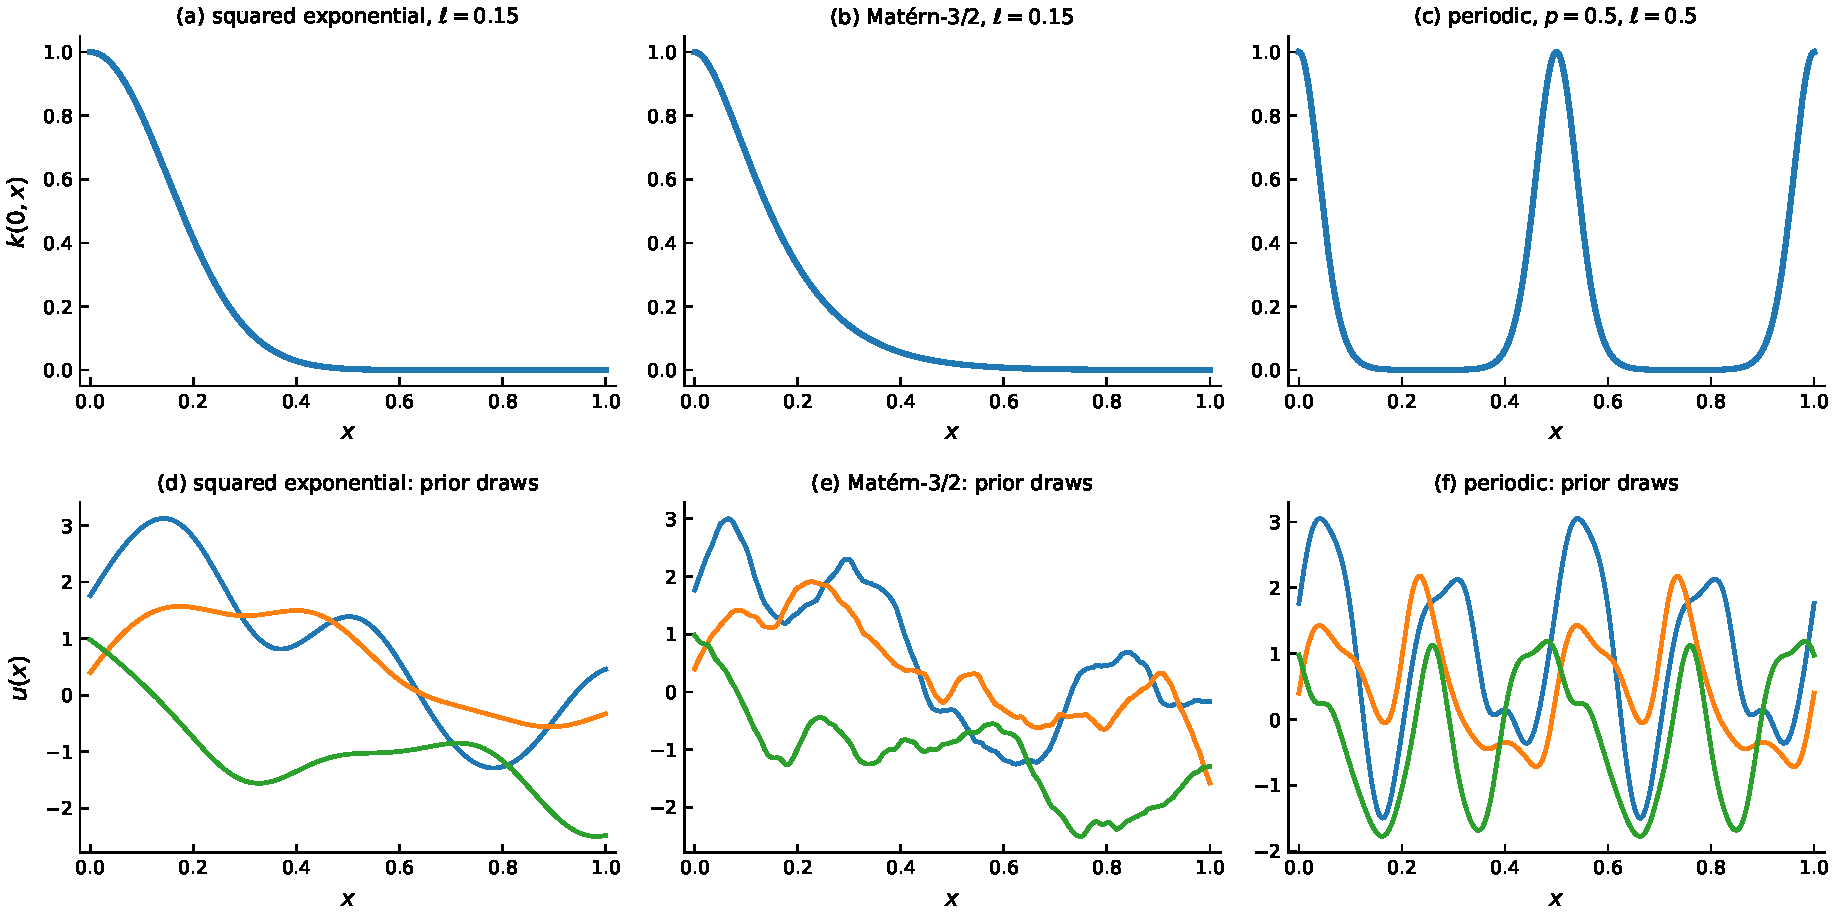
\includegraphics[width=0.66\textwidth]{figs/kernel-gallery}
\end{center}
\centering
\chip{mean absolute slope of the draws}{$5.2$, $8.9$, and $20$}\quad\chip{Gaussian-process model}{the prior specifies a mean and a covariance kernel}
\note{
A Gaussian-process prior specifies a mean function and a covariance kernel.
The displayed draws use zero mean and different kernels.
Squared-exponential draws are smooth, Mat\'ern-$3/2$ draws have rougher slopes, and periodic draws repeat.

At the plotted parameters, the mean absolute slopes over five hundred draws are $5.2$, $8.9$, and $20$.
These values describe these particular prior settings.
Conditioning the prior on measurements gives a posterior distribution.
Its mean is a weighted sum of kernel copies, but it is not a typical random draw.
A posterior mean and a prior sample have different mathematical roles.
}
\end{frame}

\begin{frame}{Gaussian-process reconstruction of the fin profile}
\begin{columns}
\column{0.7\textwidth}
\begin{tikzpicture}
\begin{axis}[rep, height=6.2cm, xmin=0, xmax=1, ymin=-0.6, ymax=1.6, xlabel=$x$, ylabel=$T(x)$, legend pos=north east]
\addplot[only marks, mark=*, mark size=2.4pt, sred] table[x=x, y=y]{data/fin_readings.dat};
\addplot[ink, dashed, line width=1.2pt] table[x=x, y=T]{data/fin_true.dat};
\addlegendentry{true profile}
\steponly{1}{2}{\addplot[sblue, line width=1.6pt] table[x=x, y=mu]{data/gp15.dat};
           \addlegendentry{mean, $\ell = 0.15$}
           \addplot[name path=lo, draw=none] table[x=x, y=lo]{data/gp15.dat};
           \addplot[name path=hi, draw=none] table[x=x, y=hi]{data/gp15.dat};
           \addplot[sblue!25] fill between[of=lo and hi];}
\steponly{2}{2}{\addplot[sgreen, line width=1.6pt] table[x=x, y=mu]{data/gp31.dat};
         \addlegendentry{mean, $\ell = 0.31$, chosen by the readings}
         \addplot[name path=lo3, draw=none] table[x=x, y=lo]{data/gp31.dat};
         \addplot[name path=hi3, draw=none] table[x=x, y=hi]{data/gp31.dat};
         \addplot[sgreen!25] fill between[of=lo3 and hi3];}
\end{axis}
\end{tikzpicture}
\column{0.3\textwidth}
\chip{mean}{$\mathbf{k}(x)^\top(\mathbf{K} + \sigma^2\mathbf{I})^{-1}\mathbf{y}$}\\[4pt]
\chip{variance}{$k(x,x) - \mathbf{k}(x)^\top(\mathbf{K} + \sigma^2\mathbf{I})^{-1}\mathbf{k}(x)$}\\[4pt]
\steponly{1}{2}{\chip{$\ell = 0.15$}{error $10$ percent, half-width in the gap $0.90$}}
\steponly{2}{2}{\chip{$\ell = 0.31$}{error $3.2$ percent, half-width in the gap $0.12$}\\[4pt]
\chip{value at $x = 0.7$}{$0.389$ against the true $0.393$}}
\end{columns}
\note{
Assume a zero-mean Gaussian-process prior and readings $y_i=f(x_i)+\varepsilon_i$ with independent noise of variance $\sigma^2$.
Define $\mathbf{k}_x$ by $(\mathbf{k}_x)_i=k(x,x_i)$.
Conditioning gives mean $m(x)=\mathbf{k}_x^\top(\mathbf{K}+\sigma^2\mathbf{I})^{-1}\mathbf{y}$.
The latent-function variance is $v(x)=k(x,x)-\mathbf{k}_x^\top(\mathbf{K}+\sigma^2\mathbf{I})^{-1}\mathbf{k}_x$.

The mean equals kernel ridge regression with $\lambda=\sigma^2$ for the unnormalized data objective.
The variance excludes the noise of a future measurement.
The band $m(x)\pm2\sqrt{v(x)}$ is pointwise and conditional on the chosen kernel and noise parameters.

With noise standard deviation $0.03$, the largest half-width in the unsensed interval is $0.90$ at $\ell=0.15$ and $1.99$ at $\ell=0.075$.
Shorter correlations leave greater uncertainty between these sensors.
The tested marginal-likelihood maximum selects $\ell=0.31$.
For this synthetic reference, the mean then has relative $L^2$ error $3.2$ percent and maximum gap half-width $0.12$.
These results do not guarantee simultaneous coverage or account for uncertainty in the selected parameters.
}
\end{frame}

\begin{frame}{Choosing the length scale by marginal likelihood}
\begin{columns}
\column{0.6\textwidth}
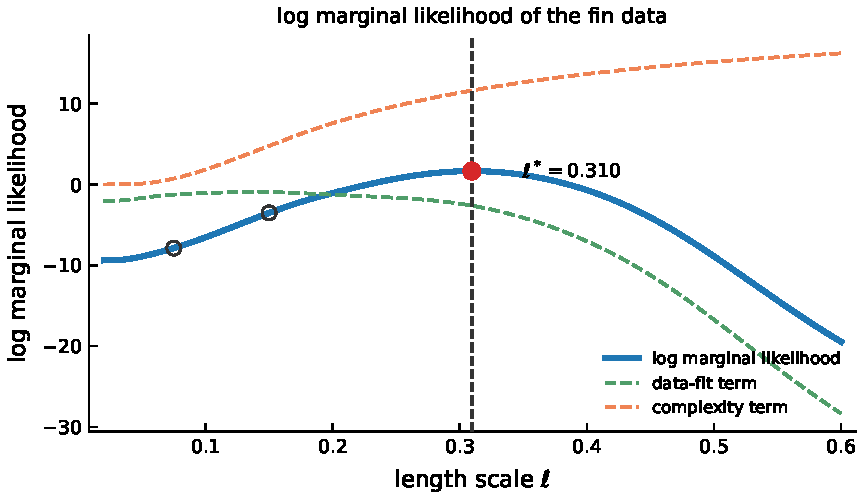
\includegraphics[width=\textwidth]{figs/lml-selection}
\column{0.4\textwidth}
\chip{log marginal likelihood at $\ell = 0.31$}{$1.7$, the maximum}\\[4pt]
\chip{at $\ell = 0.15$ and $0.075$}{$-3.5$ and $-7.9$}\\[4pt]
\chip{length-scale selection}{the posterior band conditions on the selected value}
\end{columns}
\note{
The readings have a joint Gaussian density under the prior-plus-noise model.
The marginal likelihood evaluates that density as a function of the length scale and noise parameters.
Its log contains a quadratic data-fit term and a log-determinant term for the covariance.

For this fin experiment, the log marginal likelihood is $1.7$ at $\ell=0.31$.
It is $-3.5$ at $\ell=0.15$ and $-7.9$ at $\ell=0.075$.
The tested maximum therefore selects $0.31$.
The curve is broad with these few readings, so selecting one length scale does not remove parameter uncertainty.
The plotted posterior bands condition on that selection.
}
\end{frame}

\begin{frame}{Conditioning a kernel prior on $\mathcal{L}u = f$}
\begin{columns}
\column{0.62\textwidth}
\begin{tikzpicture}
\begin{axis}[rep, height=5.6cm, xmin=0, xmax=1, ymin=-0.2, ymax=1.35, xlabel=$x$, ylabel=$u(x)$, legend pos=north east]
\addplot[ink, dashed, line width=1.6pt] table[x=x, y=u]{data/gp_poisson.dat};
\addlegendentry{exact $u$}
\stepfrom{2}{\addplot[sblue, line width=1.6pt] table[x=x, y=mu]{data/gp_poisson.dat};
          \addlegendentry{posterior mean}}
\addplot[only marks, mark=triangle*, mark size=2.2pt, sorange] table[x=x, y=y]{data/gp_poisson_colloc.dat};
\addlegendentry{$25$ points where $f$ is known}
\end{axis}
\end{tikzpicture}
\column{0.38\textwidth}
\small
\[
\operatorname{cov}(u, f) = \mathcal{L}_{x'} k
\]
\[
\operatorname{cov}(f, f) = \mathcal{L}_x \mathcal{L}_{x'} k
\]
\stepfrom{2}{\chip{relative $L^2$ error of the mean}{$3.2 \times 10^{-7}$}\\[4pt]
\chip{condition number of the observation covariance}{$1.4 \times 10^{12}$}}
\end{columns}
\note{
Now place a squared-exponential prior with $\ell=0.2$ on the string displacement.
Applying the linear operator $\mathcal{L}=-d^2/dx^2$ to the covariance gives joint Gaussian distributions for displacement values and load values.
Condition on the known load at twenty-five points and the zero endpoint values.

A linear solve gives the posterior mean.
For the test displacement, its relative $L^2$ error is $3.2\times10^{-7}$.
The differential constraints are imposed at the selected points, so this result is not an exact global PDE solution.
Its accuracy depends on the kernel, constraint locations, and numerical solve.

The observation covariance has condition number $1.4\times10^{12}$.
This limits numerical stability in the experiment.
Closed-form Gaussian conditioning applies to linear observations and differential operators.
Nonlinear differential constraints require additional approximation or inference.
}
\end{frame}

%========================================================================================
\repsection{Families}{Approximating a family of functions}

\begin{frame}{A moving front gives a family of functions}
\begin{columns}
\column{0.42\textwidth}
\centering
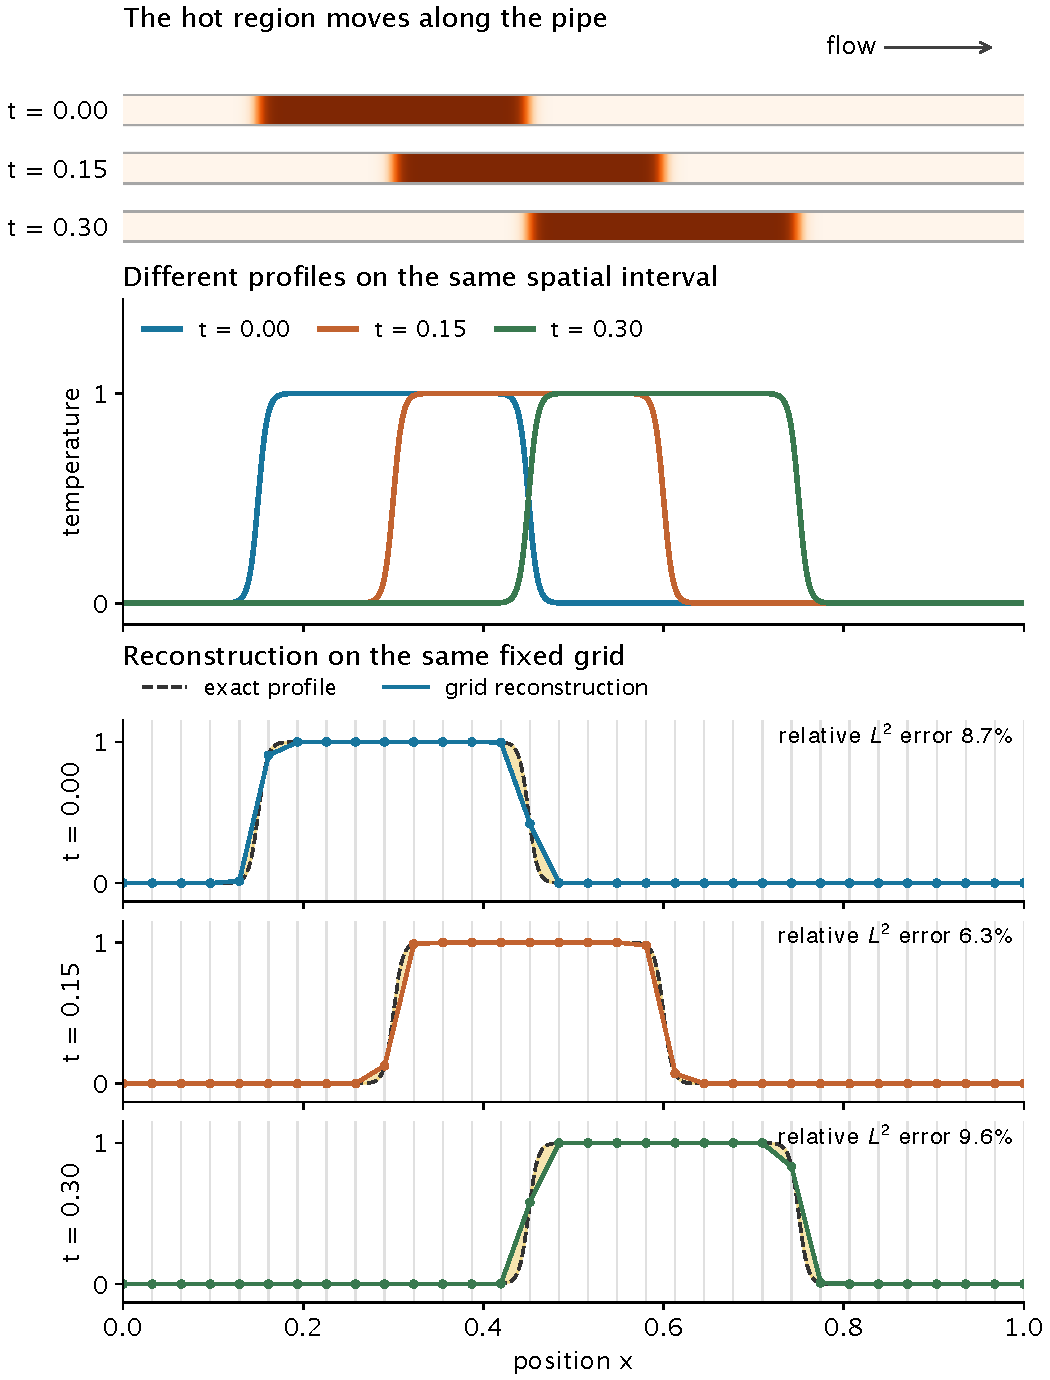
\includegraphics[height=0.8\textheight]{figs/rep-flow-family}
\column{0.58\textwidth}
\small
\[
T(x, t) = T_0(x - ct), \qquad \mathcal{S} = \{T_0(\cdot - ct) \mid 0 \le t \le 0.30\}
\]
\stepfrom{2}{\[
\hat T(x, t) = \sum_i T(x_i, t)\,\phi_i(x)
\]}
\stepfrom{2}{\chip{relative $L^2$ error, $32$ nodes, times $0$, $0.15$, $0.30$}{$8.7$, $6.3$, $9.6$ percent}\\[4pt]
\chip{edge width against node spacing}{$0.01$ against $1/31$}}
\end{columns}
\note{
Consider a hot region transported along a pipe at constant speed $c$ with negligible diffusion.
Its profile translates without changing shape.
At every time, the temperature is a function of position on the same interval.
The representation must approximate this profile at every translated location.

The figure compares the pipe, temperature profiles, and reconstructions on one fixed grid.
The transition width is $w=0.01$, the speed is $c=1$, and the grid has thirty-two nodes with spacing $1/31$.
At times $0$, $0.15$, and $0.30$, the relative $L^2$ reconstruction errors are $8.7$, $6.3$, and $9.6$ percent.
The same grid gives different errors as the edges move between nodes.

The translation rule is $T(x,t)=T_0(x-ct)$.
Knowing $T_0$ and $c$ specifies this family from the single parameter $t$.
A fixed hat basis instead represents every snapshot in the same linear span by changing its coefficients.
A one-parameter family need not lie in a one-dimensional linear space.
Does another fixed basis approximate the entire family more efficiently?
}
\end{frame}

\begin{frame}{The Kolmogorov $n$-width}
\begin{columns}
\column{0.4\textwidth}
\begin{center}
\begin{tikzpicture}[scale=0.85, >={Stealth[length=2.5mm]}, font=\small]
\draw[->, ink] (0,0) -- (2.4,0) node[right] {$(1,0,0)$};
\draw[->, ink] (0,0) -- (0,2.4) node[above] {$(0,1,0)$};
\draw[->, ink] (0,0) -- (-1.5,-1.3) node[below left] {$(0,0,1)$};
\fill[sblue!20, opacity=0.8] (-1.2,0.9) -- (2.2,1.7) -- (1.6,-1.2) -- (-1.8,-2.0) -- cycle;
\node[sblue, font=\scriptsize] at (1.2,1.55) {a plane, two dimensions};
\end{tikzpicture}
\end{center}
\column{0.6\textwidth}
\begin{block}{Kolmogorov $n$-width}
\[
d_n(\mathcal{M}) = \inf_{\dim V = n} \; \sup_{f \in \mathcal{M}} \; \inf_{v \in V} \|f - v\|
\]
\end{block}
\medskip
\chip{three unit spikes, squared distances to any plane}{sum to $3 - 2 = 1$}\quad\chip{worst spike}{at least $\sqrt{1/3} = 0.577$}
\end{columns}
\note{
Consider the unit spikes $\mathbf{e}_1$, $\mathbf{e}_2$, and $\mathbf{e}_3$ in Euclidean $\mathbb{R}^3$.
Project them onto any plane through the origin.
Their squared projection lengths sum to the plane's dimension, two.
Their squared errors therefore sum to one, so at least one error is at least $1/\sqrt3=0.577$.

No plane approximates every spike more accurately than this lower bound.
An exact linear representation needs dimension three, although a position parameter identifies each spike.
A moving localized profile has the same distinction between parameter count and linear-span dimension.

The Kolmogorov $n$-width measures worst-case error in a specified norm.
For each fixed $n$-dimensional subspace, it takes the largest distance over the family.
It then takes the infimum over all such subspaces.
The space is chosen once for the entire family, rather than separately for each profile.
}
\end{frame}

\begin{frame}{Widths of diffusion and transport families}
\begin{columns}
\column{0.7\textwidth}
\begin{figure}
\centering
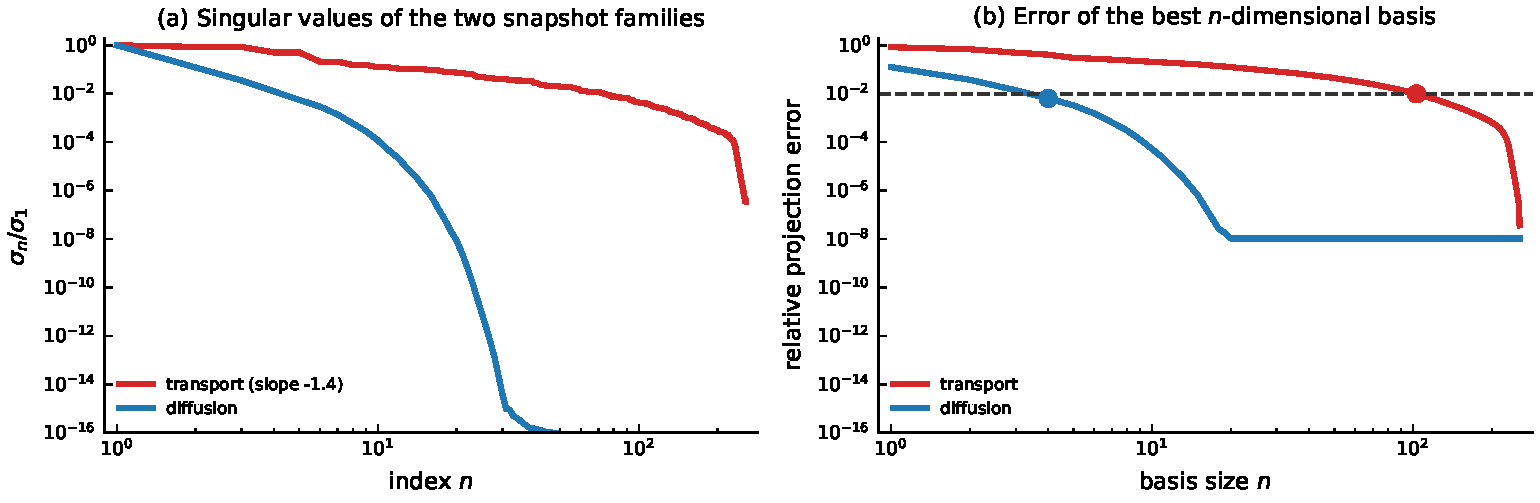
\includegraphics[width=\textwidth]{figs/nwidth}
\end{figure}
\column{0.3\textwidth}
\chip{diffusing pulse, SVD, one percent relative Frobenius error}{four modes}\\[4pt]
\chip{translating pulse, same measure}{$103$ modes}\\[4pt]
\chip{coefficient $k$ under diffusion}{shrinks by $e^{-(2\pi k)^2 t}$}\\[4pt]
\chip{coefficient $k$ under translation}{changes phase only}
\end{columns}
\note{
Translation alone does not force a large width.
Every translate of $\sin(kx)$ belongs to the span of $\sin(kx)$ and $\cos(kx)$.
A narrow pulse with steep edges instead contains many frequencies.
Translation changes their phases without reducing their magnitudes.

For the periodic heat equation with unit diffusivity, each Fourier coefficient decreases by $e^{-(2\pi k)^2t}$.
In the sampled experiments, four modes approximate the diffusion snapshots to one percent relative Frobenius error.
The translating pulse requires $103$ modes for the same metric.

The snapshot SVD minimizes summed squared projection error over the sampled profiles.
The reported relative error is $\|\mathbf{X}-P\mathbf{X}\|_F/\|\mathbf{X}\|_F$.
Kolmogorov width instead concerns the worst member of the full family.
A small snapshot-average error therefore does not establish a small worst-case width.
Can the representation change its locations or selected terms with the profile?
}
\end{frame}

%========================================================================================
\repsection{Adaptive}{Adaptive representations}

\begin{frame}{Particle positions and values under advection}
\begin{columns}
\column{0.62\textwidth}
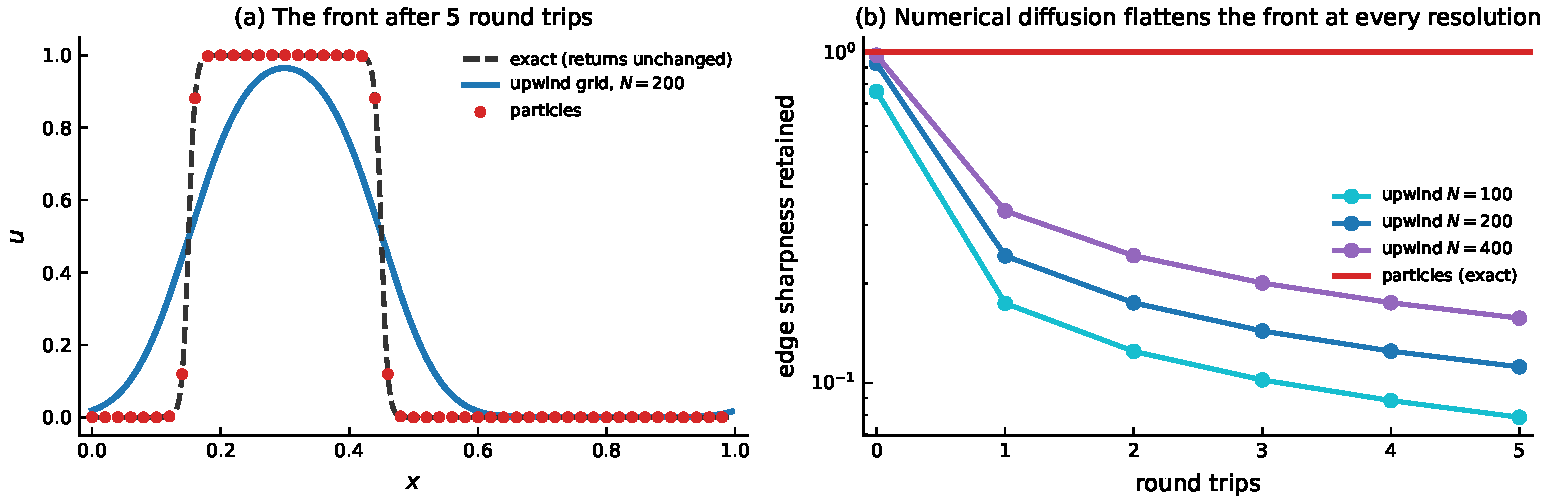
\includegraphics[width=\textwidth]{figs/particles-vs-grid}
\column{0.38\textwidth}
\chip{markers after five round trips}{the front returns unchanged}\\[4pt]
\chip{upwind grid at $100$, $200$, $400$ points}{keeps $8$, $11$, and $16$ percent of the edge steepness}
\end{columns}
\note{
The translated-template formula stores the initial shape and evaluates it at shifted coordinates.
It assumes a known translation law.
Its functions need not belong to one low-dimensional linear space.
Other adaptive representations change their locations, shapes, or selected terms.

A particle representation stores positions and temperature values.
Under pure advection, the values remain constant while the positions follow the flow.
The stored profile returns unchanged after five round trips in this experiment.
Interpolation between particles still introduces reconstruction error.

The first-order upwind comparison uses $T_i^{n+1}=(1-\nu)T_i^n+\nu T_{i-1}^n$ for positive speed and $0<\nu=c\Delta t/h<1$.
Each update averages neighboring values and widens the transition.
The grid retains $8$, $11$, and $16$ percent of the initial edge steepness at $100$, $200$, and $400$ points.
This numerical diffusion comes from the update rule, separately from representation error.
At $\nu=1$, the update shifts grid values without averaging.
}
\end{frame}

\begin{frame}{Gaussian splats with trainable centers and shapes}
\begin{columns}
\column{0.62\textwidth}
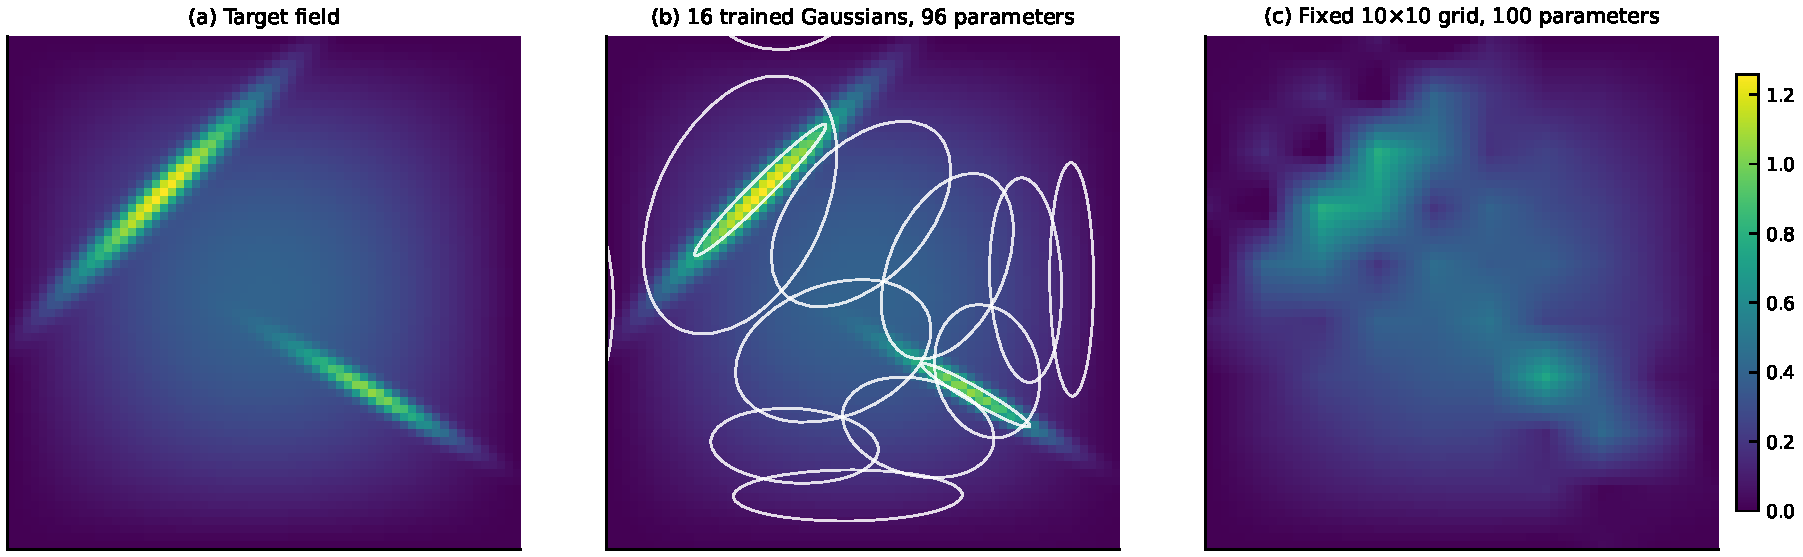
\includegraphics[width=\textwidth]{figs/gaussian-splat}
\column{0.38\textwidth}
\chip{sixteen trained Gaussians, $96$ parameters}{relative $L^2$ error $0.0125$}\\[4pt]
\chip{fixed grid, $100$ coefficients}{relative $L^2$ error $0.30$}
\end{columns}
\note{
A Gaussian element has a center, covariance, and amplitude.
An anisotropic covariance permits a long, narrow shape aligned with a ridge.
Fitting these parameters places the elements near the field's localized variation.
Sixteen trained Gaussians with ninety-six parameters give relative $L^2$ error $0.0125$, compared with $0.30$ for the hundred-coefficient grid.

With centers and covariances fixed, quadratic amplitude fitting gives a linear system.
Training the locations and shapes generally makes the objective non-convex.
This permits adaptation to the target but introduces the possibility of a poor local minimum.
}
\end{frame}

\begin{frame}{Selecting coefficients from a fixed dictionary}
\begin{columns}
\column{0.62\textwidth}
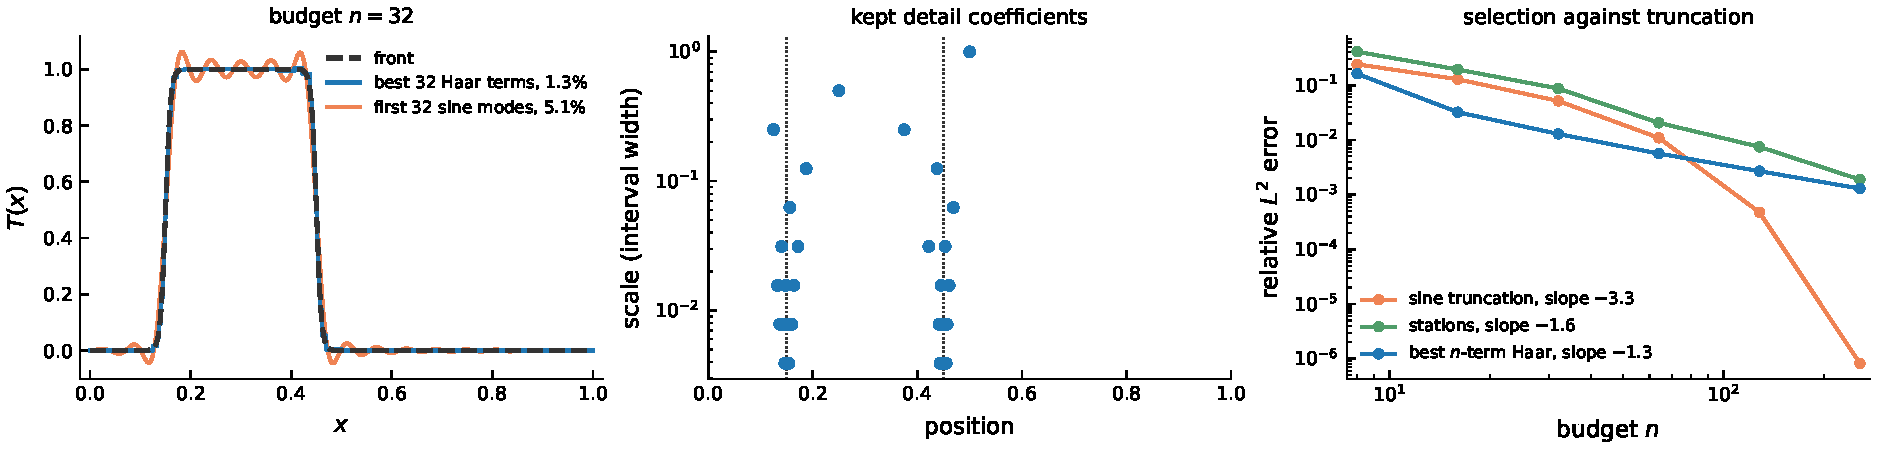
\includegraphics[width=\textwidth]{figs/rep-nterm}
\column{0.38\textwidth}
\chip{relative $L^2$ error, $n=16$, sines, stations, Haar}{$12.8$, $19.3$, $3.2$ percent}\\[4pt]
\chip{relative $L^2$ error, $n=32$, Haar against sines}{$1.3$ against $5.1$ percent}\\[4pt]
\chip{smaller relative $L^2$ error for sines}{near $n = 128$}
\end{columns}
\note{
An orthonormal Haar dictionary permits a different form of adaptation.
Retaining the $n$ largest coefficients minimizes the $L^2$ truncation error among its $n$-term selections.
For the moving front, the selected terms concentrate near the edges.
Their indices change as the edges move.

At $n=16$, the relative $L^2$ errors are $12.8$ percent for sine truncation, $19.3$ percent for station interpolation, and $3.2$ percent for Haar selection.
At $n=32$, Haar selection gives $1.3$ percent compared with $5.1$ percent for sines.
Near $n=128$, the sine truncation resolves the edge width and becomes more accurate in this experiment.

Different profiles select different dictionary subspaces.
The fixed-space restriction in Kolmogorov width therefore does not describe this adaptive approximation.
Storage includes the selected indices as well as the coefficient values.
The underlying resolution and omitted coefficients still limit accuracy.
}
\end{frame}

\begin{frame}{Movable hat nodes on a traveling front}
\begin{columns}
\column{0.7\textwidth}
\begin{tikzpicture}
\begin{axis}[rep, height=6.2cm, xmin=0, xmax=1, ymin=-0.25, ymax=1.25, xlabel=$x$, ylabel=$T(x)$, legend style={at={(0.5,1.02)}, anchor=south, legend columns=2}]
\addplot[only marks, mark=|, mark size=3pt, sblue] table[x=x, y=y]{data/stations32.dat};
\addlegendentry{32 stations}
\steponly{1}{2}{\addplot[muted, dotted, line width=0.9pt, forget plot] table[x=x, y=h1]{data/front_hats0.dat};
         \addplot[muted, dotted, line width=0.9pt, forget plot] table[x=x, y=h4]{data/front_hats0.dat};
         \addplot[muted, dashed, line width=1.1pt, forget plot] table[x=x, y=h2]{data/front_hats0.dat};
         \addplot[muted, dashed, line width=1.1pt, forget plot] table[x=x, y=h3]{data/front_hats0.dat};
         \addplot[ink, dashed, line width=1.2pt, forget plot] table[x=x, y=T]{data/front0.dat};
         \addplot[sblue, line width=1.4pt, forget plot] table[x=x, y=seg]{data/front0.dat};
         \addplot[sorange, line width=1.6pt] table[x=x, y=net]{data/front0.dat};
         \addlegendentry{four movable nodes}
         \foreach \e/\l in {0.15/a, 0.45/b} {
           \edef\tmp{\noexpand\draw[ink, line width=1pt] (axis cs:\e,-0.13) -- (axis cs:\e,-0.03) node[above, font=\noexpand\tiny] {$\l$};
             \noexpand\draw[sorange, <->, >={Stealth[length=1.5mm]}] (axis cs:\e-0.02,-0.08) -- (axis cs:\e,-0.08);
             \noexpand\draw[sorange, <->, >={Stealth[length=1.5mm]}] (axis cs:\e,-0.08) -- (axis cs:\e+0.02,-0.08);}\tmp}
         \node[sorange, font=\tiny] at (axis cs:0.16,-0.16) {$d$};
         \addplot[only marks, mark=triangle*, mark size=3pt, sorange] coordinates {(0.13,-0.2) (0.17,-0.2) (0.43,-0.2) (0.47,-0.2)};}
\steponly{2}{2}{\addplot[muted, dotted, line width=0.9pt, forget plot] table[x=x, y=h1]{data/front_hats30.dat};
         \addplot[muted, dotted, line width=0.9pt, forget plot] table[x=x, y=h4]{data/front_hats30.dat};
         \addplot[muted, dashed, line width=1.1pt, forget plot] table[x=x, y=h2]{data/front_hats30.dat};
         \addplot[muted, dashed, line width=1.1pt, forget plot] table[x=x, y=h3]{data/front_hats30.dat};
         \addplot[ink, dashed, line width=1.2pt, forget plot] table[x=x, y=T]{data/front30.dat};
         \addplot[sblue, line width=1.4pt, forget plot] table[x=x, y=seg]{data/front30.dat};
         \addplot[sorange, line width=1.6pt] table[x=x, y=net]{data/front30.dat};
         \addlegendentry{four nodes, moved with the front}
         \foreach \e/\l in {0.45/a, 0.75/b} {
           \edef\tmp{\noexpand\draw[ink, line width=1pt] (axis cs:\e,-0.13) -- (axis cs:\e,-0.03) node[above, font=\noexpand\tiny] {$\l$};
             \noexpand\draw[sorange, <->, >={Stealth[length=1.5mm]}] (axis cs:\e-0.02,-0.08) -- (axis cs:\e,-0.08);
             \noexpand\draw[sorange, <->, >={Stealth[length=1.5mm]}] (axis cs:\e,-0.08) -- (axis cs:\e+0.02,-0.08);}\tmp}
         \node[sorange, font=\tiny] at (axis cs:0.46,-0.16) {$d$};
         \addplot[only marks, mark=triangle*, mark size=3pt, sorange] coordinates {(0.43,-0.2) (0.47,-0.2) (0.73,-0.2) (0.77,-0.2)};}
\end{axis}
\end{tikzpicture}
\column{0.3\textwidth}
\chip{nodes}{$a - d$, $a + d$, $b - d$, $b + d$, with $d = 0.02$}\\[4pt]
\steponly{1}{2}{\chip{32 stations}{$8.7$ percent}\\[4pt]\chip{four nodes}{$4.9$ percent}}
\steponly{2}{2}{\chip{32 stations, front shifted by $0.3$}{$9.6$ percent}\\[4pt]\chip{four nodes, moved with the front}{$4.9$ percent}}
\vfill
\live{let-the-nodes-move}
\end{columns}
\note{
Place hat nodes near the front edges at $a-d$, $a+d$, $b-d$, and $b+d$.
Here $a$ and $b$ are the edge locations and $d=0.02$.
The nodal values are $0$, $1$, $1$, and $0$.
The piecewise-linear sum rises across the first edge, stays at one, and falls across the second.

The relative $L^2$ error is $4.9$ percent, compared with $8.7$ percent for thirty-two fixed stations.
Increasing $d$ to $0.06$ gives error $19.8$ percent.
The placement and ramp width both affect the fit.

After translation, the fixed-station error becomes $9.6$ percent.
Moving the nodes with the edges retains $4.9$ percent.
A general movable-node representation stores positions as well as coefficients.
Here the known front shape fixes the nodal values, and the translation rule supplies the position changes.
Four movable nodes are therefore not an unrestricted four-number description of an arbitrary function.
}
\end{frame}

\begin{frame}{Fixed nodes and moving nodes}
\begin{center}
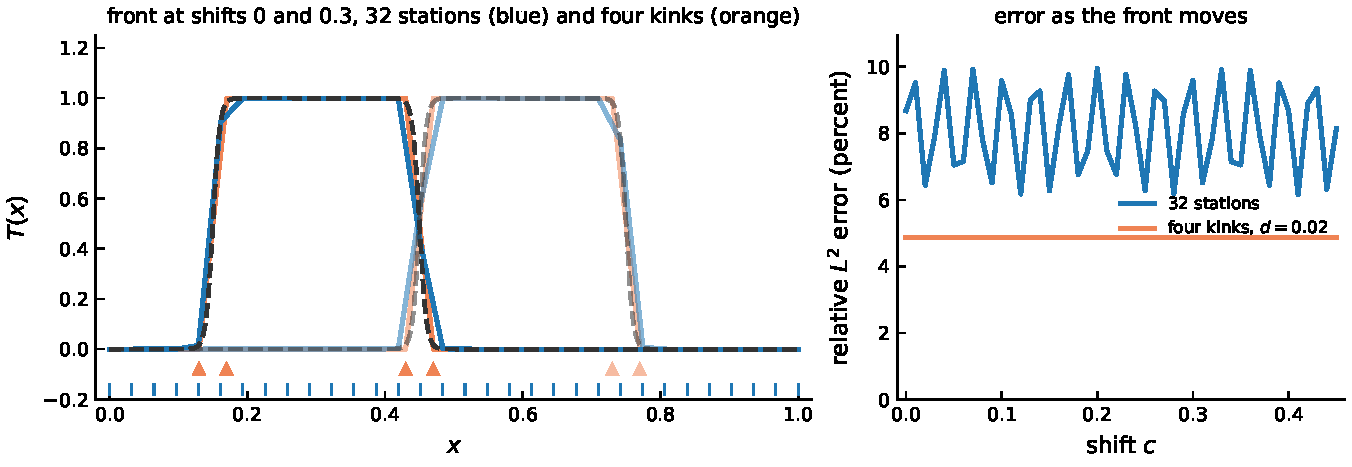
\includegraphics[width=0.62\textwidth]{figs/rep-front-kinks}
\end{center}
\centering
\chip{fixed nodes}{a linear solve, with the projection theorem's guarantee}\quad
\chip{moving nodes}{a generally non-convex fit, without the projection guarantee}
\note{
Fixed hat nodes define a finite-dimensional linear space.
Projection in a specified function inner product gives its unique closest function.
The coefficients follow from a linear system when the hats are independent.

Training the node positions generally makes the fitting objective non-convex.
The representation can then place its resolution near localized features.
The projection theorem no longer guarantees a unique global minimizer.
The approximation benefit and optimization difficulty must both be assessed.
}
\end{frame}

%========================================================================================
\repsection{The fin}{Choosing a representation for the cooling fin}

\begin{frame}{Choosing a representation for the cooling fin}
\begin{columns}
\column{0.5\textwidth}
\begin{figure}
\centering
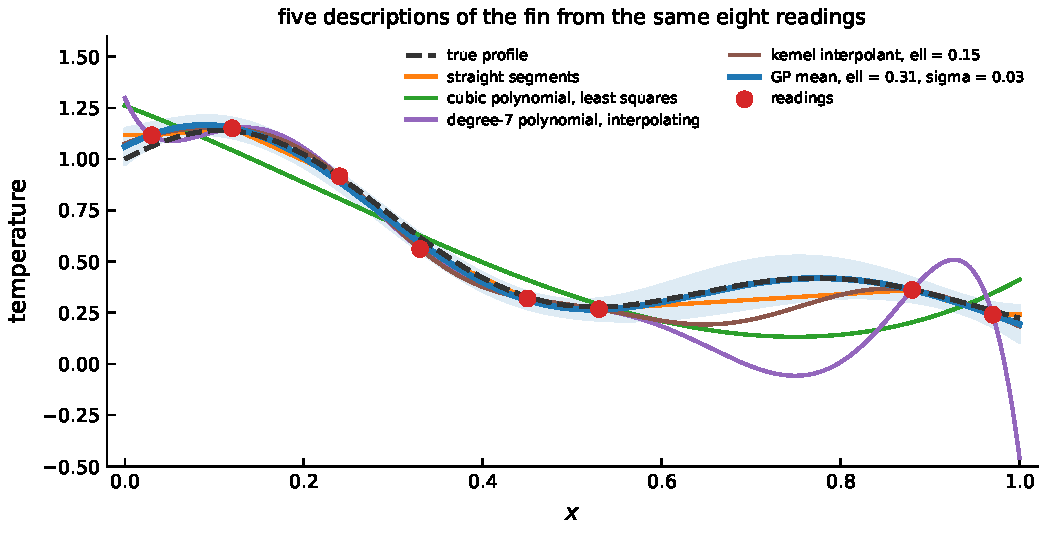
\includegraphics[width=\textwidth]{figs/rep-fin-choice}
\end{figure}
\column{0.5\textwidth}
\scriptsize
\begin{tabular}{@{}lrr@{}}
\toprule
description & relative $L^2$ (\%) & LOO RMSE, fixed $\ell$ \\
\midrule
straight segments & $6.5$ & $0.095$ \\
cubic, least squares & $23$ & $0.310$ \\
degree-7 interpolation & $31$ & $3.57$ \\
kernel interpolant, $\ell = 0.15$ & $11$ & $0.112$ \\
Gaussian-process mean, $\ell = 0.31$ & $3.2$ & $0.034$ \\
\midrule
noise standard deviation & & $0.03$ \\
\bottomrule
\end{tabular}
\end{columns}
\note{
The fin comparison uses the same noisy readings for every method.
Because the experiment is synthetic, its reference profile permits a relative $L^2$ error calculation.
In practice, held-out prediction provides a check when that reference is unavailable.

The leave-one-out calculation omits each reading, fits the rest, and predicts the omitted value.
Its RMSE is measured against the omitted readings.
The noise standard deviation $0.03$ provides a scale for interpreting this error.

The length scales remain fixed at values selected from the full dataset.
These scores therefore diagnose fixed-hyperparameter fits.
Evaluating the full selection procedure requires selecting the parameters again within each training fold.
The Gaussian-process fit performs best in this experiment, without establishing that it is best for every fin.
}
\end{frame}

\begin{frame}{Stored numbers, shape placement, and assumption for each family}
\tiny
\renewcommand{\arraystretch}{1.15}
\begin{tabular}{@{}p{2.6cm}p{3.5cm}p{2.3cm}p{4.2cm}p{2.4cm}@{}}
\toprule
family & stores & shapes placed by & assumes & typical use \\
\midrule
stations, grid & values at fixed points & analyst & linear variation between stations & smooth fields, fixed geometry \\
mesh hats & nodal values & analyst and mesher & piecewise-linear variation & complex geometry \\
sine modes & global coefficients & analyst & smooth odd periodic continuation & smooth pinned fields \\
B-splines, NURBS & coefficients at fixed knots & analyst and CAD & smoothness across knots & engineered shapes \\
wavelets & selected coefficients and indices & analyst, data selects & few active scales per location & localized features \\
POD modes & coefficients on data-derived modes & the snapshot data & a family near a low-dimensional subspace & near-linear families \\
sparse dictionary & few atoms and their indices & the optimizer & few active atoms & few active features \\
particles, SPH, MPM & positions and field values & the dynamics & material motion determines positions & advection, large deformation \\
Gaussian splats & centers, covariances, amplitudes & the optimizer & smooth field with concentrated features & concentrated features \\
level sets & values of an implicit function & analyst and physics & interface as a zero set & moving interfaces \\
kernels, GP & weights, sites, kernel parameters & analyst and data & regularity set by the kernel & scattered data \\
neural fields & network weights & the optimizer & the network's smoothness bias & later chapters \\
latent decoders & codes and a decoder & the optimizer & a low-dimensional nonlinear manifold & later chapters \\
\bottomrule
\end{tabular}
\note{
The table separates stored numbers, shape placement, and assumptions.
A uniform grid supplies its locations by a rule.
Particles require current positions, selected wavelets require indices, and POD coordinates require stored modes.
These reconstruction requirements must be included when comparing storage.

Each representation also has limits.
Sampling permits aliases, sine truncation oscillates near jumps, and an unsuitable kernel length scale distorts the reconstruction.
Training adaptive shapes can stop at a poor local minimum.
The string tests approximation of known functions, while the fin tests reconstruction from incomplete, noisy observations.
}
\end{frame}

%========================================================================================
\repsection{Fields}{From functions to fields}

\begin{frame}{A membrane under a load, $-\Delta u = f$}
\begin{columns}[T]
\column{0.5\textwidth}
\centering
\begin{tikzpicture}
\begin{axis}[width=5.4cm, height=5.4cm, axis equal image, view={0}{90}, colormap/viridis, xmin=0, xmax=1, ymin=0, ymax=1, tick label style={font=\tiny}, label style={font=\tiny}, xlabel=$x$, ylabel=$y$, title={\scriptsize the load $f(x, y)$}, colorbar, colorbar style={width=0.18cm, tick label style={font=\tiny}}]
\stepfrom{2}{\addplot3[surf, shader=interp, mesh/rows=41] table[x=x, y=y, z=z]{data/membrane_f.dat};}
\end{axis}
\end{tikzpicture}
\column{0.5\textwidth}
\centering
\begin{tikzpicture}
\begin{axis}[width=5.4cm, height=5.4cm, axis equal image, view={0}{90}, colormap/viridis, xmin=0, xmax=1, ymin=0, ymax=1, tick label style={font=\tiny}, label style={font=\tiny}, xlabel=$x$, ylabel=$y$, title={\scriptsize the displacement $u(x, y)$, pinned on the edge}, colorbar, colorbar style={width=0.18cm, tick label style={font=\tiny}}]
\stepfrom{3}{\addplot3[surf, shader=interp, mesh/rows=41] table[x=x, y=y, z=z]{data/membrane_u.dat};}
\end{axis}
\end{tikzpicture}
\end{columns}
\small
\[
-\Delta u = -\Bigl(\frac{\partial^2 u}{\partial x^2} + \frac{\partial^2 u}{\partial y^2}\Bigr) = f \text{ on the unit square}, \qquad u = 0 \text{ on its edge}
\]
\stepfrom{3}{\[
u = 0.8\sin(\pi x)\sin(\pi y) + 0.4\sin(2\pi x)\sin(\pi y) + 0.2\sin(\pi x)\sin(3\pi y)
\]}
\note{
A scalar field assigns a value to each point of a spatial domain.
A vector field assigns a vector, such as displacement in a solid.
The string example extends to a membrane on the unit square with zero boundary displacement.
Its load and displacement satisfy $-\Delta u=f$.

The test field is $u=0.8\sin(\pi x)\sin(\pi y)+0.4\sin(2\pi x)\sin(\pi y)+0.2\sin(\pi x)\sin(3\pi y)$.
Applying $-\Delta$ multiplies mode $(j,k)$ by $(j^2+k^2)\pi^2$.
The measured displacement peak is $0.900$ and the load peak is $34.61$.
As on the string, a numerical field representation needs stored numbers and an evaluation rule.
}
\end{frame}

\begin{frame}{Readings on a grid and bilinear reconstruction}
\begin{columns}[T]
\column{0.5\textwidth}
\centering
\begin{tikzpicture}
\begin{axis}[width=5.4cm, height=5.4cm, axis equal image, view={0}{90}, colormap/viridis, xmin=0, xmax=1, ymin=0, ymax=1, tick label style={font=\tiny}, label style={font=\tiny}, xlabel=$x$, ylabel=$y$, title={\scriptsize the field $u$ and the $5 \times 5$ stations}, point meta min=-0.1, point meta max=0.9]
\addplot3[surf, shader=interp, mesh/rows=41] table[x=x, y=y, z=z]{data/membrane_u.dat};
\addplot3[only marks, mark=*, mark size=1.3pt, sred] table[x=x, y=y, z expr=1]{data/membrane_nodes5.dat};
\end{axis}
\end{tikzpicture}
\column{0.5\textwidth}
\centering
\begin{tikzpicture}
\begin{axis}[width=5.4cm, height=5.4cm, axis equal image, view={0}{90}, colormap/viridis, xmin=0, xmax=1, ymin=0, ymax=1, tick label style={font=\tiny}, label style={font=\tiny}, xlabel=$x$, ylabel=$y$, title={\scriptsize bilinear reconstruction from $25$ readings}, point meta min=-0.1, point meta max=0.9]
\stepfrom{2}{\addplot3[surf, shader=interp, mesh/rows=41] table[x=x, y=y, z=z]{data/membrane_bilinear5.dat};}
\end{axis}
\end{tikzpicture}
\end{columns}
\centering
\stepfrom{2}{\chip{$5 \times 5$, $25$ values}{largest gap $22.2$ percent}\quad}
\stepfrom{3}{\chip{$9 \times 9$, $81$ values}{$7.1$ percent}\quad
\chip{$17 \times 17$, $289$ values}{$1.9$ percent}}
\note{
Record the membrane displacement at a grid of five nodes in each direction.
Inside each cell, bilinear interpolation combines its four corner readings.
The reconstructed surface is linear along every coordinate-parallel line within a cell.
The relative sup error from these twenty-five readings is $22.2$ percent.

Nine nodes per direction give eighty-one values and error $7.1$ percent.
Seventeen per direction give $289$ values and error $1.9$ percent.
The smooth-field interpolation error approaches second-order convergence as the spacing decreases.

The value count grows with dimension.
Seventeen nodes per direction require $17$ values on a line, $289$ on a plate, and $4{,}913$ in a solid.
For a tensor grid with $m$ nodes per direction in dimension $d$, storage is $m^d$.
Maintaining spatial resolution therefore requires many more values in higher dimensions.
}
\end{frame}

\begin{frame}{Sine modes and hats in two dimensions}
\begin{columns}[T]
\column{0.24\textwidth}
\centering
\begin{tikzpicture}
\begin{axis}[width=3.6cm, height=3.6cm, axis equal image, view={0}{90}, colormap/viridis, xmin=0, xmax=1, ymin=0, ymax=1, tick label style={font=\tiny}, label style={font=\tiny}, xlabel=$x$, ylabel=$y$, title={\tiny $\sin(\pi x)\sin(\pi y)$}, xtick=\empty, ytick=\empty, xlabel={}, ylabel={}]
\addplot3[surf, shader=interp, mesh/rows=41] table[x=x, y=y, z=z]{data/mode2d_11.dat};
\end{axis}
\end{tikzpicture}
\column{0.24\textwidth}
\centering
\begin{tikzpicture}
\begin{axis}[width=3.6cm, height=3.6cm, axis equal image, view={0}{90}, colormap/viridis, xmin=0, xmax=1, ymin=0, ymax=1, tick label style={font=\tiny}, label style={font=\tiny}, xlabel=$x$, ylabel=$y$, title={\tiny $\sin(2\pi x)\sin(\pi y)$}, xtick=\empty, ytick=\empty, xlabel={}, ylabel={}]
\addplot3[surf, shader=interp, mesh/rows=41] table[x=x, y=y, z=z]{data/mode2d_21.dat};
\end{axis}
\end{tikzpicture}
\column{0.24\textwidth}
\centering
\begin{tikzpicture}
\begin{axis}[width=3.6cm, height=3.6cm, axis equal image, view={0}{90}, colormap/viridis, xmin=0, xmax=1, ymin=0, ymax=1, tick label style={font=\tiny}, label style={font=\tiny}, xlabel=$x$, ylabel=$y$, title={\tiny $\sin(\pi x)\sin(3\pi y)$}, xtick=\empty, ytick=\empty, xlabel={}, ylabel={}]
\addplot3[surf, shader=interp, mesh/rows=41] table[x=x, y=y, z=z]{data/mode2d_13.dat};
\end{axis}
\end{tikzpicture}
\column{0.28\textwidth}
\centering
\begin{tikzpicture}
\begin{axis}[width=4.2cm, height=3.9cm, view={35}{35}, colormap/viridis, xmin=0.2, xmax=0.8, ymin=0.2, ymax=0.8, zmin=0, zmax=1, tick label style={font=\tiny}, title={\tiny a hat on a triangle mesh}, xtick=\empty, ytick=\empty, ztick={0,1}]
\stepfrom{2}{\addplot3[surf, mesh/rows=41, faceted color=black!30] table[x=x, y=y, z=z]{data/hat2d.dat};}
\end{axis}
\end{tikzpicture}
\end{columns}
\small
\[
u(x, y) = \sum_{j, k} a_{jk}\,\sin(j\pi x)\sin(k\pi y), \qquad u_h(x, y) = \sum_i u(\mathbf{x}_i)\,\phi_i(x, y)
\]
\centering
\chip{the membrane's weights}{$a_{11} = 0.8$, $a_{21} = 0.4$, $a_{13} = 0.2$}\quad
\stepfrom{2}{\chip{a hat $\phi_i$}{one at its node, zero at the others, linear on each triangle}}
\note{
On the square, sine modes become products $\sin(j\pi x)\sin(k\pi y)$.
The test membrane uses three such products with coefficients $0.8$, $0.4$, and $0.2$.
These modes are orthogonal and vanish along the boundary.
Their coefficients follow from the corresponding $L^2$ inner products.

On a triangle mesh, a hat equals one at its node and zero at all other nodes.
It is linear on each adjacent triangle.
Weighting the hats by known nodal readings gives a piecewise-planar interpolant.
Boundary-fitted triangular meshes also accommodate irregular domains.

Galerkin's method instead determines the coefficients from $\int\nabla u_h\cdot\nabla\phi_i\,dx=\int f\phi_i\,dx$.
This is the same weak-form construction used for the string.
In two dimensions, it does not generally reproduce the exact solution's nodal values.
Interpolation from known readings and solving for unknown coefficients remain different tasks.
}
\end{frame}

\begin{frame}{What changes in two and three dimensions}
\begin{center}
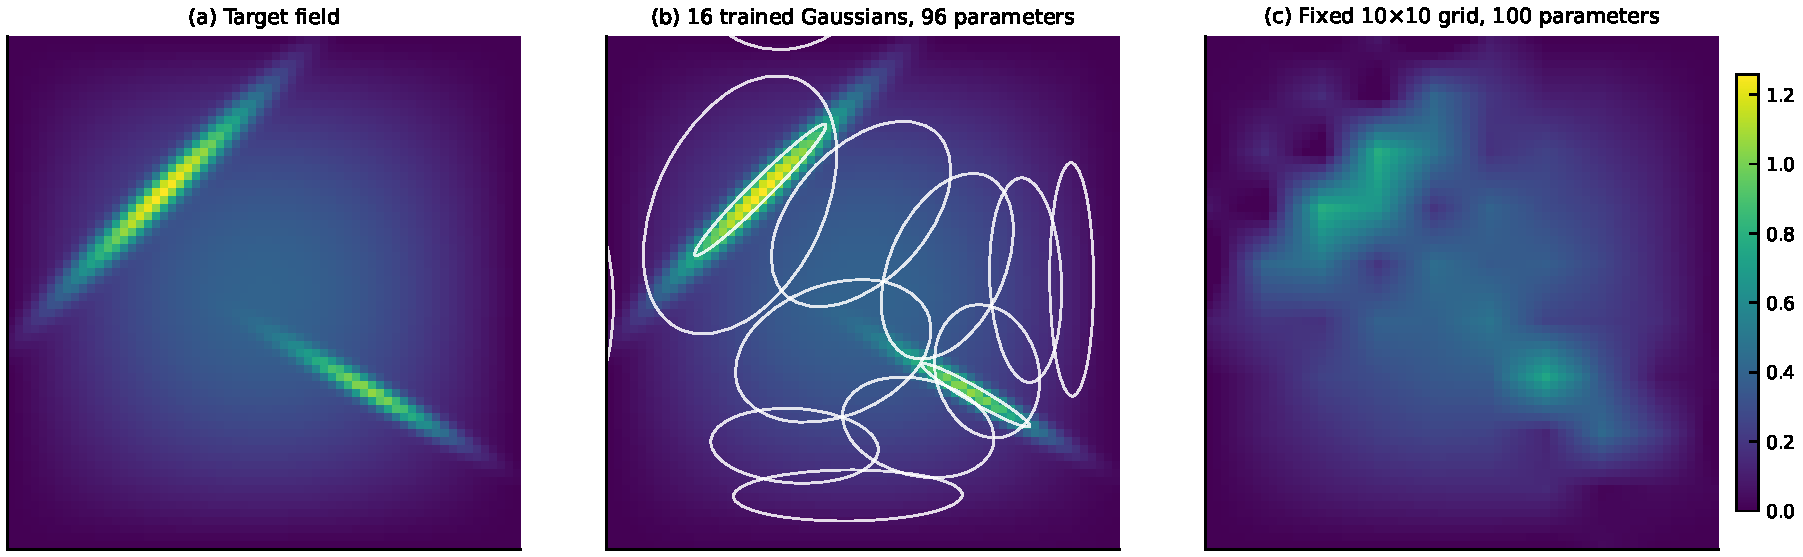
\includegraphics[width=0.72\textwidth]{figs/gaussian-splat}
\end{center}
\centering
\chip{$17$ stations per direction}{$17$ on a line, $289$ on a plate, $4{,}913$ in a solid}\quad
\stepfrom{2}{\chip{a kernel needs only a distance}{$e^{-|\mathbf{x} - \mathbf{x}'|^2/2\ell^2}$, unchanged}}\\[4pt]
\stepfrom{3}{\chip{$H^1$ in two or more dimensions}{finite energy, yet possibly unbounded}\quad
\chip{vector fields}{constraints such as $\nabla \cdot \mathbf{u} = 0$}}
\note{
The Gaussian kernel extends to spatial points through $k(\mathbf{x},\mathbf{x}')=\exp(-|\mathbf{x}-\mathbf{x}'|^2/(2\ell^2))$.
The formula permits scattered sites in any dimension.
It does not remove the need for more measurements to resolve a higher-dimensional field.
The illustrated two-ridge field uses sixteen trained Gaussian elements.

Grid storage grows as a power of dimension.
Seventeen nodes per direction require $17$, $289$, or $4{,}913$ values in one, two, or three dimensions.
Adaptive representations can reduce this count when the field has localized structure.

The function-space assumptions also change.
On an interval, $H^1$ gives a continuous representative.
In higher dimensions, finite energy alone need not define point values.
Sensors that average over a small region instead define bounded measurements on $L^2$.
Vector fields may also require constraints such as $\nabla\cdot\mathbf{u}=0$ for incompressible flow.
}
\end{frame}

\begin{frame}{Summary}
\tableofcontents
\note{
A representation specifies stored numbers and a rule for evaluating a function.
The string examples compare sampled values with coefficients on fixed shapes.
A fixed finite-dimensional family represents its own members without error and approximates a general function outside it.
The error norm determines which features matter.

Projection gives a unique closest function in a closed linear subspace of a Hilbert space.
Density instead asks whether increasing the representation can make the error arbitrarily small.
Neither density nor exact sensor agreement guarantees stable reconstruction from noise.
Kernels specify a function geometry, regularization controls fitting, and Gaussian-process conditioning supplies model-dependent uncertainty.

A family of profiles must be approximated across its full parameter range.
Kolmogorov width measures the limitation of one fixed linear space.
Moving nodes, trained shapes, and selected dictionary terms change the admissible representation with the target.
These choices can reduce approximation error while adding storage or optimization requirements.
In higher dimensions, the same questions apply, but measurement counts and function-space assumptions change.
}
\end{frame}

\end{document}
